%                                     MMMMMMMMM        
%                                                                             
%  MMO    MM   MMMMMM  MMMMMMM   MM    MMMMMMMM   MMD   MM  MMMMMMM MMMMMMM   
%  MMM   MMM   MM        MM     ?MMM              MMM$  MM  MM         MM     
%  MMMM 7MMM   MM        MM     MM8M    MMMMMMM   MMMMD MM  MM         MM     
%  MM MMMMMM   MMMMMM    MM    MM  MM             MM MMDMM  MMMMMM     MM     
%  MM  MM MM   MM        MM    MMMMMM             MM  MMMM  MM         MM     
%  MM     MM   MMMMMM    MM   MM    MM            MM   MMM  MMMMMMM    MM
%
%
%            - META-NET Language Whitepaper | Spanish content -
% 
% ----------------------------------------------------------------------------

\begin{document}

\maketitle

% --------------------------------------------------------------------------
\bsection*{Prólogo --- Preface}

\null
\pagestyle{empty} 

\pagenumbering{Roman} 
\setcounter{page}{3}
\pagestyle{scrheadings}

\vspace*{-4mm}
\begin{Parallel}[c]{78mm}{78mm}
\ParallelLText{\selectlanguage{spanish}
Este documento es parte de una serie de Libros Blancos que promueve el conocimiento sobre las tecnologías del lenguaje y sobre su potencial. Se dirige a educadores, periodistas, políticos y las comunidades lingüísticas, entre otros.

La disponibilidad y el uso de la tecnología lingüística en Europa varían entre los distintos idiomas. En consecuencia, las acciones que se requieren para apoyar la investigación y el desarrollo de las tecnologías de la lengua también son diferentes para cada idioma. Las acciones necesarias dependen de muchos factores, tales como la complejidad de un lenguaje determinado y el tamaño de su comunidad.

META-NET, una red de excelencia financiada por la Comisión Europea, ha llevado a cabo un análisis de los recursos lingüísticos y las tecnologías actuales (p.~\pageref{whitepaperseries}). Este análisis se ha centrado en las 23 lenguas oficiales europeas, así como en otros idiomas importantes, a nivel nacional y regional en Europa. Los resultados de este análisis sugieren que hay muchas lagunas en la investigación relevante para cada idioma. Un análisis más detallado por parte de los expertos y una evaluación de la situación actual contribuirá a maximizar el impacto de las nuevas investigaciones y a minimizar los riesgos.

META-NET se compone de 54 centros de investigación de 33 países que están trabajando con representantes de empresas comerciales, agencias gubernamentales, industria, organizaciones de investigación, empresas de software, proveedores de tecnología y universidades europeas (p.~\pageref{metanetmembers}). Juntos están creando una visión tecnológica común, y al mismo tiempo están desarrollando una agenda estratégica de investigación que, a 10 años vista, permita a las aplicaciones basadas en  tecnología lingüística abordar las deficiencias detectadas.}

\ParallelRText{\selectlanguage{english}
This white paper is part of a series that promotes knowledge about language technology and its potential. It addresses journalists, politicians, language communities, educators and others. 
The availability and use of language technology in Europe varies between languages. Consequently, the actions that are required to further support research and development of language technologies also differ. The required actions depend on many factors, such as the complexity of a given language and the size of its community.

META-NET, a Network of Excellence funded by the European Commission, has conducted an  analysis of current language resources and technologies in this white paper series (p.~\pageref{whitepaperseries}). The analysis focused on the 23 official European languages as well as other important national and regional languages in Europe. The results of this analysis suggest that there are tremendous deficits in technology support and significant research gaps for each language. The given detailed expert analysis and assessment of the current situation will help maximise the impact of additional research.

As of November 2011, META-NET consists of 54 research centres from 33 European countries (p.~\pageref{metanetmembers}). META-NET is working with stakeholders from economy (software companies, technology providers and users), government agencies, research organisations, non-governmental organisations, language communities and European universities. Together with these communities, META-NET is creating a common technology vision and strategic research agenda for multilingual Europe 2020.} 
\ParallelPar
\end{Parallel}

\makefundingnotice

\cleardoublepage

% --------------------------------------------------------------------------
\bsection*{Contenido --- Contents}

\selectlanguage{english}
\renewcommand\contentsname{}
\tableofcontents

\addtocontents{toc}{\protect\thispagestyle{empty}\protect}
\addtocontents{toc}{{\protect\vspace*{-10mm}\protect}}
\addtocontents{toc}{{\Large\textsf{\centerline{LA LENGUA ESPAÑOLA EN LA ERA DIGITAL}}\par}}

\cleardoublepage

% --------------------------------------------------------------------------
\setcounter{page}{1}
\pagenumbering{arabic} 
\pagestyle{scrheadings}

% Start of origin language part
% --------------------------------------------------------------------------
\ssection[Resumen ejecutivo]{Resumen ejecutivo}

\selectlanguage{spanish}

\vspace*{-4mm}
\begin{multicols}{2}
 \selectlanguage{spanish}
  Durante los últimos 60 años, Europa ha adquirido una estructura política y económica singular y, sin embargo, cultural y lingüísticamente todavía es muy diversa. Esto implica que, del portugués al polaco y del italiano al islandés, la comunicación cotidiana entre los ciudadanos europeos, así como la comunicación en el ámbito de los negocios y de la política se enfrenta inevitablemente con las barreras del idioma. Las instituciones de la UE gastan casi mil millones de euros al año en mantener su política de multilingüismo, es decir, traduciendo documentos e interpretando intervenciones orales. Sin embargo, ¿es necesario que estas tareas sigan siendo una carga pesada y costosa? Las modernas tecnologías de la lengua y la investigación lingüística pueden contribuir significativamente a derribar las barreras lingüísticas. En el futuro, las tecnologías lingüísticas, combinadas con dispositivos y aplicaciones inteligentes, serán capaces de ayudar a los europeos a comunicarse fácilmente entre sí y a hacer negocios, incluso si no hablan una lengua común.

\boxtext{La tecnología lingüística construye puentes para el futuro de Europa.}

El mercado único europeo resulta beneficioso para los países que lo integran. Sin embargo, las barreras del idioma pueden suponer un freno para los negocios, especialmente para las pequeñas y medianas empresas, que no tienen los medios económicos para afrontar la situación. La única (e impensable) alternativa a esta Europa multilingüe sería permitir que una sola lengua tomara una posición dominante y terminara reemplazando al resto de lenguas.

El aprendizaje de lenguas extranjeras siempre ha sido una forma habitual de superar las barreras lingüísticas. Sin embargo, sin apoyo tecnológico, llegar a dominar las 23 lenguas oficiales de los Estados miembros de la Unión Europea, sumadas a 60 lenguas más no oficiales, supone un obstáculo insuperable para los ciudadanos de Europa así como para su economía, para el debate político y para el progreso científico.

La solución consiste en invertir en las tecnologías clave para la superación de estas barreras, es decir, las tecnologías lingüísticas. Estas tecnologías ofrecen ventajas enormes, no sólo dentro del mercado común europeo, sino también en las relaciones comerciales con terceros países, especialmente en las economías emergentes. Para lograr este objetivo, y preservar la diversidad cultural y lingüística de Europa, es conveniente considerar las particularidades lingüísticas de todos los idiomas europeos, y analizar el estado actual de las tecnologías lingüísticas para cada uno de ellos. Las tecnologías lingüísticas constituirán en el futuro un puente único entre las lenguas de Europa.

  La traducción automática y las herramientas de procesamiento del habla que están actualmente disponibles en el mercado, aún están lejos de alcanzar este ambicioso objetivo. Los agentes dominantes en estos ámbitos son principalmente empresas de propiedad privada radicadas en América del Norte. Ya en la década de 1970, la UE se dio cuenta de la enorme relevancia de la tecnología lingüística como conductor de la unidad europea, y comenzó a financiar sus primeros grandes proyectos de investigación, como EUROTRA. Al mismo tiempo, se establecieron proyectos nacionales que generaron resultados valiosos, pero que nunca llevaron a una acción europea concertada. En contraste con este esfuerzo financiero altamente selectivo, otras sociedades multilingües, como la India (22 lenguas oficiales) y Sudáfrica (11 lenguas oficiales) han creado recientemente programas nacionales a largo plazo para la investigación lingüística y el desarrollo tecnológico.

\boxtext{Las tecnologías de la lengua, clave para el futuro.}

  Muchas de las aplicaciones de tecnología lingüística utilizan actualmente métodos estadísticos, que se basan en grandes cantidades de datos e ignoran las propiedades intrínsecas de la lengua. Por ejemplo, algunos de los sistemas de traducción más populares traducen automáticamente mediante la comparación de la frase a traducir con centenares de miles de frases previamente traducidas por humanos. La calidad de la producción depende en gran medida de la cantidad y la calidad de la muestra de corpus disponible. Así, mientras que la traducción automática de oraciones sencillas, en idiomas con una cantidad suficiente de texto disponible, puede obtener resultados útiles, los métodos estadísticos puros están condenados al fracaso en el caso de idiomas con cantidades mucho menores de datos, o en el caso de las construcciones sintácticas complejas. Dada esta situación, la Unión Europea ha decidido financiar proyectos tales como EuroMatrix y EuroMatrixPlus (desde 2006) y iTranslate4 (desde 2010) que llevan a cabo investigación básica y aplicada y generan recursos lingüísticos para todos los idiomas europeos. El análisis de las propiedades estructurales más profundas de la lengua es el único camino posible si queremos crear aplicaciones que funcionen bien para toda la gama de las lenguas de Europa.

  La investigación europea en este ámbito ya ha logrado varios éxitos. Por ejemplo, los servicios de traducción de la Unión Europea actualmente están utilizando MOSES, una aplicación de traducción automática de código abierto, que se ha desarrollado principalmente a través de proyectos de investigación europeos. Muchos de los laboratorios de investigación y desarrollo (por ejemplo, IBM y Philips) han cerrado o se han trasladado a otro lugar. En lugar de construir sobre los resultados de sus proyectos de investigación, Europa ha tendido a realizar actividades de investigación aisladas, con menor impacto en el mercado. Incluso el valor económico de estos primeros esfuerzos, puede verse en el número de spin-offs. Una compañía como Trados, que fue fundada en 1984, fue vendida a SDL, con sede en el Reino Unido, en 2005.
  
  \boxtext{Las tecnologías lingüísticas contribuyen a unificar Europa.}
  
  Basándose en los conocimientos acumulados hasta el momento, parece claro que la actual tendencia a la tecnología híbrida, mezcla de procesamiento lingüístico de la lengua con métodos estadísticos, será capaz de reducir la brecha entre todas las lenguas europeas e ir más allá. Como esta serie de “libros blancos” muestra, existen grandes diferencias de preparación entre los diferentes idiomas y estados europeos con respecto a las tecnologías de la lengua. Sin embargo, incluso los idiomas “grandes” como el español, todavía necesitan dedicar más recursos a la investigación con objeto de que las soluciones tecnológicas estén realmente listas para su uso cotidiano. 

  El objetivo a largo plazo de META-NET es introducir tecnología lingüística de alta calidad para todas las lenguas a fin de lograr la unidad política y económica a través de la diversidad cultural. La tecnología ayudará a derribar las barreras existentes y a construir puentes entre las lenguas de Europa. Esto requiere que todas las partes interesadas -- del mundo de la política, de la investigación, la industria y la sociedad --  unan sus esfuerzos de cara al futuro.
  
  Esta serie de “libros blancos” complementa otras acciones estratégicas adoptadas por META-NET (véase el apéndice para un resumen). En el sitio web de META-NET  (http://www.meta-net.eu) puede hallarse información actualizada, como la versión actual del documento de visión META-NET, o la Agenda Estratégica de Investigación (Strategic Research Agenda o SRA).
  
\end{multicols}

\clearpage

% --------------------------------------------------------------------------

\ssection[Un riesgo para nuestras lenguas y un reto para la tecnología lingüística]{Un riesgo para nuestras lenguas y un reto para la tecnología lingüística}

\begin{multicols}{2}
  \selectlanguage{spanish}
  Somos testigos de una revolución digital que está impactando drásticamente en la comunicación y en la sociedad. Esta revolución se ha comparado alguna vez con la invención de la imprenta por Gutenberg. ¿Qué nos puede decir esta analogía sobre el futuro de la sociedad de la información y de nuestras lenguas en particular?

\boxtext{Somos testigos de una revolución digital comparable a la invención de la imprenta por Gutenberg.}

Después de la invención de Gutenberg, los avances reales en la comunicación y el intercambio de conocimientos se lograron mediante esfuerzos tales como la de la Biblia por Lutero a la lengua vernácula. En los siglos siguientes, se desarrollaron técnicas culturales para manejar mejor el procesamiento del lenguaje y el intercambio de conocimiento:

\medskip
\begin{itemize}
  \item la estandarización ortográfica y gramatical de las principales lenguas permitió la rápida difusión de nuevas ideas científicas e intelectuales; 
  \item	el desarrollo de las lenguas oficiales hizo posible que los ciudadanos pudieran comunicarse dentro de ciertos límites (a menudo políticos);
  \item	la enseñanza de lenguas y las traducciones favorecieron los  intercambios entre las distintas lenguas y culturas;
  \item	la creación de editoriales y de directrices bibliográficas aseguraron la calidad y disponibilidad de material impreso;
  \item	la creación de distintos medios de comunicación como periódicos, radio, televisión, libros y otros formatos satisfizo las diferentes necesidades de comunicación. 

\end{itemize}

  En los últimos veinte años, la tecnología de la información ha ayudado a automatizar y facilitar muchos de los procesos:

\begin{itemize}
  \item el software de autoedición ha sustituido la mecanografía y la composición;
  \item Microsoft PowerPoint ha sustituido las transparencias para retroproyector;
  \item el correo electrónico envía y recibe documentos más rápido que una máquina de fax;
  \item Skype ofrece llamadas baratas de telefonía por Internet y organiza reuniones virtuales;
  \item los formatos de audio y de codificación de vídeo facilitan el intercambio de contenido multimedia;
  \item los motores de búsqueda basada en palabras clave proporcionan acceso a las páginas web;
  \item servicios en línea como Google Translate producen traducciones rudimentarias de forma rápida;
  \item las plataformas de medios sociales como Facebook, Twitter y Google+ facilitan la comunicación, la colaboración y el intercambio de información.;

\end{itemize}

  A pesar de que tales herramientas y aplicaciones son útiles, no son todavía capaces de dar soporte a una sociedad europea multilingüe y sostenible, donde la información y las mercancías puedan circular libremente.

\subsection{Las fronteras lingüísticas son un obstáculo para la Sociedad de la Información Europea}
  
  No podemos predecir exactamente como será la sociedad de la información del futuro, pero muy probablemente la gran revolución en la tecnología de la comunicación será relacionar de maneras innovadoras a las personas que hablan diferentes idiomas. Más idiomas y más contenidos interactuarán con nuevos  medios de comunicación en un mismo espacio económico y de información globalizado. La actual popularidad de las redes sociales (Wikipedia, Facebook, Twitter, YouTube, y, recientemente, Google +) es sólo la punta del iceberg.

\boxtext{Un espacio económico y de información globalizado supone una mayor cantidad de lenguas, hablantes y contenido.}

  Hoy en día, podemos transmitir gigabytes de texto alrededor del mundo en pocos segundos, incluso antes de reconocer que el mensaje es en un idioma que no entendemos. Según un reciente informe de la Comisión Europea, el 57\% de los usuarios europeos de Internet adquieren bienes y servicios en un idioma distinto de su lengua materna. (El idioma más común es el inglés, seguido del francés, el alemán y el español.) El 55\% de los usuarios leen contenidos en un idioma extranjero, mientras que sólo el 35\% usa otra lengua para escribir comentarios, correos electrónicos o publicar contenido en la Web \cite{EC1}.  Hace algunos años el inglés era la lengua franca de la Web -la gran mayoría de los contenidos estaba en inglés- pero la situación ha cambiado drásticamente. La cantidad de contenido en línea en otras lenguas europeas (así como asiáticas) se ha disparado.

  Curiosamente, esta brecha digital causada por las barreras lingüísticas no recibe mucha atención en los medios y, sin embargo, la cuestión que se plantea es crucial: ¿Qué idiomas europeos prosperarán en la red y en la sociedad digital, y cuáles están condenados a desaparecer?


\subsection{Nuestras lenguas en peligro}

  Así como la imprenta ayudó a intensificar el intercambio de información en Europa, también llevó a la extinción de muchas lenguas europeas. Ciertas lenguas regionales y minoritarias, como el córnico y el dálmata, tuvieron una producción impresa escasa y su transmisión se limitó a las formas orales, lo que a su vez limitó su ámbito de uso. ¿Tendrá  Internet el mismo impacto en nuestras lenguas?

  Los aproximadamente 80 idiomas de Europa son uno de sus bienes culturales más ricos e importantes, y una parte vital de su singular modelo social \cite{EC2}.
  Si bien algunos de sus idiomas, como el inglés y el español, probablemente sobrevivan en el mercado digital emergente, muchos otros podrían convertirse en irrelevantes en una sociedad en red. Esto debilitaría la posición global de Europa, e iría en contra del objetivo estratégico de garantizar la participación equitativa de todos los ciudadanos europeos, independientemente de su idioma. 
  
  De acuerdo con un informe de la UNESCO en materia de multilingüismo, las lenguas son un medio esencial para el disfrute de derechos fundamentales como la expresión política, la educación y la participación en la sociedad \cite{Unesco1}.  

\subsection{La tecnología lingüística es clave en el desarrollo de muchas aplicaciones}

En el pasado reciente, la mayoría de la inversión destinada a la preservación de las lenguas se centraban en la enseñanza de idiomas y en la traducción. Según una estimación, el mercado europeo de traducción, interpretación, localización de software y globalización de sitios web fue de 8.4 mil millones de euros en 2008 y se espera que crezca en un 10\% anual \cite{EC3}.    Sin embargo, esta cifra sólo cubre una pequeña proporción de las necesidades actuales y futuras de la comunicación entre lenguas. La solución más efectiva para garantizar el multilingüismo en la Europa del futuro pasa por el uso de tecnologías apropiadas, de la misma forma que recurrimos a la tecnología para resolver nuestras necesidades de transporte, de energía y de atención a la discapacidad, entre otras.

La tecnología lingüística (orientada a todas las formas de texto escrito y discurso hablado) ayuda a las personas a colaborar entre ellas, a hacer negocios, a compartir conocimientos y a participar en los debates sociales y políticos, independientemente de las barreras idiomáticas y de las habilidades informáticas. A menudo, opera de forma invisible dentro de sistemas de software complejos para ayudarnos a:

\begin{itemize}
  \item	encontrar información con un motor de búsqueda por Internet;
  \item	comprobar la ortografía y la gramática en un procesador de textos;
  \item	ver recomendaciones de productos en una aplicación de comercio electrónico;
  \item	escuchar las instrucciones verbales de un sistema de navegación para automóviles;
  \item	traducir páginas web a través de un servicio en línea. 
\end{itemize}

Las tecnologías de la lengua consisten en una serie de aplicaciones básicas que operan en un marco de aplicación más amplio. El propósito de la serie de White Papers de META-NET es describir el grado de preparación de cada una de las lenguas europeas en estas tecnologías básicas. 

\boxtext{Europa necesita tecnología lingüística robusta y asequible para todos los idiomas europeos.}

Para mantener nuestra posición en la vanguardia de la innovación global, Europa necesitará disponer de tecnologías lingüísticas adaptadas a todos los idiomas europeos, que sean sólidas, asequibles y estén perfectamente integradas en los entornos de software clave. En un futuro cercano, sin la tecnología lingüística, no seremos capaces de lograr una experiencia de usuario interactiva, multimedia y multilingüe realmente efectiva.

\subsection{Oportunidades para la tecnología lingüística}

En el mundo de la imprenta, el gran avance tecnológico fue la duplicación rápida de la imagen de un texto (una página), utilizando una prensa. Los seres humanos aún tenían que hacer el trabajo laborioso de buscar, leer, traducir y resumir el conocimiento. Tuvimos que esperar hasta Edison para grabar el lenguaje hablado, y en este caso también su tecnología simplemente hacía copias analógicas.

Las tecnologías lingüísticas son capaces de  automatizar los procesos mismos de traducción, producción de contenidos y gestión del conocimiento para todos los idiomas europeos. También pueden servir para construir interfaces intuitivas, basadas en lenguaje humano (escrito o hablado) para electrodomésticos, maquinaria, vehículos, computadoras y robots. Las aplicaciones comerciales e industriales de estas tecnologías se encuentran todavía en las primeras etapas de desarrollo, sin embargo, los éxitos de la I + D están creando una ventana real de oportunidades. Por ejemplo, la traducción automática ya es razonablemente precisa en áreas concretas, y existen aplicaciones experimentales que proporcionan información multilingüe y gestión del conocimiento, así como producción de contenidos, en muchas lenguas europeas.

Como ocurre con la mayoría de las tecnologías, las primeras aplicaciones lingüísticas, como las interfaces basadas en voz y los sistemas de diálogo, se desarrollaron para ámbitos altamente especializados, y con frecuencia su rendimiento es limitado. Sin embargo, existen grandes oportunidades de mercado en ámbitos como la educación o el ocio, con la integración de tecnología lingüística en juegos, en divulgación del patrimonio cultural, en paquetes de entretenimiento educativo, en bibliotecas, entornos de simulación y programas de capacitación. Los servicios de información móvil, el software de aprendizaje de idiomas, los entornos de e-learning, las herramientas de autoevaluación y el software de detección de plagio son sólo algunas de las áreas de aplicación en las que la tecnología lingüística puede desempeñar un papel importante. La popularidad de las redes sociales como Twitter y Facebook sugieren necesidades adicionales para esta tecnología, como por ejemplo, control de foros, resumen de discusiones, tendencias de opinión, detección de respuestas emocionales o identificación de  infracciones de derechos de autor, entre otros.

\boxtext{La tecnología lingüística ayuda a superar la „discapacidad” de la diversidad lingüística.} 

La tecnología lingüística representa una gran oportunidad para la Unión Europea y puede ayudar a abordar el complejo tema del multilingüismo en Europa - el hecho de que distintas lenguas convivan de forma natural en empresas, organizaciones y escuelas europeas. Los ciudadanos tienen que comunicarse a través de estas fronteras lingüísticas que cruzan el Mercado Común Europeo, y la tecnología lingüística puede ayudar a superar esta barrera final, a la vez que apoya el uso libre y abierto de cada una de las lenguas individuales. Mirando aún más hacia adelante, una tecnología lingüística multilingüe e innovadora, proporcionará un punto de referencia a nuestros socios a nivel mundial, cuando empiecen a atender a sus propias comunidades multilingües. La tecnología lingüística puede verse como una forma de tecnología „asistencial” que ayuda a superar la ”discapacidad” de la diversidad lingüística y hace que las comunidades lingüísticas sean más accesibles entre sí.

Por último, un campo activo de investigación es el innovador uso de la tecnología lingüística en operaciones de rescate en zonas de desastre, donde la eficiencia puede ser una cuestión de vida o muerte: los robots inteligentes del futuro, dotados de capacidades multilingües tendrán un potencial aumentado para salvar vidas.

\subsection{Retos de la tecnología lingüística}

Aunque la tecnología lingüística ha hecho progresos considerables en los últimos años, el ritmo actual de progreso tecnológico y la innovación en los productos es demasiado lento. Incluso tecnologías ampliamente utilizadas, como la corrección ortográfica y gramatical de los procesadores de texto, sólo están disponibles para unos cuantos idiomas. 

\boxtext{El ritmo actual de progreso tecnológico y la innovación en los productos es demasiado lento.}

Los servicios de traducción automática en línea, aunque son útiles para generar de forma rápida una aproximación razonable al contenido de un documento, todavía no resultan prácticos cuando la traducción debe ser muy exacta. Debido a la complejidad del lenguaje humano, el desarrollo del software que lo modela y su puesta a prueba en el mundo real resulta un proceso largo y costoso que requiere de financiación continuada. Europa debe pues mantener su papel pionero a la hora de enfrentarse a los desafíos tecnológicos de una comunidad multilingüe inventando  nuevos métodos para acelerar el desarrollo transversal de esta. Estos nuevos  métodos incluyen tanto avances computacionales como técnicas emergentes, como por ejemplo, el crowdsourcing.

\subsection{Adquisición del lenguaje por los seres humanos y por las máquinas}

Para ilustrar cómo manejan el lenguaje los ordenadores y por qué es difícil programarlos para usarlo, vamos a examinar brevemente la manera en que los seres humanos adquieren sus primeras y segundas lenguas, y luego cómo funcionan las tecnologías lingüísticas.

\boxtext{Los seres humanos adquieren capacidades lingüísticas de dos maneras diferentes: aprendiendo de los ejemplos y aprendiendo las reglas gramaticales subyacentes.}

Los seres humanos adquieren capacidades lingüísticas de dos maneras diferentes. Los bebés aprenden un idioma al escuchar las interacciones reales entre sus padres, hermanos y personas del ámbito familiar. Desde los dos años, los niños producen sus primeras palabras y frases cortas. Esto sólo es posible porque los seres humanos tienen una predisposición genética a imitar y racionalizar lo que escuchan.

Aprender un segundo idioma a una edad avanzada requiere más esfuerzo, sobre todo si la persona no se encuentra inmersa en una comunidad lingüística de hablantes nativos. En la escuela, los idiomas extranjeros se adquieren a través del aprendizaje explícito del vocabulario y la gramática, haciendo ejercicios, aplicando reglas abstractas y viendo ejemplos. El aprendizaje de una lengua extranjera se hace más difícil con la edad. 

Existen un paralelismo claro entre estas dos maneras de aprender lenguas en los seres humanos y los dos tipos principales de sistemas de tecnología lingüística: los sistemas estadísticos o basados en los datos, y los sistemas basados en reglas.  

Los sistemas estadísticos obtienen conocimiento lingüístico a partir de grandes colecciones de textos concretos. El algoritmo de aprendizaje automático „aprende” cómo se traducen las palabras, las frases cortas y, por último, las oraciones completas. Los textos no son siempre fáciles de obtener. Si bien para entrenar ciertas aplicaciones, por ejemplo, un corrector ortográfico, es suficiente usar texto en un solo idioma, para entrenar un sistema de traducción automática se precisan  textos paralelos, en dos o más lenguas. El enfoque estadístico puede requerir millones de frases y su rendimiento aumenta con la cantidad de texto analizado. Esta es una de las razones por la que los proveedores de motores de búsqueda están dispuestos a recoger tanto material escrito como sea posible. Servicios como Google Search y Google Translate se basan en métodos estadísticos. La gran ventaja de la estadística es que la máquina aprende rápidamente en una serie sucesiva de ciclos de entrenamiento, a pesar de que la calidad del resultado puede variar de forma aparentemente arbitraria.

La estrategia alternativa es la construcción de sistemas basados en reglas. Expertos lingüistas e informáticos primero tienen que codificar el conocimiento gramatical o las reglas de traducción y compilar diccionarios y listas de vocabulario. Esto requiere una gran inversión en tiempo y esfuerzo. Algunos de los principales sistemas de traducción automática basados en reglas han sido objeto de constante desarrollo durante más de veinte años. La gran ventaja de los sistemas basados en reglas es que los expertos tienen un control directo sobre el procesamiento del lenguaje. Esto hace que sea posible corregir errores sistemáticos y dar información detallada al usuario, especialmente cuando los sistemas de reglas se utilizan para el aprendizaje de idiomas. Sin embargo, debido a su alto coste, este tipo de sistemas sólo han sido desarrollados para los idiomas mayoritarios.

Como las ventajas e inconvenientes de los sistemas estadísticos y de los basados en reglas tienden a ser complementarios, la investigación actual se centra en los enfoques híbridos, que combinan las dos metodologías. Sin embargo, estos métodos de momento han tenido más éxito en los centros de investigación que en las aplicaciones industriales.

Como hemos visto en este capítulo, muchas aplicaciones de las más comunes dependen en gran medida la tecnología lingüística. Por su condición multilingüe, esto es particularmente crítico en el espacio europeo de la información. Aunque la tecnología lingüística ha hecho considerables progresos en los últimos años, todavía hay un enorme potencial para mejorar su calidad. En las siguientes secciones, vamos a describir el papel del español en la sociedad europea de la información y evaluar el estado actual de la tecnología lingüística para el español.

\end{multicols}

\clearpage

% --------------------------------------------------------------------------
\ssection[El español en la Sociedad de la Información Europea]{El español en la Sociedad de la Información Europea}

\begin{multicols}{2}
\selectlanguage{spanish}
\subsection{Datos generales}

El español es hoy uno de los idiomas con más peso demográfico en el mundo. Según Ethnologue \cite{ethnologue} es el segundo idioma más hablado en términos de hablantes nativos después del chino. Alrededor del 6\% de la población mundial, o sea más de 400 millones de hablantes, tienen el español como primera lengua.

El español es la lengua oficial de España, donde se originó como una evolución del latín vulgar, pero la mayoría de los hablantes del español se encuentran en América Latina. De todos los países con mayoría de hablantes de español, sólo España y Guinea Ecuatorial se encuentran fuera de América. México tiene el mayor número de hablantes nativos. A nivel nacional, el español es el idioma oficial de Argentina, Bolivia, Chile, Colombia, Costa Rica, Cuba, República Dominicana, Ecuador, El Salvador, Guatemala, Honduras, México, Nicaragua, Panamá, Paraguay, Perú, Puerto Rico, Uruguay y Venezuela \cite{atlasspanish}.

En América, el español coexiste con una multitud de lenguas indígenas, algunas de ellas también co-oficiales con el español en sus respectivos países, como el quechua y el aymara en Perú y Bolivia, y el guaraní en Paraguay. En general, la situación se puede caracterizar como diglósica, siendo el español el idioma de prestigio social, mientras que el otro idioma se utiliza como vehículo de comunicación en el ámbito familiar. El español funciona efectivamente como una koiné y se caracteriza por su homogeneidad lingüística, especialmente entre los hablantes educados, sin olvidar que cuenta con diversas variedades sociolingüísticas y geolingüísticas.

En España y en algunas partes del mundo de habla española, pero no en todas, el español recibe el nombre de castellano, además de español, es decir, el idioma de la región de Castilla, en contraste con otros idiomas que se hablan en España, y que son co-oficiales en sus territorios, como el catalán, el gallego y el vasco.

A pesar de su homogeneidad en general, existen variaciones, principalmente entre la lengua hablada en las zonas centro y norte de España, y la que se habla en gran parte del sur de España, las Islas Canarias y América Latina. Aparte de las variaciones léxicas locales, es bien conocida la diferente pronunciación de la letra c ante las vocales e y i (como en la palabra Barcelona), siendo una fricativa sorda dental / θ /  en la primera zona y una sibilante / s / en la segunda. Otras variaciones afectan al uso de los pronombres de segunda persona: tú o vos, según las zonas, para el singular, y ustedes o vosotros, para el plural.


\subsection{Particularidades de la Lengua Española}

La fonología española presenta un sistema de cinco vocales. El español es una lengua flexiva, con un sistema de dos géneros y alrededor de cincuenta formas verbales conjugadas, pero flexión limitada de sustantivos, adjetivos y determinantes. Utiliza preposiciones y, por lo general, aunque no siempre, los adjetivos se colocan detrás de los sustantivos, como en la mayoría de las otras lenguas románicas. Su sintaxis es generalmente sujeto-verbo-objeto, aunque las variaciones son frecuentes. \cite{spanishgram}

\boxtext{La homofonía es una fuente de posibles errores que los correctores ortográficos y gramaticales deben ser capaces de detectar y corregir.}

La sintaxis del español marca de forma explícita los objetos directos humanos, que van precedidos por la preposición "`a"':
\begin{itemize}
  \item[] \textit{Vi a María} pero \textit{Vi la película}
\end{itemize}
  
Puede usarse un pronombre de objeto indirecto (le, les) “redundante“  incluso en presencia de una frase nominal de objeto indirecto explícita:

\begin{itemize}
  \item[] \textit{Le di las llaves a María.}
\end{itemize}

En lo que respecta a los pronombres de sujeto, el español, como la mayoría de lenguas románicas, permite que no estén presentes de froma explícita, de manera que el verbo flexionado puede aparecer solo. En comparación con otras lenguas romances, el español tiene una sintaxis un poco más libre, con menos restricciones en el orden de las palabras.

Debido al prolongado contacto con otras lenguas, el léxico español contiene préstamos del vasco/ibero, germánico, árabe y de lenguas indígenas americanas, aunque alrededor de un 94\% de su vocabulario proviene íntegramente del latín.

La ortografía española es mucho más transparente que la ortografía del inglés, por ejemplo. La pronunciación de una palabra puede deducirse fácilmente a partir de su forma escrita. No obstante, algunas de las reglas del sistema de escritura conducen potencialmente a la homofonía. Estas incluyen la <h> muda o (a/ ha), la falta de distinción entre <b> y <v> (baca / vaca), o <g> y <j> antes de <e> o <i> (deje / general), así como algunas fusiones dialectales, como la existente entre <y> y <ll> (pollo / poyo), y entre <c> o <z> y <s> (tensión / atención). Así, la misma pronunciación puede escribirse de diversas maneras. Esta es una fuente de posibles errores que los correctores ortográficos y gramaticales deben ser capaces de detectar y corregir.

El español escrito señala  de manera inequívoca el acento fonético a través de una serie de reglas ortográficas. El acento por defecto está en la penúltima sílaba de las palabras que terminan en vocal, <n> o <s> y en la última sílaba, cuando la palabra termina en cualquier consonante que no sea <n> o <s>. Las palabras que no se acentúan por defecto llevan un acento gráfico (agudo) sobre la vocal acentuada.

En español las mayúsculas se usan relativamente poco, comparado con otras lenguas. En general, sólo se ponen en mayúsculas los nombres de personas, de lugar, de empresas u organismos, algunas abreviaturas (por ejemplo, Sr., Sra., \ldots), la primera palabra en el título de un libro, película, canción, etc. y la primera palabra de una frase. En cambio se dejan en minúscula los nombres de las nacionalidades  y de los idiomas, así como los días de la semana o los meses del año.


\subsection{Acontecimientos recientes}

Como se ha dicho, debido a razones demográficas, especialmente fuera de España (en Latinoamérica), el español está escalando posiciones en las filas de los idiomas más hablados y utilizados del mundo.

El idioma está creciendo en importancia económica en América Latina y en los EE.UU., donde compite con el inglés en una serie de poblaciones de habla predominantemente española.

España se promociona activamente como centro mundial de autoridad de la lengua, con instituciones de financiación pública, como la Real Academia Española y el Instituto Cervantes y fundaciones privadas, como la Fundéu, que vigila los nuevos usos de la lengua así como la influencia de otras lenguas (ver la siguiente sección).

España también ha hecho progresos ejemplares en el desarrollo de las tecnologías lingüísticas para satisfacer las necesidades de su población lingüísticamente compleja. Con casi el 30\% de los ciudadanos de España que tienen como lengua materna una lengua regional distinta del castellano, el enfoque de la investigación debe tener en cuenta esta diversidad. El catalán, el vasco, el gallego y el gascón, en su variante aranesa, comparten oficialidad con el español en las regiones donde se hablan, mientras que tanto el aragonés como el asturiano están protegidos dentro de sus comunidades autónomas, aunque no son reconocidos como lenguas oficiales.

La descentralización política ha permitido a las distintas regiones españolas fomentar el desarrollo de la tecnología lingüística, con particular éxito en el caso del catalán y del vasco. El enfoque lingüístico intrínsecamente amplio de la investigación española, lejos de diluir el foco en las tecnologías para el español puede proporcionar un buen modelo para las políticas multilingües de Europa.

Por un lado existe una importante experiencia científica en  idiomas minoritarios, como el catalán y el vasco, que es prácticamente única en Europa. La atención al desarrollo de productos en varios idiomas y servicios entre las lenguas regionales es poco común en otros estados miembros de la Unión. Por todos estos motivos, puede decirse que España es uno de los estados miembros con mayor potencial en tecnologías lingüísticas. Su compromiso con la investigación multilingüe, especialmente a través de programas regionales de I + DT, es un modelo para la Unión.

Por otro lado, la comunidad de investigadores  españoles compite a nivel mundial en el desarrollo de productos para un idioma internacional como es el español. El español, como otras lenguas grandes, cuenta con herramientas de primera generación, por ejemplo de traducción automática, que se han desarrollado en  EE.UU. o en otras partes de Europa, para aprovechar la oportunidad de mercado que representa  una población de habla hispana de cuatrocientos o quinientos millones de personas.

\subsection{El cultivo del idioma en España}

\boxtext{La Real Academia Española ejerce una influencia estandarizadora a través de la publicación de diccionarios y guías de gramática y estilo muy respetadas.}

La Real Academia Española (RAE), fundada en 1713, junto con las academias de los 21 países de habla española, ejerce una influencia estandarizadora a través de la publicación de diccionarios y guías de gramática y estilo muy respetadas. Por cuestiones históricas de influencia y prestigio, existe una forma estandarizada de la lengua, principalmente basada en el español castellano, que es ampliamente reconocida para su uso en la literatura, los contextos académicos y los medios de comunicación.

La RAE, a través de su Fundación, ha creado dos grandes corpus textuales: el Corpus de referencia del español actual (CREA) y el Corpus diacrónico del español (CORDE). Estos corpus han sido utilizados por la Academia como una fuente de información para redactar diccionarios y gramáticas, tales como el Diccionario del estudiante, el Diccionario panhispánico de dudas, el Diccionario esencial y la Nueva gramática de la lengua española, que incorporan muchos ejemplos de la utilización real de la lengua tomados principalmente del CREA.

El Instituto Cervantes es una organización internacional sin ánimo de lucro creada por el gobierno español en 1991. Esta organización se ha expandido en más de 20 países con 54 centros dedicados a la cultura española e hispanoamericana y la lengua española. Los objetivos primordiales del Instituto son: promover la educación, el estudio y el uso universal del español como segunda lengua, dar apoyo a los métodos y actividades que contribuyan a la enseñanza del idioma español, y contribuir a la expansión de las culturas española e hispano-americana por los países de habla no española.

Desde 1997 hasta hoy, el Instituto Cervantes, junto con la Real Academia Española y la Asociación de Academias de la Lengua Española, han organizado cada tres años un Congreso Internacional de la Lengua Española. Este congreso es un foro internacional para discutir la situación, los problemas y los desafíos de la lengua española. Su objetivo es crear conciencia en los individuos, gobiernos e instituciones para la promoción de la lengua, su unidad y fomentar el diálogo entre la comunidad cultural hispánica.

\boxtext{El objetivo principal de la Fundéu BBVA es promover el buen uso del español en todos los medios de comunicación, incluyendo prensa, radio, televisión e Internet.}

La Fundéu BBVA (antes la Fundación del Español Urgente) \cite{fundeu} es una organización sin ánimo de lucro creada en febrero de 2005 en Madrid. La Fundación fue creada en colaboración con la Real Academia Española, a partir del Departamento del Español Urgente de la Agencia EFE de noticias. En 2008 tomó el nombre de Fundéu BBVA. El objetivo principal de la Fundación es promover el buen uso del español en todos los medios de comunicación, incluyendo pero no exclusivamente, prensa, radio, televisión e Internet.

La Fundación ha creado y mantiene una página web en la que se pueden encontrar los materiales elaborados por ella. El Manual del Español Urgente es una guía de referencia para aquellos que quieren escribir en español correcto, libre de modismos procedentes de otras lenguas. Un ejemplo del manual dice lo siguiente:

\textit{Jugar un papel - la frase „Jugar un papel” aparece muy frecuentemente en las noticias y se utiliza cada vez más tanto en español escrito como hablado, ... „Jugar un papel” es un anglo-galicismo que tiene sus raíces en la expresión inglesa „to play a role” y en la francesa „jouer un rôle” ... en el sentido de „cumplir una misión o tarea” \ldots es una expresión inaceptable, ajena a nuestro idioma, como lo sería „jugar una comedia” o „jugar al piano”.}

El manual también aborda otros aspectos lingüísticos, tales como la pronunciación, la ortografía o la puntuacion. Por ejemplo, con respecto a „seseo” y „ceceo” (las distintas formas locales de pronunciar „s”, „c” y „z”), el Manual de Español Urgente dice:

\textit{El seseo, es decir, la pronunciación de las letras c y z como s, es característico de algunas zonas del sur de la Península, Canarias y América. Esta pronunciación es apoyada por la norma culta. No así el ceceo (pronunciación de la s como z).}

En 2008, la Fundación del Español Urgente puso en marcha Wikilengua \cite{wikilengua}, una wiki que sirve para consultar los usos aceptados del español. Construida a través de las aportaciones de la comunidad hispano parlante, se pueden consultar y corregir dudas frecuentes. Al ser abierta y accesible a todo el mundo, la Wikilengua sirve también de reflejo de la diversidad y riqueza del español en sus múltiples variedades. Este portal se  desarrolla en torno a una comunidad de autores, traductores, editores, lingüistas, profesores, estudiantes, periodistas, y en general de todas las personas que están interesadas en el español, de forma individual o como parte de alguna entidad, y que desean compartir sus conocimientos con cientos de millones de hablantes de la lengua.

\subsection{La lengua en la educación}

El artículo 3 de la Constitución Española afirma que "el español es la lengua oficial del Estado. Todos los españoles tienen el deber de comprenderla y el derecho a usarla. Otras lenguas españolas también pueden ser  lenguas oficiales dentro de sus  comunidades autónomas, en función de sus respectivos estatutos. La rica diversidad de las lenguas de España constituye un patrimonio cultural que merece nuestro especial respeto y protección.” Cada comunidad “histórica” (Cataluña, País Vasco y Galicia), cuenta con leyes sobre el uso del español y de su idioma propio. Otras comunidades bilingües (Islas Baleares, Comunidad Valenciana, Navarra, Aragón y Asturias) han ido implementado diversas disposiciones legales para promover el uso de su lengua propia en el sistema educativo y la sociedad civil.

Cada comunidad bilingüe cuenta con una Consejería de Política Lingüística para fomentar el uso de su lengua propia. Esta consejería propone, ejecuta y controla la aplicación de diversas medidas legales que se toman para promover las lenguas, y trabaja en estrecha colaboración con la Consejería de Educación de la comunidad. En el marco de la Ley de Educación del 3 de mayo de 2006 (LOE), se realizaron  disposiciones legales para garantizar la enseñanza de la segunda lengua en las comunidades bilingües.

En lo que se refiere a las disposiciones legales sobre los extranjeros, se estipula que todos los extranjeros menores de 18 años tienen el derecho (y el deber) de ser educados en las mismas condiciones que los españoles. Esto significa el acceso a una educación básica de 6 a 16 años de edad, que incluye la enseñanza primaria (6-12 años) y la educación secundaria obligatoria (12-16 años). Diferentes disposiciones favorecen que los jóvenes (dentro o fuera del sistema escolar) y los adultos aprendan las lenguas oficiales de España.

Los programas relevantes de integración lingüística son responsabilidad de las comunidades autónomas y varían de una comunidad a otra. Sin embargo, estos programas se ofrecen de forma sistemática.

En el contexto de la descentralización del sistema educativo, la Ley de Educación (LOE), reafirma la responsabilidad compartida entre el Ministerio español de Educación y las Consejerías de Educación de las Comunidades Autónomas. En las comunidades monolingües, el Estado es responsable del 65\% de la enseñanza y la Comunidad del 35\%. En las comunidades bilingües, la responsabilidad del Estado se reduce al 55\% y el de la Comunidad aumenta hasta el 45\%. La enseñanza de una segunda lengua extranjera también está sujeta a las disposiciones adoptadas por las comunidades autónomas, sólo la primera lengua extranjera es obligatoria desde la escuela primaria y su estudio sigue siendo obligatorio hasta el final de la enseñanza secundaria (16 años) \cite{Efni1}.

\subsection{Aspectos internacionales}

El español es el segundo idioma más estudiado en el mundo, después del inglés \cite{conespanola}, con cerca de dos millones de estudiantes de educación secundaria en la Unión Europea. También se ha convertido en el idioma extranjero más popular estudiado en los Estados Unidos (elegido por el 70\% de los alumnos). En Brasil su estudio en la escuela secundaria es obligatorio. Además, el español es una lengua de cultura, dotado de una rica literatura.

Sin embargo, a pesar del peso demográfico del español, de su posición como lengua de comunicación internacional y de la demanda actual del español como segunda lengua, su competitividad como lengua científica es seriamente cuestionada por el inglés. En el ámbito tecnológico, el inglés es claramente la lengua dominante. Su capacidad para generar nuevos términos técnicos y consolidar su uso es indiscutible. En el campo de las ciencias naturales y ambientales, el español es también prácticamente inexistente. Para hacer frente a esta situación, se han propuesto una serie de posibles soluciones. Estas incluyen el fortalecimiento de la enseñanza de ciencia y tecnología en español, la formación de estudiantes extranjeros en las universidades españolas, la organización de talleres regulares en escritura técnica y la creación de una agencia de noticias de ciencia en español.

Por otro lado, el español como lengua de negocios está en condiciones de desafiar el dominio del inglés, por ser clave de un enorme mercado Latinoamericano. El valor económico de la lengua española ha sido incluso cuantificado \cite{ecospanish1}. Se considera que contribuye con más del 15\% al PIB de España (por lo tanto, en 2009, más de 37.000 millones de euros) \cite{ecospanish2}. Según una investigación realizada por la Fundación Telefónica, al usar el mismo idioma, se multiplica por dos o tres la cuota de mercado de las exportaciones de España a los países de habla española.

El español no es sólo un idioma en auge para los negocios, sino que es un negocio en sí mismo. Existe un nuevo tipo de turismo, formado por extranjeros que vienen a España para estudiar español, que ha aumentado desde 1995 a un ritmo de alrededor del 10\% anual. En 2006, unos 150.000 turistas viajaron a España con este objetivo, y dejaron 255 millones de euros. El Instituto Cervantes tiene cursos específicos de español para los negocios, que parecen tener mucho éxito en los países de Europa del Este, debido a su relación con España, especialmente en la ámbito de la construcción y las obras públicas, y también debido a los mercados emergentes de Latinoamérica.

El Presidente del Consejo de Administración de INSEAD Business School (Universidad Autónoma de Madrid) prevé que en 2030 el español se convertirá en la segunda lengua de intercambio económico en el mundo, sólo por detrás del chino. Su uso generalizado requiere que se ofrezcan más másteres de negocios y cursos de capacitación en este idioma. Los métodos de enseñanza tradicionales están empezando a dar paso a las nuevas tecnologías y al e-learning. Hasta el momento el mayor número de estudiantes interesados ha venido de países de América Latina. Sin embargo, se están incorporando cada vez más estudiantes de otros orígenes, especialmente los profesionales de habla portuguesa, además de alemanes y franceses. Los estudiantes que buscan este tipo de cursos son profesionales con experiencia que desean avanzar en sus carreras, así como las empresas que promueven la formación de su personal con el fin de lograr una mayor competitividad.

El español es reconocido como uno de los idiomas oficiales de las Naciones Unidas, la Unión Europea, la Organización de Estados Americanos, la Organización de Estados Iberoamericanos, la Unión Africana, la Unión de Naciones Suramericanas, la Unión Latina, y la Caricom, y tiene un estatus legal en el Acuerdo de Libre Comercio de Norteamérica.

El español es lengua oficial de la UE pero no es un idioma de trabajo. El Gobierno español también ha hecho esfuerzos a favor de incluir el catalán, el gallego y el vasco, entre las lenguas oficiales de las instituciones europeas. Actualmente estas se consideran semi-oficiales, junto con el escocés, el gaélico y el galés. Al no ser idioma de trabajo, hay una gran cantidad de documentos que no están traducidos al español y una cantidad aún mayor no traducida al resto de las lenguas de España. La mayoría de estos documentos están disponibles solamente en inglés, algunos de ellos están también en francés o en alemán. Lo mismo ocurre con la mayoría de las páginas web de la UE.

La tecnología lingüística puede ayudar a abordar este reto ofreciendo servicios tales como la traducción automática o la recuperación de información multilingüe y por lo tanto ayudar a disminuir los inconvenientes personales y económicos a los que se enfrentan de forma cotidiana los hablantes no nativos de inglés.

\subsection{El español en Internet}

Con frecuencia se afirma que el inglés domina el mundo de la informática y de Internet, y que aquellos que deseen utilizarla deben primero aprender inglés. Esto puede haber sido cierto en los primeros días de la tecnología, pero el desconocimiento del inglés ya no es una barrera infranqueable. Lo que comenzó como un fenómeno de habla inglesa se ha convertido rápidamente en un asunto multilingüe. Muchas páginas web corporativas ahora emplean estrategias multilingües que convierten la elección del idioma en una preferencia de usuario. La traducción automática de los contenidos web está sólo a un clic de distancia. Además, Internet está demostrando ser un recurso muy útil para aquellos interesados en aprender lenguas minoritarias. Un análisis publicado en noviembre de 2005 por Byte Level Research concluyó que "`la próxima revolución de Internet no será en inglés"'. Al tiempo que el inglés no deja de ser  importante en Internet, otros idiomas, como el chino, el ruso, el español y el portugués, son cada vez  más importantes \cite{espanolred} \cite{britishcouncil}.

Las estadísticas globales de uso de Internet para 2007 muestran el español como al tercer idioma más utilizado en Internet, después del inglés y del chino \cite{internetworldstats}. El número total de usuarios de Internet en los diferentes países de habla española fue de más de 153 millones en 2010, con un 20,8\% procedentes de España. La penetración de Internet en España alcanzó el 62,6\% en el 2010 según Nielsen Online \cite{nielsen}. 

El estudio “Perfil Sociodemográfico de los Internautas -- Análisis de los datos del INE de 2010”, elaborado por el Observatorio Nacional de las Telecomunicaciones y la Sociedad de la Información (ONTSI) \cite{ontsi}, se basa en los datos del Instituto Nacional de Estadística (INE) en su “Encuesta sobre equipamiento y uso de tecnologías de la información y comunicación en los hogares 2010” (TIC-H 2010), y señala que el uso de Internet es cada vez más intensivo:

\begin{itemize}
  \item	El 44,4\% de la población española de 16 a 74 años, es decir, 15,4 millones de personas, utiliza Internet diariamente.
  \item	Casi 27 millones de ciudadanos españoles de 10 y más años han utilizado Internet en alguna ocasión.
  \item	La diferencia de uso de Internet entre hombres y mujeres se ha visto reducida en los últimos años, principalmente entre los usuarios que acceden a la Red todas las semanas.
  \item	La edad es una variable determinante: al disminuir la edad, aumenta el porcentaje de internautas. Por otro lado, prácticamente la totalidad de los estudiantes ha accedido a la Red en alguna ocasión.
  \item	El nivel de estudios terminados marca diferencias del uso realizado de la Red, cuanto mayor es el nivel de estudios, mayor es el porcentaje de internautas.
\end{itemize}

Otro informe elaborado por el ONTSI, basado en datos extraídos de una encuesta sobre el uso de TIC en las empresas, también llevado a cabo por el INE, afirma que el 100\% de las grandes empresas disponen de ordenadores, acceso a Internet y correo electrónico. También señala que 2 de cada 3 microempresas disponían de teléfonos móviles y ordenadores en el primer trimestre de 2010. Más del 90\% de las empresas grandes y medianas y casi el 40\% de las microempresas interactuan con la administración pública a través de Internet. Las dos razones principales para la interacción son la obtención de información y la descarga de formularios. El crecimiento más notable en las PYME y las grandes empresas se ha observado en la gestión electrónica completa, que se ha incrementado en 5,2 puntos respecto al año anterior.

Todos los sectores tienen tasas de penetración de Internet superior al 90\%, y el sector financiero del 100\%. El 97,2\% de las PYME y de las grandes empresas tienen acceso a Internet. La búsqueda de información y el uso de servicios financieros y bancarios son las actividades más comunes para las empresas con Internet, con porcentajes del 96,4\% y el 90,2\%, respectivamente. La Web se utiliza como una plataforma de comunicación en el 86,8\% de las ocasiones. En 2010, el 58,1\% de las microempresas tenía acceso a Internet, dos puntos más que el año anterior, acumulando un crecimiento de 5 puntos en dos años. El 75,5\% de las microempresas con acceso a Internet lo utilizan como una plataforma de comunicación, y el 69,3\% lo utiliza para acceder a servicios bancarios y financieros. 

Para la tecnología lingüística, Internet es importante en dos sentidos. Por un lado, la gran cantidad de datos lingüísticos disponible en versión digital representa una rica fuente de información para el análisis del uso del lenguaje natural mediante técnicas estadísticas. Por otro lado, Internet ofrece una amplia gama de áreas de aplicación de la tecnología lingüística \cite{lenguatec}.

La aplicación web más utilizada son sin duda los motores de búsqueda, lo que implica el procesamiento automático del lenguaje en múltiples niveles, como veremos con más detalle en la siguiente sección. La búsqueda requiere tecnología lingüística sofisticada, diferente para cada idioma. Para una lengua flexiva como el español, un lematizador, capaz de generalizar a partir de las formas flexionadas, es una herramienta muy importante. Sin embargo, los usuarios de Internet y proveedores de contenido de la web también se pueden beneficiar de la tecnología lingüística de maneras menos obvias, por ejemplo, al traducir de forma automática el contenido web de un idioma a otro. Teniendo en cuenta los altos costos asociados con la traducción manual de estos contenidos, resulta sorprendente lo poco que se invierte en tecnología lingüística que pueda hacer frente a estas necesidades. En el siguiente capítulo, presentamos una introducción a las tecnologías lingüísticas y sus áreas de aplicación principales, así como una evaluación de la situación actual de los recursos y las herramientas de tecnología lingüísticas para el español.

\end{multicols}

\clearpage

% --------------------------------------------------------------------------

\ssection[Recursos de tecnología lingüística para el español]{Recursos de tecnología lingüística para el español}

\begin{multicols}{2}

Las tecnologías lingüísticas son programas diseñados para tratar con el lenguaje humano (o lenguaje natural, por oposición a lenguaje formal) y por lo tanto, a menudo se las conoce como "`tecnologías del lenguaje natural"'. El lenguaje humano se presenta tanto en forma oral como escrita. Mientras que el habla es la forma de comunicación lingüística más antigua y, en términos evolutivos, la más natural, la información más compleja y la mayor parte del conocimiento humano se almacena y se transmite a través de textos escritos. Las tecnologías lingüísticas relacionan la lengua con diversas formas de conocimiento, con independencia del medio en que esta se expresa (voz o texto). La figura de la derecha ilustra el panorama general de las tecnologías lingüísticas. Cuando nos comunicamos, el lenguaje se combina con otros modos de comunicación y medios de información; por ejemplo, hablar puede implicar gestos y expresiones faciales. Los textos digitales se enlazan con imágenes y sonidos. Las películas pueden contener lenguaje en forma hablada y escrita. En otras palabras, las tecnologías del habla y de texto se superponen e interactúan con otras tecnologías que facilitan el procesamiento de la comunicación multimodal y de los documentos multimedia.

\begin{figure*}[htb]
  \colorrule{grey3}{\textwidth}{1.5pt}
  \center
  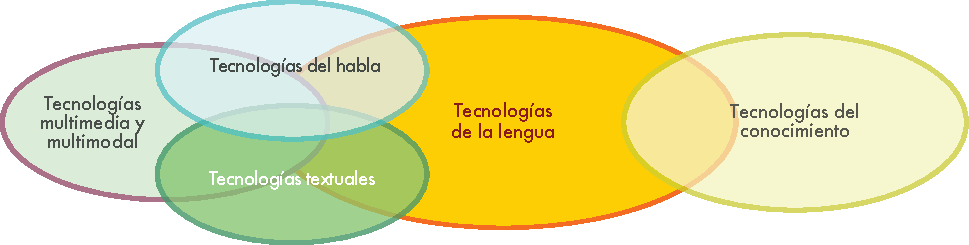
\includegraphics[width=\textwidth]{../_media/spanish/language_technologies}
  \caption{Tecnologías de la lengua}
  \label{fig:ltincontext_de}
  \colorrule{grey3}{\textwidth}{1.5pt}
\end{figure*}

En las siguientes secciones, discutiremos los principales ámbitos de aplicación de la tecnología lingüística: la corrección automática, la búsqueda en la Web, las tecnologías del habla y la traducción automática. Esto incluye aplicaciones y tecnologías básicas, como:

\begin{itemize}
  \item	corrección ortográfica
  \item	asistencia a la edición
  \item	aprendizaje de idiomas asistido por ordenador
  \item	recuperación de información
  \item	extracción de información
  \item	resumen de texto
  \item	búsqueda de respuestas
  \item	reconocimiento de voz
  \item	síntesis de voz
\end{itemize}

Antes de entrar en detalle en cada una de estas áreas, describiremos brevemente la arquitectura de un sistema de procesamiento típico. 

\subsection{Arquitectura de las aplicaciones}

Los diferentes módulos que constituyen las aplicaciones de procesamiento del lenguaje suelen reflejar los diferentes niveles de análisis lingüístico. La figura de la derecha muestra una arquitectura muy simplificada de un sistema de procesamiento de textos típico. Los tres primeros módulos gestionan la estructura y el significado del texto de entrada:

\begin{figure*}[b]
  \colorrule{grey3}{\textwidth}{1.5pt}
  \center
  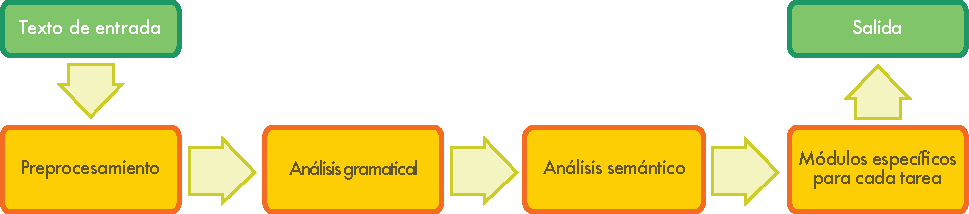
\includegraphics[width=\textwidth]{../_media/spanish/text_processing_app_architecture}
  \caption{Una arquitectura típica de aplicación de procesamiento de texto}
  \label{fig:textprocessingarch_de}
  \colorrule{grey3}{\textwidth}{1.5pt}
\end{figure*}

Tecnologías de la lengua es un área establecida de la investigación con un amplio conjunto de la literatura de introducción. El lector interesado puede consultar las siguientes referencias: \cite{jurafsky-martin01,manning-schuetze1,lt-world1,lt-survey1}.

\begin{enumerate}
  \item	Pre-procesamiento: limpia los datos, analiza o suprime el formato de entrada, detecta el idioma del texto, lo normaliza, etc.
  \item	Análisis gramatical: identificación del predicado y de sus argumentos, modificadores y otras partes del discurso, así como de la estructura de la oración.
  \item	Análisis semántico: desambigua (es decir, calcula el significado apropiado de las palabras en un contexto determinado), resuelve las anáforas (es decir, identifica los nombres a los que se refieren los pronombres en la oración), y representa el significado de la frase en una forma interpretable por la máquina.
\end{enumerate}

Después de analizar el texto, los módulos específicos pueden realizar otras operaciones, tales como resumen automático o consulta de bases de datos. Esta es una descripción simplificada e idealizada de la arquitectura típica de las aplicaciones lingüísticas y nos sirve para ilustrar la complejidad de estas.

Después de una breve introducción a cada una de las principales áreas de aplicación de las tecnologías lingüísticas, ofrecemos un breve resumen del estado de la investigación y de la educación en tecnología lingüística en España, y terminamos con un repaso de los programas de investigación, pasados y presentes. A continuación, presentamos una estimación experta de las herramientas y los recursos básicos del español según una diversidad de criterios, como por ejemplo, su disponibilidad, madurez y calidad. La situación general de las tecnologías lingüísticas en lengua española se resume en una tabla.

\subsection{Áreas principales de aplicación} 

En esta sección nos centramos en las herramientas y los recursos lingüísticos más importantes, y damos una visión general de las actividades de TL en España. 

\subsubsection{Corrección de textos}

Cualquiera que haya usado un procesador de texto como Microsoft Word sabe que tiene un corrector ortográfico que resalta los errores de ortografía y propone correcciones. Los primeros programas de corrección ortográfica comparaban cada palabra con un diccionario de palabras escritas correctamente. En la actualidad estos programas son mucho más sofisticados. Mediante algoritmos de análisis de texto, específicos para cada lengua, son capaces de detectar errores morfológicos (por ejemplo, la formación del plural), así como errores de sintaxis, tales como la falta de concordancia entre sujeto y verbo (por ejemplo, *ella escriben una carta). 

\begin{figure*}[htb]
  \colorrule{grey3}{\textwidth}{1.5pt}
  %\vspace{-9mm}
  \center
  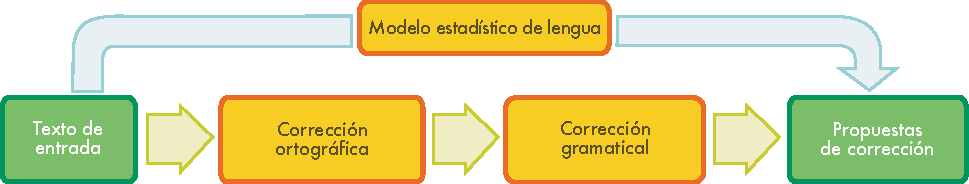
\includegraphics[width=\textwidth]{../_media/spanish/language_checking}
  \caption{Corrección de textos (parte superior: estadística; parte inferior: basada en reglas)}
  \label{fig:langcheckingaarch_de}
  \colorrule{grey3}{\textwidth}{1.5pt}
\end{figure*}

El tratamiento de muchos tipos de errores requiere un análisis del contexto. Un caso típico es cuando el error ortográfico transforma una palabra en otra palabra existente. En el siguiente ejemplo, la primera frase contiene un par de errores comunes (problemas con los acentos ortográficos y la omisión de /h/ muda). La segunda frase es la versión corregida de la primera:

\begin{quote}
  Mí calculo es que hoy a venido mas publico que ayer.\\
  Mi cálculo es que hoy ha venido más público que ayer.
\end{quote}

Para analizar el contexto lingüístico son necesarias reglas gramaticales laboriosamente codificadas por expertos, o bien un modelo de lenguaje estadístico construido a partir de corpus. En este último caso, el modelo calcula la probabilidad de que una palabra concreta aparezca en una posición específica (por ejemplo, entre las palabras que la preceden y la siguen). Por ejemplo, [Mi cálculo] o [ha venido] son secuencias de palabras mucho más probables que [Mí calculo] o [a venido] respectivamente. Un modelo estadístico de lenguaje se construye automáticamente a partir de una gran cantidad de texto (correcto), lo que se conoce como corpus textual. La mayor parte de las aplicaciones lingüísticas, ya sean basadas en reglas o en modelos estadísticos, se han desarrollado para el inglés. Otras lenguas han podido beneficiarse de toda la investigación realizada en torno al inglés. Sin embargo, no todos los tratamientos desarrollados para esta lengua se aplican bien a otras. Por ejemplo, los idiomas con una morfología más rica, o con un orden de palabras flexible, como el español, pueden necesitar un análisis lingüístico más profundo para alcanzar el mismo grado de precisión en la corrección de los textos.

La corrección de textos también se utiliza en sistemas de creación controlada de textos, es decir, entornos para la edición de manuales y documentación que siguen normas de escritura especiales, en el ámbito de la salud, ingeniería y otros. Para evitar reclamaciones sobre el uso incorrecto de sus aparatos o por daños resultantes de instrucciones mal entendidas, las empresas están insistiendo cada vez más en la calidad de la documentación técnica, y de las traducciones de sus versiones multilingües. Los avances en el procesamiento del lenguaje natural han llevado al desarrollo de software de edición que ayuda al autor de documentación técnica a usar vocabulario especializado y estructura de las frases compatibles con las normas de la industria y que se ajustan a las restricciones terminológicas corporativas.

Sólo una pocas empresas españolas ofrecen productos en este área. Por ejemplo, Daedalus, que nació como una spin-off de dos grupos de investigación de la Universidad Politécnica de Madrid (UPM) y de la Universidad Autónoma de Madrid (UAM), ha desarrollado STYLUS, un corrector ortográfico, gramatical y de estilo en español. La tecnología está disponible gratuitamente a través de su portal web, pero también puede integrarse en cualquier herramienta de gestión de contenidos. WinCorrect es un corrector ortográfico y gramatical desarrollado por Maxigramar (también con una versión en línea gratuita) y Signum es una PYME basada en Ecuador que desarrolló el corrector ortográfico para el español licenciado por Microsoft para Office.

Además de los correctores ortográficos y los servicios de edición, la tecnología de corrección de textos es también importante en el campo del aprendizaje de lenguas asistido por ordenador. Los motores de búsqueda, como Google, también utilizan correctores que corrigen de forma automática las consultas y proponen alternativas.

\subsubsection{Búsquedas en la Web}

Buscar en la Web, en las intranets o en las bibliotecas digitales es probablemente la aplicación de TL más utilizada en la actualidad. El motor de búsqueda de Google, que comenzó en 1998, ahora se encarga de aproximadamente del 80\% de todas las consultas. La interfaz de búsqueda de Google y la página donde muestra los resultados no han cambiado significativamente desde la primera versión. Sin embargo, en la versión actual, Google ofrece corrección de ortografía de las palabras mal escritas, y recientemente ha incorporado capacidades básicas de búsqueda semántica que pueden mejorar la precisión de la búsqueda mediante el análisis del significado de los términos de la consulta. El éxito de Google muestra que una gran cantidad de datos y unas técnicas eficientes de indexación pueden dar resultados satisfactorios, basados únicamente en métodos estadísticos.

\begin{figure*}[htb]
  \colorrule{grey3}{\textwidth}{1.5pt}
  %\vspace{-9mm}
  \center
  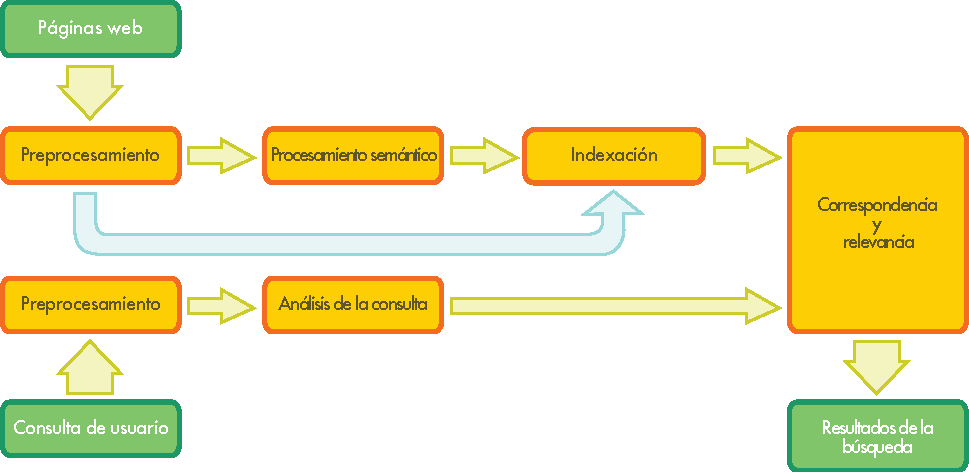
\includegraphics[width=\textwidth]{../_media/spanish/web_search_architecture}
  %\vspace{-5mm}
  \caption{Búsquedas en la web}
  \label{fig:websearcharch_de}
  \colorrule{grey3}{\textwidth}{1.5pt}
\end{figure*}

Para requerimientos de información más sofisticados, es esencial  integrar conocimiento lingüístico más complejo. El uso de recursos léxicos como tesauros (por ejemplo, WordNet) u ontologías aumenta la capacidad de búsqueda de páginas usando sinónimos de los términos originales, como por ejemplo "`Energía Atómica"' y "`Energía nuclear"', o incluso términos más vagamente relacionados.

La próxima generación de los motores de búsqueda tendrá que incluir tecnología lingüística mucho más sofisticada, con el fin de dar respuesta a las consultas que consisten en una pregunta o una petición, en lugar de una lista de palabras clave. Para la consulta, "`Dame una lista de todas las empresas que fueron adquiridas por otras compañías en los últimos cinco años,"' el sistema TL tiene que analizar la frase sintáctica y semánticamente, así como proporcionar un índice para recuperar rápidamente los documentos pertinentes. Una respuesta satisfactoria requieren un análisis sintáctico para analizar la estructura gramatical de la oración y determinar que el usuario quiere las compañías que han sido adquiridos, no las empresas que adquirieron otras empresas. Para la expresión “últimos cinco años”, el sistema necesita determinar los años pertinentes. Y, la consulta tiene que ser comparada con una enorme cantidad de datos no estructurados con objeto de encontrar la información relevante que el usuario desea. Esto se llama "`recuperación de información"', y consiste en la búsqueda y clasificación de los documentos pertinentes. Para generar una lista de empresas, el sistema también tiene que reconocer una secuencia particular de  palabras en un documento como nombres de empresa, un proceso llamado "`reconocimiento de entidades con nombre"'.

La recuperación de documentos en varios idiomas a partir de una única consulta en otro idioma distinto añade dificultad a la tarea. La recuperación de información multilingüe implica traducir automáticamente la consulta a todos los idiomas destino que sea posible y luego traducir los resultados de nuevo a la lengua origen.

Ahora que cada vez es más frecuente encontrar datos en formatos no textuales, se precisan servicios de recuperación de información multimedia que busquen imágenes, archivos de audio y de video. En el caso de archivos de audio y video, un módulo de reconocimiento de voz debe convertir el contenido de la voz en texto (o en una representación fonética) que pueda ser comparada con la consulta del usuario.

En España, unas pocas empresas desarrollan tecnología lingüística dirigida a la búsqueda y recuperación de información multilingüe, tanto desde Internet como desde sistemas de información internos. Entre las principales, se encuentran las siguientes: iSOCO, Dédalo, Inbenta, Bitext y Thera, esta última también spin-off, en este caso de la Universitat de Barcelona. Su tecnología incorpora herramientas de traducción automática, así como componentes de reconocimiento de entidades nombradas, búsqueda difusa y etiquetado semántico.

Estas empresas centran su desarrollo en el suministrar motores de búsqueda avanzados para portales de interés especial mediante el uso de semántica específica a un dominio. Debido a la gran demanda de potencia de procesamiento, estos motores de búsqueda sólo son eficientes en la gestión de corpus relativamente pequeños. El tiempo de procesamiento es varias miles de veces mayor que la que necesita un motor de búsqueda estándar estadístico como Google. Estos motores de búsqueda tienen una alta demanda para el modelado de dominio específico, pero no se pueden utilizar en la Web con sus miles y miles de millones de documentos.

\subsubsection{Procesamiento del habla}

La tecnología del procesamiento de voz se utiliza para crear interfaces que permiten a los usuarios interactuar a través de lengua hablada en lugar de una pantalla gráfica, teclado y ratón. Hoy en día, las interfaces de usuario de voz  se utilizan generalmente en los servicios de telefonía (semi-)automatizada proporcionada por las empresas a los clientes, empleados o socios. Los ámbitos comerciales que dependen en gran medida de este tipo de interfaces incluyen la banca, los suministros de servicios, el transporte público y las telecomunicaciones. Otros usos de la tecnología de voz incluyen interfaces para sistemas de navegación y el uso de la lengua oral como alternativa a las interfaces gráficas o la pantalla táctil de los smartphones.

\begin{figure*}[htb]
  \colorrule{grey3}{\textwidth}{1.5pt}
  \center  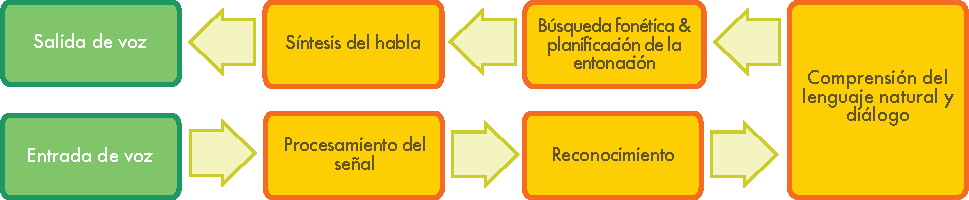
\includegraphics[width=\textwidth]{../_media/spanish/simple_speech-based_dialogue_architecture}
  \center
  \caption{Sistema de procesamiento del habla}
  \label{fig:dialoguearch_de}
  \colorrule{grey3}{\textwidth}{1.5pt}
\end{figure*}

Las tecnologías del habla comprenden las siguientes:

\begin{enumerate}
  \item El reconocimiento automático de voz, identifica las palabras a partir de una determinada secuencia de sonidos emitidos por un usuario.
  \item La comprensión del lenguaje natural, analiza la estructura sintáctica de la expresión de un usuario y lo interpreta de acuerdo con el sistema en cuestión.
  \item La gestión del diálogo, determina qué acción tomar, dada la entrada del usuario y la funcionalidad del sistema.
  \item La síntesis de voz (texto a voz) transforma la respuesta del sistema en sonidos para el usuario.
\end{enumerate}

Uno de los principales retos de los sistemas de reconocimiento es reconocer con precisión las palabras que un usuario emite. Esto implica restringir la gama de expresiones posibles de los usuarios a un conjunto limitado de palabras clave, o bien construir manualmente modelos de lenguaje que cubren una amplia gama de expresiones del lenguaje natural. Utilizando técnicas de aprendizaje automático, también se pueden generar modelos de lenguaje automáticamente a partir de corpus del habla, es decir,  de grandes colecciones de archivos de audio, acompañadas de transcripciones. Restringir la gama de expresiones por lo general obliga a los usuarios a utilizar una interfaz de voz de una manera rígida y puede no ser bien aceptado por el usuario, pero la creación y mantenimiento de modelos ricos de lengua aumenta significativamente los costos del sistema. 

Las empresas tienden a utilizar frases pregrabadas por locutores profesionales para generar la salida de la interfaz de usuario de voz. Para expresiones estáticas donde el texto no depende de los contextos particulares de uso o de los datos personales del usuario, esto puede ser suficiente. Pero en caso de contenidos más dinámicos, este sistema puede generar una entonación poco natural. Los sistemas actuales de texto a voz trabajan sobre este problema y son cada vez mejores en la producción de un sonido natural de expresiones generadas de forma dinámica por el sistema.

\boxtext{La tecnología del procesamiento de voz se utiliza para crear interfaces de lengua hablada.}

Las interfaces de voz que se hallan en el mercado, se han estandarizado considerablemente durante la última década, en términos de sus diversos componentes tecnológicos. También se ha consolidado el mercado en el reconocimiento y en la síntesis de voz. Los mercados nacionales de los países del G20 (países económicamente resistente con alta población) ha estado dominado por sólo cinco actores globales, con Nuance (EE.UU.) y Loquendo (Italia) entre los más importantes de Europa, también para el español, aunque algunas pequeñas compañías locales están empezando a competir, como Verbio, que es un spin-off de la Universitat Politècnica de Catalunya y dispone de tecnología de voz propia.

En cuanto a la tecnología de gestión de diálogo, los mercados están fuertemente dominados por actores nacionales, que suelen ser pequeñas empresas.

La mayoría de las empresas en el mercado español de las tecnologías de la voz son esencialmente desarrolladores de aplicaciones. Los principales actores en el mercado español son los siguientes: Indsys (Sistemas Inteligentes de diálogo), Fonetic , Ydilo y NaturalVoz. En lugar de depender de un modelo de negocio basado en las licencias de software, estas empresas se han posicionado principalmente como proveedores de servicios que crean interfaces de usuario de voz como parte de un servicio de integración de sistemas. En el área de la interacción del habla, no existe aún un mercado real para las tecnologías de análisis basadas en el análisi sintáctico y semántico.

La demanda de interfaces de voz en España ha crecido rápidamente en los últimos cinco años, impulsado por la creciente demanda de atención automática a los clientes, optimización de costes de los servicios telefónicos automatizados, y la creciente aceptación de la lengua oral como medio para la interacción hombre-máquina.

Mirando hacia el futuro, la propagación de los teléfonos inteligentes, o smartphones, como nueva plataforma para la gestión de relaciones con los clientes, además de la telefonía fija, Internet y correo electrónico, supondrá cambios significativos. Esto también afectará a como se usa la tecnología de voz. A la larga, el lenguaje hablado tendrá un papel mucho más importante como una entrada fácil de usar para los teléfonos inteligentes. Esto se deberá principalmente a mejoras en el reconocimiento de voz independiente de locutor, a través de servicios de dictado que ya se ofrecen como servicios centralizados a los usuarios de los smartphones. 

\subsubsection{Traducción Automática}

La idea de utilizar ordenadores para traducir de una lengua a otra se remonta a 1946 y la investigación en este ámbito gozó de una importante financiación durante la década de 1950 y de nuevo en la década de 1980. Sin embargo, la traducción automática (TA) aún no es capaz de cumplir su objetivo inicial de traducción automática de gran calidad e independiente de dominio.

\boxtext{La aproximación más simple a la traducción automática consiste en reemplazar automáticamente las palabras de un texto en un idioma, por palabras en otro idioma.}

La aproximación más simple a la traducción automática consiste en reemplazar automáticamente las palabras de un texto en un idioma, por palabras en otro idioma. Esto puede ser útil en ámbitos que tienen un lenguaje muy restringido, como los informes metorológicos. Sin embargo, para producir una buena traducción de textos menos estandarizados, hay que asociar unidades mayores de texto (sintagmas, oraciones, o incluso párrafos completos) con sus traducciones en la lengua destino. La mayor dificultad es que el lenguaje humano es ambiguo. La ambigüedad afecta múltiples niveles, por ejemplo la desambiguación de sentidos a nivel léxico (un jaguar es una marca de coche o un animal) o la asignación de casos a nivel sintáctico, por ejemplo:

\begin{itemize}
  \item[] \textit{The woman saw the car and her husband, too.}
  \item[] [La mujer vio el coche y su marido también.]
  \item[] [La mujer vio el coche y a su marido también.]
\end{itemize}

Una forma de construir un sistema de TA es escribir reglas lingüísticas. Los sistemas basados en reglas (o basados en conocimiento lingüístico) analizan el texto de entrada y crean una representación simbólica intermedia a partir de la cual puede generarse el texto en la lengua de destino. El éxito de estos métodos depende en gran medida de la disponibilidad de léxicos amplios con información morfológica, sintáctica y semántica, y de grandes conjuntos de reglas gramaticales cuidadosamente diseñadas por expertos lingüistas. Este es un proceso muy largo y costoso.

\begin{figure*}[htb]
  \colorrule{grey3}{\textwidth}{1.5pt}
  \center
  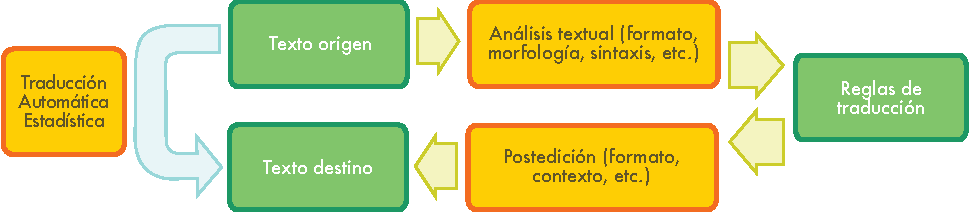
\includegraphics[width=\textwidth]{../_media/spanish/machine_translation}
  \caption{Traducción Automática (a la izquierda: estadística; a la derecha: basada en reglas)}
  \label{fig:mtarch_de}
  \colorrule{grey3}{\textwidth}{1.5pt}
\end{figure*}

A finales de 1980, cuando aumentó la potencia de cálculo de los ordenadores y se hizo más barata, creció el interés por la traducción automática basada en modelos estadísticos. Los modelos estadísticos se obtienen a partir del análisis de textos bilingües, como el corpus Europarl, que contiene las actas del Parlamento Europeo en 11 idiomas distintos. Si se cuenta con una cantidad suficiente de datos, la TA estadística (o basada en los datos) funciona lo suficientemente bien como para obtener una traducción aproximada de un texto mediante el procesamiento de versiones paralelas y la búsqueda de emparejamientos potenciales de palabras. Pero, a diferencia de los sistemas basados en conocimiento, la TA estadística a menudo genera resultados agramaticales. La TA estadística es ventajosa porque requiere menos esfuerzo humano, y también puede cubrir algunas particularidades de la lengua (por ejemplo, expresiones, idiomáticas) que suelen ser ignoradas por los sistemas basados en el conocimiento.

Las virtudes y los defectos de la TA basada en reglas y de la TA estadística tienden a ser complementarios, de modo que en la actualidad los investigadores se centran en enfoques híbridos que combinan ambas metodologías. Una posibilidad consiste en  utilizar los dos tipos de sistemas junto con un módulo de selección que decide sobre el mejor resultado para cada oración. Sin embargo, los resultados para las frases de más de 12 palabras no suelen ser buenos. Una solución mejor consiste en combinar las mejores traducciones de cada parte de la frase a partir de múltiples resultados, lo que puede resultar bastante complejo, ya que la segmentación y alineamiento de las distintas partes no suele ser obvia.

Lucy Software es una empresa internacional, líder en TA, que cuenta con una importante filial en España, Lucy Ibérica, anteriormente Translendium. Lucy Ibérica es responsable del desarrollo de los pares de idiomas que incluyen el español y todos los pares de idiomas que incluyen cualquier otra lengua ibérica (catalán, portugués, gallego y vasco). Word Magic es un conocido sistema de TA Español-Inglés (y viceversa) desarrollado por una empresa estadounidense. Tanto Lucy como Word Magic son sistemas basados en reglas gramticales. Si bien se investiga en sistemas de TA estadísticos e híbridos tanto en el contexto nacional como internacional, esta metodología ha tenido menos éxito en los negocios que en la investigación hasta el momento, con sólo unas pocas empresas que ofrece TA estadística adaptada al cliente, como Pangeanic.

Apertium es una plataforma de traducción automática, libre y de código abierto, que proporciona un motor de traducción, independiente de lengua, diseñado inicialmente por el grupo Transducens de la Universitat d'Alacant y, posteriormente, desarrollado en el marco del proyecto Opentrad , financiado con fondos nacionales. Entre los sistemas de traducción actuales que usan la tecnología Apertium, encontramos interNOSTRUM (español-catalán), Traductor Universia (español-portugués) y Matxin (euskera-español), los dos primeros desarrollados por Transducens y el tercero por el grupo IXA de la Euskal Herriko Unibertsitatea. Es posible usar Apertium para construir sistemas de traducción automática para una gran diversidad de combinaciones de idiomas (hay más de 20 hasta la fecha). Apertium usa formatos simples basados en XML para codificar los datos lingüísticos necesarios (ya sea a mano o por conversión de datos preexistentes), que se compilan utilizando las herramientas proporcionadas por el sistema y se convierten a los formatos de alta velocidad utilizado por el motor de traducción.

El uso de la traducción automática puede aumentar significativamente la productividad siempre que el sistema se adapte de forma inteligente a la terminología específica del usuario y se integre en un flujo de trabajo.
Todavía hay un enorme potencial para mejorar la calidad de los sistemas de MT. Los desafíos implican la adaptación de los recursos lingüísticos a un dominio determinado o área de usuario, y la integración de la tecnología en los flujos de trabajo que ya cuentan con bases terminológicas y las memorias de traducción. Otro problema es que la mayoría de los sistemas actuales están centrados en el inglés y  muy pocos proporcionan traducción entre el español y otras lenguas, distintas del inglés. 

Existen campañas de evaluación periódicas que ayudan a comparar la calidad de los sistemas de MT existentes y la cobertura de los distintos pares de idiomas. La tabla de abajo, que fue establecida en el proyecto de la CE Euromatrix +, muestra los resultados de los distintos pares para 22 de las 23 lenguas oficiales de la UE (el irlandés Gaélico no se comparó). Los resultados se clasifican de acuerdo a la métrica BLEU, que indica una puntuación más alta para una mejor traducción. (Un traductor humano alcanzaría una puntuación de unos 80 puntos.)

Los mejores resultados (en verde y azul) corresponden a las lenguas que se benefician de un mayor esfuerzo de investigación en programas coordinados y de la existencia de corpus paralelos (por ejemplo, inglés, francés, holandés, español y alemán). Los idiomas con los peores resultados (en rojo), o bien carecen de dichos esfuerzos de investigación, o bien se trata de idiomas tipológicamente muy distantes al resto (por ejemplo, húngaro, maltés y finés).

\begin{figure*}[tb]
  \centering
  \setlength{\tabcolsep}{0.17em}
  \small
  \begin{tabular}{>{\columncolor{corange1}}cccccccccccccccccccccccc}
    & \multicolumn{22}{>{\columncolor{corange1}}c}{Idioma de destino -- \textcolor{grey1}{Target language}}\\\addlinespace[{-.009cm}]
    \rowcolor{corange1}  & EN & BG & DE & CS & DA & EL & ES & ET & FI & FR & HU & IT & LT & LV & MT & NL & PL & PT & RO & SK & SL & SV\\
    EN & -- & \textcolor{blue}{40.5} & \textcolor{blue}{46.8} & \textcolor{green2}{52.6} & \textcolor{green2}{50.0} & \textcolor{blue}{41.0} & \textcolor{green2}{55.2} & \textcolor{purple}{34.8} & \textcolor{purple}{38.6} & \textcolor{green2}{50.1} & \textcolor{purple}{37.2} & \textcolor{green2}{50.4} & \textcolor{purple}{39.6} & \textcolor{blue}{43.4} & \textcolor{purple}{39.8} & \textcolor{green2}{52.3} & \textcolor{blue}{49.2} & \textcolor{green2}{55.0} & \textcolor{blue}{49.0} & \textcolor{blue}{44.7} & \textcolor{green2}{50.7} & \textcolor{green2}{52.0}\\
    BG & \textcolor{green}{61.3} & -- & \textcolor{purple}{38.7} & \textcolor{purple}{39.4} & \textcolor{purple}{39.6} & \textcolor{purple}{34.5} & \textcolor{blue}{46.9} & \textcolor{red3}{25.5} & \textcolor{red3}{26.7} & \textcolor{blue}{42.4} & \textcolor{red3}{22.0} & \textcolor{blue}{43.5} & \textcolor{red3}{29.3} & \textcolor{red3}{29.1} & \textcolor{red3}{25.9} & \textcolor{blue}{44.9} & \textcolor{purple}{35.1} & \textcolor{blue}{45.9} & \textcolor{purple}{36.8} & \textcolor{purple}{34.1} & \textcolor{purple}{34.1} & \textcolor{purple}{39.9}\\
    DE & \textcolor{green2}{53.6} & \textcolor{red3}{26.3} & -- & \textcolor{purple}{35.4} & \textcolor{blue}{43.1} & \textcolor{purple}{32.8} & \textcolor{blue}{47.1} & \textcolor{red3}{26.7} & \textcolor{red3}{29.5} & \textcolor{purple}{39.4} & \textcolor{red3}{27.6} & \textcolor{blue}{42.7} & \textcolor{red3}{27.6} & \textcolor{purple}{30.3} & \textcolor{red2}{19.8} & \textcolor{green2}{50.2} & \textcolor{purple}{30.2} & \textcolor{blue}{44.1} & \textcolor{purple}{30.7} & \textcolor{red3}{29.4} & \textcolor{purple}{31.4} & \textcolor{blue}{41.2}\\
    CS & \textcolor{green2}{58.4} & \textcolor{purple}{32.0} & \textcolor{blue}{42.6} & -- & \textcolor{blue}{43.6} & \textcolor{purple}{34.6} & \textcolor{blue}{48.9} & \textcolor{purple}{30.7} & \textcolor{purple}{30.5} & \textcolor{blue}{41.6} & \textcolor{red3}{27.4} & \textcolor{blue}{44.3} & \textcolor{purple}{34.5} & \textcolor{purple}{35.8} & \textcolor{red3}{26.3} & \textcolor{blue}{46.5} & \textcolor{purple}{39.2} & \textcolor{blue}{45.7} & \textcolor{purple}{36.5} & \textcolor{blue}{43.6} & \textcolor{blue}{41.3} & \textcolor{blue}{42.9}\\
    DA & \textcolor{green2}{57.6} & \textcolor{red3}{28.7} & \textcolor{blue}{44.1} & \textcolor{purple}{35.7} & -- & \textcolor{purple}{34.3} & \textcolor{blue}{47.5} & \textcolor{red3}{27.8} & \textcolor{purple}{31.6} & \textcolor{blue}{41.3} & \textcolor{red3}{24.2} & \textcolor{blue}{43.8} & \textcolor{red3}{29.7} & \textcolor{purple}{32.9} & \textcolor{red3}{21.1} & \textcolor{blue}{48.5} & \textcolor{purple}{34.3} & \textcolor{blue}{45.4} & \textcolor{purple}{33.9} & \textcolor{purple}{33.0} & \textcolor{purple}{36.2} & \textcolor{blue}{47.2}\\
    EL & \textcolor{green2}{59.5} & \textcolor{purple}{32.4} & \textcolor{blue}{43.1} & \textcolor{purple}{37.7} & \textcolor{blue}{44.5} & -- & \textcolor{green2}{54.0} & \textcolor{red3}{26.5} & \textcolor{red3}{29.0} & \textcolor{blue}{48.3} & \textcolor{red3}{23.7} & \textcolor{blue}{49.6} & \textcolor{red3}{29.0} & \textcolor{purple}{32.6} & \textcolor{red3}{23.8} & \textcolor{blue}{48.9} & \textcolor{purple}{34.2} & \textcolor{green2}{52.5} & \textcolor{purple}{37.2} & \textcolor{purple}{33.1} & \textcolor{purple}{36.3} & \textcolor{blue}{43.3}\\
    ES & \textcolor{green}{60.0} & \textcolor{purple}{31.1} & \textcolor{blue}{42.7} & \textcolor{purple}{37.5} & \textcolor{blue}{44.4} & \textcolor{purple}{39.4} & -- & \textcolor{red3}{25.4} & \textcolor{red3}{28.5} & \textcolor{green2}{51.3} & \textcolor{red3}{24.0} & \textcolor{green2}{51.7} & \textcolor{red3}{26.8} & \textcolor{purple}{30.5} & \textcolor{red3}{24.6} & \textcolor{blue}{48.8} & \textcolor{purple}{33.9} & \textcolor{green2}{57.3} & \textcolor{purple}{38.1} & \textcolor{purple}{31.7} & \textcolor{purple}{33.9} & \textcolor{blue}{43.7}\\
    ET & \textcolor{green2}{52.0} & \textcolor{red3}{24.6} & \textcolor{purple}{37.3} & \textcolor{purple}{35.2} & \textcolor{purple}{37.8} & \textcolor{red3}{28.2} & \textcolor{blue}{40.4} & -- & \textcolor{purple}{37.7} & \textcolor{purple}{33.4} & \textcolor{purple}{30.9} & \textcolor{purple}{37.0} & \textcolor{purple}{35.0} & \textcolor{purple}{36.9} & \textcolor{red3}{20.5} & \textcolor{blue}{41.3} & \textcolor{purple}{32.0} & \textcolor{purple}{37.8} & \textcolor{red3}{28.0} & \textcolor{purple}{30.6} & \textcolor{purple}{32.9} & \textcolor{purple}{37.3}\\
    FI & \textcolor{blue}{49.3} & \textcolor{red3}{23.2} & \textcolor{purple}{36.0} & \textcolor{purple}{32.0} & \textcolor{purple}{37.9} & \textcolor{red3}{27.2} & \textcolor{purple}{39.7} & \textcolor{purple}{34.9} & -- & \textcolor{red3}{29.5} & \textcolor{red3}{27.2} & \textcolor{purple}{36.6} & \textcolor{purple}{30.5} & \textcolor{purple}{32.5} & \textcolor{red2}{19.4} & \textcolor{blue}{40.6} & \textcolor{red3}{28.8} & \textcolor{purple}{37.5} & \textcolor{red3}{26.5} & \textcolor{red3}{27.3} & \textcolor{red3}{28.2} & \textcolor{purple}{37.6}\\
    FR & \textcolor{green}{64.0} & \textcolor{purple}{34.5} & \textcolor{blue}{45.1} & \textcolor{purple}{39.5} & \textcolor{blue}{47.4} & \textcolor{blue}{42.8} & \textcolor{green}{60.9} & \textcolor{red3}{26.7} & \textcolor{purple}{30.0} & -- & \textcolor{red3}{25.5} & \textcolor{green2}{56.1} & \textcolor{red3}{28.3} & \textcolor{purple}{31.9} & \textcolor{red3}{25.3} & \textcolor{green2}{51.6} & \textcolor{purple}{35.7} & \textcolor{green}{61.0} & \textcolor{blue}{43.8} & \textcolor{purple}{33.1} & \textcolor{purple}{35.6} & \textcolor{blue}{45.8}\\
    HU & \textcolor{blue}{48.0} & \textcolor{red3}{24.7} & \textcolor{purple}{34.3} & \textcolor{purple}{30.0} & \textcolor{purple}{33.0} & \textcolor{red3}{25.5} & \textcolor{purple}{34.1} & \textcolor{red3}{29.6} & \textcolor{red3}{29.4} & \textcolor{purple}{30.7} & -- & \textcolor{purple}{33.5} & \textcolor{red3}{29.6} & \textcolor{purple}{31.9} & \textcolor{red2}{18.1} & \textcolor{purple}{36.1} & \textcolor{red3}{29.8} & \textcolor{purple}{34.2} & \textcolor{red3}{25.7} & \textcolor{red3}{25.6} & \textcolor{red3}{28.2} & \textcolor{purple}{30.5}\\
    IT & \textcolor{green}{61.0} & \textcolor{purple}{32.1} & \textcolor{blue}{44.3} & \textcolor{purple}{38.9} & \textcolor{blue}{45.8} & \textcolor{blue}{40.6} & \textcolor{red3}{26.9} & \textcolor{red3}{25.0} & \textcolor{red3}{29.7} & \textcolor{green2}{52.7} & \textcolor{red3}{24.2} & -- & \textcolor{red3}{29.4} & \textcolor{purple}{32.6} & \textcolor{red3}{24.6} & \textcolor{green2}{50.5} & \textcolor{purple}{35.2} & \textcolor{green2}{56.5} & \textcolor{purple}{39.3} & \textcolor{purple}{32.5} & \textcolor{purple}{34.7} & \textcolor{blue}{44.3}\\
    LT & \textcolor{green2}{51.8} & \textcolor{red3}{27.6} & \textcolor{purple}{33.9} & \textcolor{purple}{37.0} & \textcolor{purple}{36.8} & \textcolor{red3}{26.5} & \textcolor{red3}{21.1} & \textcolor{purple}{34.2} & \textcolor{purple}{32.0} & \textcolor{purple}{34.4} & \textcolor{red3}{28.5} & \textcolor{purple}{36.8} & -- & \textcolor{blue}{40.1} & \textcolor{red3}{22.2} & \textcolor{purple}{38.1} & \textcolor{purple}{31.6} & \textcolor{purple}{31.6} & \textcolor{red3}{29.3} & \textcolor{purple}{31.8} & \textcolor{purple}{35.3} & \textcolor{purple}{35.3}\\
    LV & \textcolor{green2}{54.0} & \textcolor{red3}{29.1} & \textcolor{purple}{35.0} & \textcolor{purple}{37.8} & \textcolor{purple}{38.5} & \textcolor{red3}{29.7} & \textcolor{red2}{8.0} & \textcolor{purple}{34.2} & \textcolor{purple}{32.4} & \textcolor{purple}{35.6} & \textcolor{red3}{29.3} & \textcolor{purple}{38.9} & \textcolor{purple}{38.4} & -- & \textcolor{red3}{23.3} & \textcolor{blue}{41.5} & \textcolor{purple}{34.4} & \textcolor{purple}{39.6} & \textcolor{purple}{31.0} & \textcolor{purple}{33.3} & \textcolor{purple}{37.1} & \textcolor{purple}{38.0}\\
    MT & \textcolor{green}{72.1} & \textcolor{purple}{32.2} & \textcolor{purple}{37.2} & \textcolor{purple}{37.9} & \textcolor{purple}{38.9} & \textcolor{purple}{33.7} & \textcolor{blue}{48.7} & \textcolor{red3}{26.9} & \textcolor{red3}{25.8} & \textcolor{blue}{42.4} & \textcolor{red3}{22.4} & \textcolor{blue}{43.7} & \textcolor{purple}{30.2} & \textcolor{purple}{33.2} & -- & \textcolor{blue}{44.0} & \textcolor{purple}{37.1} & \textcolor{blue}{45.9} & \textcolor{purple}{38.9} & \textcolor{purple}{35.8} & \textcolor{blue}{40.0} & \textcolor{blue}{41.6}\\
    NL & \textcolor{green2}{56.9} & \textcolor{red3}{29.3} & \textcolor{blue}{46.9} & \textcolor{purple}{37.0} & \textcolor{blue}{45.4} & \textcolor{purple}{35.3} & \textcolor{blue}{49.7} & \textcolor{red3}{27.5} & \textcolor{red3}{29.8} & \textcolor{blue}{43.4} & \textcolor{red3}{25.3} & \textcolor{blue}{44.5} & \textcolor{red3}{28.6} & \textcolor{purple}{31.7} & \textcolor{red3}{22.0} & -- & \textcolor{purple}{32.0} & \textcolor{blue}{47.7} & \textcolor{purple}{33.0} & \textcolor{purple}{30.1} & \textcolor{purple}{34.6} & \textcolor{blue}{43.6}\\
    PL & \textcolor{green}{60.8} & \textcolor{purple}{31.5} & \textcolor{blue}{40.2} & \textcolor{blue}{44.2} & \textcolor{blue}{42.1} & \textcolor{purple}{34.2} & \textcolor{blue}{46.2} & \textcolor{red3}{29.2} & \textcolor{red3}{29.0} & \textcolor{blue}{40.0} & \textcolor{red3}{24.5} & \textcolor{blue}{43.2} & \textcolor{purple}{33.2} & \textcolor{purple}{35.6} & \textcolor{red3}{27.9} & \textcolor{blue}{44.8} & -- & \textcolor{blue}{44.1} & \textcolor{purple}{38.2} & \textcolor{purple}{38.2} & \textcolor{purple}{39.8} & \textcolor{blue}{42.1}\\
    PT & \textcolor{green}{60.7} & \textcolor{purple}{31.4} & \textcolor{blue}{42.9} & \textcolor{purple}{38.4} & \textcolor{blue}{42.8} & \textcolor{blue}{40.2} & \textcolor{green}{60.7} & \textcolor{red3}{26.4} & \textcolor{red3}{29.2} & \textcolor{green2}{53.2} & \textcolor{red3}{23.8} & \textcolor{green2}{52.8} & \textcolor{red3}{28.0} & \textcolor{purple}{31.5} & \textcolor{red3}{24.8} & \textcolor{blue}{49.3} & \textcolor{purple}{34.5} & -- & \textcolor{purple}{39.4} & \textcolor{purple}{32.1} & \textcolor{purple}{34.4} & \textcolor{blue}{43.9}\\
    RO & \textcolor{green}{60.8} & \textcolor{purple}{33.1} & \textcolor{purple}{38.5} & \textcolor{purple}{37.8} & \textcolor{blue}{40.3} & \textcolor{purple}{35.6} & \textcolor{green2}{50.4} & \textcolor{red3}{24.6} & \textcolor{red3}{26.2} & \textcolor{blue}{46.5} & \textcolor{red3}{25.0} & \textcolor{blue}{44.8} & \textcolor{red3}{28.4} & \textcolor{red3}{29.9} & \textcolor{red3}{28.7} & \textcolor{blue}{43.0} & \textcolor{purple}{35.8} & \textcolor{blue}{48.5} & -- & \textcolor{purple}{31.5} & \textcolor{purple}{35.1} & \textcolor{purple}{39.4}\\
    SK & \textcolor{green}{60.8} & \textcolor{purple}{32.6} & \textcolor{purple}{39.4} & \textcolor{blue}{48.1} & \textcolor{blue}{41.0} & \textcolor{purple}{33.3} & \textcolor{blue}{46.2} & \textcolor{red3}{29.8} & \textcolor{red3}{28.4} & \textcolor{purple}{39.4} & \textcolor{red3}{27.4} & \textcolor{blue}{41.8} & \textcolor{purple}{33.8} & \textcolor{purple}{36.7} & \textcolor{red3}{28.5} & \textcolor{blue}{44.4} & \textcolor{purple}{39.0} & \textcolor{blue}{43.3} & \textcolor{purple}{35.3} & -- & \textcolor{blue}{42.6} & \textcolor{blue}{41.8}\\
    SL & \textcolor{green}{61.0} & \textcolor{purple}{33.1} & \textcolor{purple}{37.9} & \textcolor{blue}{43.5} & \textcolor{blue}{42.6} & \textcolor{purple}{34.0} & \textcolor{blue}{47.0} & \textcolor{purple}{31.1} & \textcolor{red3}{28.8} & \textcolor{purple}{38.2} & \textcolor{red3}{25.7} & \textcolor{blue}{42.3} & \textcolor{purple}{34.6} & \textcolor{purple}{37.3} & \textcolor{purple}{30.0} & \textcolor{blue}{45.9} & \textcolor{purple}{38.2} & \textcolor{blue}{44.1} & \textcolor{purple}{35.8} & \textcolor{purple}{38.9} & -- & \textcolor{blue}{42.7}\\
    SV & \textcolor{green2}{58.5} & \textcolor{red3}{26.9} & \textcolor{blue}{41.0} & \textcolor{purple}{35.6} & \textcolor{blue}{46.6} & \textcolor{purple}{33.3} & \textcolor{blue}{46.6} & \textcolor{red3}{27.4} & \textcolor{purple}{30.9} & \textcolor{purple}{38.9} & \textcolor{red3}{22.7} & \textcolor{blue}{42.0} & \textcolor{red3}{28.2} & \textcolor{purple}{31.0} & \textcolor{red3}{23.7} & \textcolor{blue}{45.6} & \textcolor{purple}{32.2} & \textcolor{blue}{44.2} & \textcolor{purple}{32.7} & \textcolor{purple}{31.3} & \textcolor{purple}{33.5} & --\\
    \end{tabular}
  \caption{Rendimiento de los sistemas de Traducción Automática para los pares de lenguas del proyecto Euromatrix+ -- \textcolor{grey1}{Machine translation between 22 EU-languages \cite{euro1}}}
  \label{fig:euromatrix_es}
\end{figure*}

\subsection{Otras áreas de aplicación}

La construcción de aplicaciones lingüísticas implica un conjunto de tecnologías que no siempre aparecen de forma evidente en el nivel de interacción con el usuario, pero que proporcionan funcionalidades importantes al sistema en cuestión. Todos ellos constituyen temas importantes de investigación que han evolucionado hasta convertirse en sub-disciplinas específicas de la lingüística computacional.

\boxtext{Las tecnologías lingüísticas proporcionan funcionalidades importantes de forma no siempre evidente.}

La \textbf{búsqueda de respuestas} o question answering, por ejemplo, es un área activa de investigación para la que se han construido corpus anotados y se han puesto en marcha concursos científicos. El concepto de búsqueda de respuestas va más allá de las búsquedas convencionales basadas en palabras clave (en las que el motor de búsqueda responde mediante la entrega de una colección de documentos potencialmente relevantes). Este tipo de búsqueda permite a los usuarios hacer una pregunta concreta a la que el sistema proporciona una respuesta única. Por ejemplo:

\begin{itemize}
  \item[] \textit{Pregunta: ¿Qué edad tenía Neil Armstrong cuando pisó la luna?}
  \item[] \textit{Respuesta: 38.}
\end{itemize}

A pesar de que la búsqueda de respuestas está obviamente relacionada con la búsqueda en la Web, hoy en día es un término general que engloba temas de investigación tales como: qué tipos de preguntas hay y cómo deberían tratarse; cómo pueden analizarse y compararse un conjunto de documentos que podrían contener la respuesta (¿ofrecen respuestas contradictorias?), y cómo puede extraerse de forma fiable la información específica (es decir, la respuesta) de un documento sin descuidar el contexto. 

Esto a su vez está relacionado con la \textbf{extracción de información}, un ámbito que se hizo muy popular e influyente cuando la lingüística computacional dio un giro hacia la estadística en la década de 1990. La extracción de información tiene como objetivo identificar información específica en clases de documentos específicos, como por ejemplo, la detección de los actores clave en la adquisición de empresas a partir de informaciones periodísticas. Otra situación común que se ha estudiado son los informes sobre incidentes terroristas. El problema aquí consiste en proyectar el texto hacia una plantilla que especifique el autor, el objetivo, hora, lugar y los resultados del incidente. La extracción de información consiste básicamente en llenar plantillas relativas a dominios específicos, por lo que constituye otro ejemplo de tecnología “entre bastidores” que en la práctica tiene que ser integrada en un entorno de aplicación adecuada. 

El \textbf{resumen} y la \textbf{generación de texto} son dos ámbitos muy relacionados que pueden actuar como aplicaciones independientes o desempeñar un papel de apoyo „entre bastidores”. El resumen de textos intenta dar los elementos esenciales de un texto largo de una forma breve, y es una de las funcionalidades disponibles en Microsoft Word. Utiliza principalmente métodos estadísticos para identificar las palabras „importantes” de un texto (es decir, palabras que son muy frecuentes en el texto en cuestión, pero menos frecuentes en el uso del lenguaje en general) y determinar así qué frases contienen la mayor parte de estas palabras „importantes”. Estas frases luego se extraen y combinan para crear el resumen. En este escenario comercial, muy común, el resumen es simplemente una forma de extracción de frases, y el texto se reduce a un subconjunto de las mismas. Un enfoque alternativo, que también se ha investigado, consiste en generar oraciones completamente nuevas  que no existían en el texto original. Esto requiere una comprensión más profunda del texto, lo que significa que hasta el momento este enfoque es mucho menos robusto. En general, un generador de texto rara vez se utiliza como una aplicación independiente, sino que se integra en un entorno de software más grande, como, por ejemplo, un sistema de información clínica que recoge, almacena y procesa los datos de los pacientes. La creación de informes es sólo una de las muchas aplicaciones del resumen de texto.

\boxtext{La investigación en estas tecnologías está mucho menos desarro-llada para la lengua española que para el inglés.} 

La investigación en estas tecnologías está mucho menos desarrollada para la lengua española que para el inglés. La búsqueda de respuestas, la extracción de información y el resumen han sido objeto de numerosas competiciones en los EE.UU. desde la década de 1990, organizados principalmente por las organizaciones gubernamentales DARPA y NIST. Estas competiciones han mejorado significativamente el nivel de las tecnologías, pero se han centrado sobre todo en el inglés. Como resultado, casi no hay corpus anotado u otros recursos especiales necesarios para realizar estas tareas en español. Los sistemas de resumen que utilizan métodos puramente estadísticos son en gran parte independientes de idioma y existe una serie de prototipos de investigación disponibles. En la generación de texto, los componentes reutilizables se han limitado en general a los módulos de realización de superficie (gramáticas de generación) y la mayor parte del software disponible es para inglés.

Aparte de los sistemas experimentales que desarrollan los grupos de investigación, hay algunas empresas que ofrecen este tipo de servicios. Entre ellas, Daedalus e Inbenta, y algunas empresas internacionales con una presencia significativa en el mercado español, como Q-go y Artificial Solutions.

\subsection{Programas Educativos}

La tecnología lingüística es un campo altamente interdisciplinario, que involucra la experiencia de lingüistas, informáticos, matemáticos, filósofos, psicolingüistas, y neurólogos, entre otros. En consecuencia, la formación básica actual de un lingüística computacional puede ser realizada en España en el marco de una licenciatura en Filología o Lingüística, que incluyen como asignatura troncal Lingüística Computacional, o bien en el de una ingeniería informática. Entre las universidades que ofrecen la primera opción: Universitat de Barcelona, Universitat Pompeu Fabra, Universitat Oberta de Catalunya y la Universidad de Vigo. Por otro lado, las principales ingenierías que ofrecen lingüística computacional como asignatura están en: Universidad Politécnica de Madrid, Universidad Carlos III, Universidad Autónoma de Madrid, Universitat d'Alacant, Universidad Nacional de Educación a Distancia, y Euskal Herriko Unibertsitatea. Otros casos, tales como la Universidad Complutense  combina ambas opciones.

Los cursos de posgrado ofrecen una formación profesional más específica. Hay varios programas de doctorado que ofrecen másters o asignaturas relacionados con el lenguaje y el procesamiento del habla. Algunas universidades como la Universitat Politècnica de Catalunya también participan en el Máster Europeo en Lengua y  Habla patrocinado por ELSNET (Red Europea de Excelencia en tecnologías del lenguaje humano). Los másters a menudo se ofrecen de forma colectiva, por un grupo de universidades, ya sea a nivel estatal o a nivel europeo. Por ejemplo, la Universitat Autònoma de Barcelona ofrece el Máster Internacional en Procesamiento del Lenguaje Natural y Tecnologías del Lenguaje Humano, en colaboración con universidades extranjeras. También se ofrecen módulos de Tecnología Lingüística a los estudiantes de otros masters o cursos de doctorado, sobre todo en traducción (por ejemplo, en la Autònoma de Barcelona, Alacant, Castelló, Politécnica de Valencia y Granada).

Hay más de 30 grupos de investigación en España, repartidos entre las diferentes universidades, que trabajan en el reconocimiento del habla, el procesamiento del lenguaje natural, la traducción de texto a texto y la síntesis de voz. La Sociedad Española para el Procesamiento del Lenguaje Natural, es una organización sin ánimo de lucro con más de 300 miembros, procedentes tanto del mundo académico como de la industria, que fue creada en 1984 con el objetivo de fomentar y difundir las actividades relacionados con la docencia, la investigación y el desarrollo del PLN, a nivel nacional e internacional. La SEPLN organiza seminarios, simposios y conferencias y promueve la colaboración entre instituciones nacionales e internacionales.

La SEPLN organiza una conferencia anual a la que asisten un número creciente de investigadores que trabajan en el  PLN, tanto en España como en el extranjero. La asociación edita una revista periódica y mantiene un servidor web con información sobre temas relacionados con el procesamiento del lenguaje natural y un foro abierto para los miembros de la asociación. 

\subsection{Proyectos e iniciativas nacionales}

El Ministerio de Educación, a través de la Comisión Interministerial de Ciencia y Tecnología (CICYT), que es el órgano que coordina y supervisa los planes estratégicos nacionales para la Ciencia y la Tecnología en España, apoya la investigación en el campo de las tecnologías de la información, a través de programas nacionales de investigación. Estos programas han impulsado numerosos proyectos de investigación y de colaboración con empresas y centros internacionales de investigación. La base del desarrollo tecnológico y de las aplicaciones comerciales para el procesamiento automático de la lengua española ha surgido en parte como resultado de estos proyectos.

El Centro para el Desarrollo Tecnológico Industrial (CDTI) es una organización pública española, dependiente del Ministerio de Ciencia e Innovación, cuyo objetivo es ayudar a las empresas españolas a incrementar su perfil tecnológico. El CDTI evalúa y financia proyectos I + D a través de programas como CENIT, AVANZA e INNPACTO.

El programa CENIT (Consorcios Estratégicos Nacionales para la Investigación Tecnológica) tiene como objetivo estimular la cooperación en I + D entre el sector privado, las universidades, los organismos y centros públicos de investigación, los parques científicos y los centros tecnológicos, impulsando la cooperación en I + D entre los sectores público y privado. Los proyectos CENIT tienen una duración mínima de cuatro años, un presupuesto mínimo de 5 millones de euros por año, y reciben una financiación mínima del 50\% del sector privado. Al menos el 50\% de la financiación pública se destina a centros públicos de investigación o a centros tecnológicos. Las tecnologías de la Información y la Comunicación son una de las áreas prioritarias del programa. Los proyectos en este área incluyen a menudo algún tipo de investigación en tecnologías del lenguaje.

El objetivo de los planes AVANZ@ e INNPACTO es acercar la Sociedad de la Información a los ciudadanos comunes, y a los sectores público y privado. Promover el uso de las TIC ha de tener un efecto en cadena sobre el conjunto del sector en España, y por consiguiente, en su carácter innovador. Los objetivos del Plan incluyen el incremento del porcentaje de empresas que utilizan el comercio electrónico; la promoción del uso de la facturación electrónica; la  implementación de un carnet de identidad electrónico y la extensión de los trámites públicos electrónicos; alcanzar la tasa de un ordenador conectado a Internet por cada dos alumnos en las escuelas; y duplicar el número de hogares con acceso a Internet. Entre sus mayores prioridades está el facilitar el uso de las nuevas tecnologías a las personas mayores y a las personas con discapacidad, como un medio ideal para lograr la integración social, evitar la exclusión y mejorar su calidad de vida. Las herramientas basadas en tecnología lingüística constituyen el medio principal para satisfacer este objetivo  (por ejemplo, los asistentes de lectura para ciegos que utilizan síntesis de voz).

Proyectos y programas anteriores han contribuido al desarrollo de una serie de herramientas de tecnología lingüística y de recursos para el español. En la siguiente sección, se resume el estado actual del soporte a la tecnología lingüística para el español.  

\subsection{Disponibilidad de herramientas y recursos}

La siguiente tabla resume el estado actual del soporte a la tecnología lingüística para el español. La evaluación de los instrumentos y los recursos existentes se basa en estimaciones proporcionadas por un grupo de expertos en cada área.

\begin{figure*}[htb]
  \centering
\begin{tabular}{>{\columncolor{orange1}}p{.33\linewidth}@{\hspace*{6mm}}c@{\hspace*{6mm}}c@{\hspace*{6mm}}c@{\hspace*{6mm}}c@{\hspace*{6mm}}c@{\hspace*{6mm}}c@{\hspace*{6mm}}c}
  \rowcolor{orange1}
   \cellcolor{white}&\begin{sideways}\makecell[l]{Cantidad}\end{sideways}
  &\begin{sideways}\makecell[l]{\makecell[l]{Disponibilidad} }\end{sideways} &\begin{sideways}\makecell[l]{Calidad}\end{sideways}
  &\begin{sideways}\makecell[l]{Cobertura}\end{sideways} &\begin{sideways}\makecell[l]{Madurez}\end{sideways} &\begin{sideways}\makecell[l]{Sostenibilidad}\end{sideways} &\begin{sideways}\makecell[l]{Adaptabilidad~~~}\end{sideways} \\ \addlinespace
  \multicolumn{8}{>{\columncolor{orange2}}l}{Tecnoligías lingüísticas: herramientas, tecnologías y aplicaciones} \\\addlinespace
  Reconocimiento de voz &2&3&4&2&2&2&4 \\ \addlinespace
  Síntesis de voz &3&3&4&4&4&3&4\\ \addlinespace
  Análisis gramatical &3&3&4&4&4.5&2.5&4.5\\ \addlinespace
  Análisis semántico &1.5&2&3&2&2.5&2.5&2.5\\ \addlinespace
  Generación de texto &0&0&0&0&0&0&0\\ \addlinespace
  Traducción automática &3&2&2&2&4&2&2\\ \addlinespace
  \multicolumn{8}{>{\columncolor{orange2}}l}{Recursos lingüísticos: recursos, datos y bases de conocimiento} \\\addlinespace
  Corpus textuales &3&3&4&4.5&4&4.5&4.5\\ \addlinespace
  Corpus de discurso &4&2&4&4&4&3&3\\ \addlinespace
  Corpus paralelos &2&4&2&2&2&3&3\\ \addlinespace
  Recursos léxicos &3.5&3&4.5&3&4&3&3\\ \addlinespace
  Gramáticas &1&4&5&2&2&2&2\\
  \end{tabular}
  \caption{Soporte a la tecnología lingüística para el español}
  \label{fig:lrlttable_de}
\end{figure*}

Los datos contenidos en esta tabla se pueden interpretar de forma resumida, de la siguiente manera:

\begin{itemize}
  \item El procesamiento del habla aparece como una tecnología ligeramente más madura que el procesamiento del texto escrito. De hecho, esta tecnología ya ha sido integrada con éxito en muchas aplicaciones cotidianas, como, por ejemplo, los sistemas de diálogo hablado y las interfaces de voz para móviles y navegadores para automóviles.
  \item La investigación realizada hasta la fecha, ha conducido con éxito al diseño de software de calidad media-alta para el análisis de textos básicos, tales como herramientas de análisis morfológicos y de análisis sintáctico. Sin embargo, las tecnologías que requieren un procesamiento lingüístico profundo y un conocimiento semántico, son todavía muy incipientes.
  \item En cuanto a los recursos, existe un corpus textual de referencia de gran tamaño para el español, que contiene una mezcla equilibrada de géneros, pero que no es de fácil acceso para la investigación. Existen también diversos corpus anotados con información sintáctica, semántica y de discurso, pero no son suficientes, ni en riqueza de anotaciones ni en tamaño, para satisfacer la creciente necesidad de información lingüística.
  \item En particular, hay una carencia de corpus paralelos que constituyen la base de los sistemas de traducción automática estadísticos e híbridos. Existen corpus paralelos entre el español y el inglés, así como entre el español y el resto de lenguas oficiales en España. Sin embargo, faltan corpus paralelos entre el español y otros idiomas.
  \item Muchas de estas herramientas, recursos y formatos de codificación no se ajustan a los estándares del sector y no se pueden mantener de forma eficaz. Se requiere un plan concertado para estandarizar las interfaces de las aplicaciones y los formatos de los datos.
  \item Existe una situación legal confusa que restringe la utilización de textos digitales, como las publicaciones en línea, para su uso en investigación, por ejemplo para entrenar modelos estadísticos de la lengua. Los investigadores, junto con los políticos, deben intentar establecer leyes o regulaciones que les permitan utilizar para la investigación, textos a disposición del público.
  \item Debería intensificarse la cooperación entre la comunidad dedicada a las tecnologías lingüísticas y las relacionadas con la Web Semántica y el movimiento Linked Open Data, con objeto de establecer una base de conocimientos digitales mantenida de forma colaborativa, que pueda ser utilizada en los sistemas de información basados en la web y como base de conocimiento semántico para las aplicaciones de tecnología lingüística. Lo ideal sería que este esfuerzo fuera abordado de forma multilingüe a escala europea.
\end{itemize}

Para concluir, en una serie de áreas específicas de la investigación lingüística en español, contamos ya con un software disponible, de funcionalidad limitada. Obviamente, se requiere un mayor esfuerzo de investigación para satisfacer el déficit actual en el  procesamiento de textos a un nivel semántico más profundo y para hacer frente a la falta de recursos lingüísticos, tales como corpus paralelos imprescindibles para la traducción automática.

\subsection{Comparación entre lenguas}

La situación con respecto al soporte tecnológico existente para cada lengua varía considerablemente de una lengua a otra. Con el fin de comparar la situación de las distintas lenguas, esta sección presentará una evaluación basada en dos áreas de aplicación como ejemplo (traducción automática y procesamiento de voz) y una tecnología básica (análisis de textos), así como la situación de los recursos lingüísticos básicos necesarios para construir aplicaciones de tecnología lingüística.

Las lenguas se categorizan según una escala de cinco puntos:
\begin{enumerate}
  \item Soporte tecnológico excelente
  \item Buen soporte tecnológico
  \item Soporte tecnológico moderado
  \item Soporte tecnológico fragmentario
  \item Soporte tecnológico escaso o nulo
\end{enumerate}

El soporte tecnológico se midió según los siguientes criterios:

Procesamiento del habla: Calidad de las tecnologías de reconocimiento de voz existentes, cobertura de dominios, número y tamaño de los corpus existentes, cantidad y variedad de aplicaciones disponibles basadas en voz.

Traducción Automática: Calidad de la tecnología de TA existente, número de pares de lenguas cubierto, cobertura de fenómenos lingüísticos y dominios, calidad y tamaño de los corpus paralelos existentes, cantidad y variedad de las aplicaciones de TA disponibles.

Análisis de texto: Calidad y cobertura de las tecnologías de análisis textual existentes (morfología, sintaxis y semántica), cobertura de fenómenos lingüísticos y dominios, cantidad y variedad de las aplicaciones disponibles, calidad y tamaño de los corpus anotados existentes, calidad y cobertura de los recursos léxicos y las gramáticas.

Recursos: Calidad y tamaño de los corpus textuales existentes, calidad y cobertura de los recursos léxicos y gramaticales.

Las tablas 9 a 12 muestran que, gracias a la financiación a gran escala de las últimas décadas en el área de las tecnologías lingüísticas, la lengua española está mejor equipada que otros idiomas. Su situación es comparable a la de los otros idiomas  grandes, como el francés y el alemán. Sin embargo, los recursos y las herramientas disponibles no alcanzan todavía la cobertura y la calidad de los que existen para el inglés, que está a la cabeza en todas las áreas. Y hay que tener en cuenta que  incluso para esta lengua los recursos y herramientas presentan deficiencias importantes con respecto a las aplicaciones de alta calidad.
En el caso del procesamiento del habla para el español, la tecnología actual ya es capaz de integrarse con éxito en una serie de aplicaciones industriales, como por ejemplo el diálogo hablado y los sistemas de dictado. Los módulos de análisis de texto y los recursos lingüísticos existentes cubren ya la mayoría de fenómenos morfosintácticos del español y forman parte de muchas aplicaciones que implican un procesamiento superficial del lenguaje natural, como por ejemplo, la corrección ortográfica y la ayuda a la edición.
Sin embargo, para la construcción de aplicaciones más sofisticadas, como por ejemplo, de traducción automática, existe una necesidad acuciante de recursos y tecnologías que cubran una gama más amplia de aspectos lingüísticos y permitan un análisis semántico en profundidad del texto de entrada. Mediante la mejora de la calidad y cobertura de estos recursos y tecnologías básicas, seremos capaces de abordar una gama más amplia de áreas de aplicación avanzada, incluyendo traducción automática de alta calidad.

\subsection{Conclusiones}

\emph{En esta serie de libros blancos, se ha llevado a cabo un importante esfuerzo inicial con objeto de evaluar el soporte tecnológico de 30 lenguas europeas. Al identificar las carencias, necesidades y deficiencias, las partes interesadas están ahora en condiciones de diseñar un programa de investigación y desarrollo a gran escala dirigido a la construcción de una Europa verdaderamente multilingüe y tecnológicamente capaz.}

Hemos visto que existen grandes diferencias entre las lenguas de Europa. Si bien algunas lenguas cuentan con aplicaciones y recursos de calidad para algunas áreas concretas de aplicación, las demás (por lo general lenguas „más pequeñas”) adolecen de importantes lagunas. Muchas lenguas carecen de las tecnologías básicas para el análisis textual y de los recursos esenciales para el desarrollo de estas tecnologías. Otras cuentan con herramientas y recursos básicos, pero son todavía incapaces de invertir recursos en el procesamiento semántico. Por lo tanto, todavía debemos hacer un esfuerzo a gran escala para alcanzar el ambicioso objetivo de proporcionar traducción automática de alta calidad entre todos los idiomas europeos.

Podemos ser moderadamente optimistas acerca del apoyo tecnológico a la lengua española. En España existe una pequeña industria lingüística y un marco de investigación que se benefició en el pasado de programas de investigación importantes. Se han producido y distribuido una serie de recursos y de tecnologías de última generación para el español. Sin embargo, tanto el tamaño de los recursos como el número de herramientas son todavía muy limitados en comparación con los recursos y las herramientas existentes para el inglés, y, desde luego, no son lo suficientemente completos como para dar el apoyo tecnológico integral que necesita una sociedad del conocimiento verdaderamente multilingüe.

Desgraciadamente, la implicación de la industria en las tecnologías lingüísticas para el español en la actualidad es reducida. La mayoría de grandes empresas han interrumpido o reducido mucho sus actividades en este área, dejándola mayoritariamente en manos un pequeño grupo de empresas medianas y pequeñas, más especializadas, que no pueden afrontar un mercado internacional en el que la barrera del idioma es un factor clave que frena el comercio electrónico transfronterizo en la UE \cite{EUecommerce}.

Está claro que debe hacerse un mayor esfuerzo para crear recursos lingüísticos para el español, así como impulsar la investigación, la innovación y el desarrollo en general. La necesidad de grandes cantidades de datos y la gran complejidad de las aplicaciones tecnológicas lingüísticas hace que sea vital el desarrollo de una nueva infraestructura para estimular un mayor intercambio y cooperación.

También se detecta una falta de continuidad en la financiación de la investigación y el desarrollo. Suelen alternarse programas coordinados a corto plazo, con períodos de escasa o nula financiación. Además, hay una falta general de coordinación con los programas de otros países de la UE y a nivel de la Comisión Europea.

Un gran esfuerzo coordinado centrado en las tecnologías lingüísticas ayudaría a la lengua española, y a los otros idiomas europeos, y contribuiría a establecer una verdadera agenda multilingüe para Europa y para el mundo en su conjunto \cite{HuLaTec}. 

El objetivo a largo plazo de META-NET es impulsar la tecnología lingüística de alta calidad para todas las lenguas, a fin de lograr la unidad política y económica a través de la diversidad cultural. La tecnología ayudará a derribar las barreras existentes y a construir puentes entre las lenguas de Europa. Esto requiere que todas las partes interesadas - en el ámbito político, la investigación, la empresa y la sociedad -- unan sus esfuerzos de cara al futuro. 
\end{multicols}

\clearpage

\begin{figure*}[t]
  \small
  \centering
  \begin{tabular}
  { % defines color for each column.
  >{\columncolor{corange5}}p{.13\linewidth}@{\hspace{.040\linewidth}}
  >{\columncolor{corange4}}p{.13\linewidth}@{\hspace{.040\linewidth}}
  >{\columncolor{corange3}}p{.13\linewidth}@{\hspace{.040\linewidth}}
  >{\columncolor{corange2}}p{.13\linewidth}@{\hspace{.040\linewidth}}
  >{\columncolor{corange1}}p{.13\linewidth} 
  }
  \multicolumn{1}{>{\columncolor{white}}c@{\hspace{.040\linewidth}}}{\textbf{Soporte}} & 
  \multicolumn{1}{@{}>{\columncolor{white}}c@{\hspace{.040\linewidth}}}{\textbf{Buen}} &
  \multicolumn{1}{@{}>{\columncolor{white}}c@{\hspace{.040\linewidth}}}{\textbf{Soporte}} &
  \multicolumn{1}{@{}>{\columncolor{white}}c@{\hspace{.040\linewidth}}}{\textbf{Soporte}} &
  \multicolumn{1}{@{}>{\columncolor{white}}c}{\textbf{Soporte}} \\ 
  \multicolumn{1}{>{\columncolor{white}}c@{\hspace{.040\linewidth}}}{\textbf{excelente}} & 
  \multicolumn{1}{@{}>{\columncolor{white}}c@{\hspace{.040\linewidth}}}{\textbf{soporte}} &
  \multicolumn{1}{@{}>{\columncolor{white}}c@{\hspace{.040\linewidth}}}{\textbf{moderado}} &
  \multicolumn{1}{@{}>{\columncolor{white}}c@{\hspace{.040\linewidth}}}{\textbf{fragmentario}} &
  \multicolumn{1}{@{}>{\columncolor{white}}c}{\textbf{escaso o nulo}} \\ \addlinespace
  
& \vspace*{0.5mm}Inglés
& \vspace*{0.5mm}
Alemán \newline 
Checo \newline 
Finlandés \newline 
Francés \newline  
Holandés \newline  
Italiano \newline  
Portugués \newline 
\textbf{Español} \newline
& \vspace*{0.5mm}Búlgaro \newline 
Catalán \newline 
Danés \newline 
Eslovaco \newline 
Esloveno \newline 
Estónio \newline 
Gallego\newline 
Griego \newline  
Húngaro  \newline
Irlandés \newline  
Noruego \newline 
Polaco \newline 
Serbio \newline 
Sueco \newline
Euskera \newline 
& \vspace*{0.5mm}
Croata \newline 
Islandés \newline  
Letón \newline 
Lituano \newline 
Maltés \newline 
Rumano\\
\end{tabular}
\caption{Procesamiento del habla: soporte a las tecnologías lingüísticas para cada idioma}
\label{fig:speech_cluster_es}
\end{figure*}

\begin{figure*}[b]
  \small
  \centering
  \begin{tabular}
  { % defines color for each column.
  >{\columncolor{corange5}}p{.13\linewidth}@{\hspace{.040\linewidth}}
  >{\columncolor{corange4}}p{.13\linewidth}@{\hspace{.040\linewidth}}
  >{\columncolor{corange3}}p{.13\linewidth}@{\hspace{.040\linewidth}}
  >{\columncolor{corange2}}p{.13\linewidth}@{\hspace{.040\linewidth}}
  >{\columncolor{corange1}}p{.13\linewidth} 
  }
  \multicolumn{1}{>{\columncolor{white}}c@{\hspace{.040\linewidth}}}{\textbf{Soporte}} & 
  \multicolumn{1}{@{}>{\columncolor{white}}c@{\hspace{.040\linewidth}}}{\textbf{Buen}} &
  \multicolumn{1}{@{}>{\columncolor{white}}c@{\hspace{.040\linewidth}}}{\textbf{Soporte}} &
  \multicolumn{1}{@{}>{\columncolor{white}}c@{\hspace{.040\linewidth}}}{\textbf{Soporte}} &
  \multicolumn{1}{@{}>{\columncolor{white}}c}{\textbf{Soporte}} \\ 
  \multicolumn{1}{>{\columncolor{white}}c@{\hspace{.040\linewidth}}}{\textbf{excelente}} & 
  \multicolumn{1}{@{}>{\columncolor{white}}c@{\hspace{.040\linewidth}}}{\textbf{soporte}} &
  \multicolumn{1}{@{}>{\columncolor{white}}c@{\hspace{.040\linewidth}}}{\textbf{moderado}} &
  \multicolumn{1}{@{}>{\columncolor{white}}c@{\hspace{.040\linewidth}}}{\textbf{fragmentario}} &
  \multicolumn{1}{@{}>{\columncolor{white}}c}{\textbf{escaso o nulo}} \\ \addlinespace
  
& \vspace*{0.5mm} Inglés 
& \vspace*{0.5mm} 
Francés \newline 
\textbf{Español}
& \vspace*{0.5mm}
Alemán \newline 
Catalán \newline 
Holandés \newline 
Húngaro \newline
Italiano \newline 
Polaco \newline 
Rumano \newline 
& \vspace*{0.5mm}Búlgaro \newline 
Croata \newline 
Checo \newline
Danés \newline 
Eslovaco \newline 
Esloveno \newline 
Estónio \newline 
Finlandés \newline 
Gallego \newline 
Griego \newline 
Islandés \newline 
Irlandés \newline 
Letón \newline 
Lituano \newline 
Maltés \newline 
Noruego \newline 
Portugués \newline 
Serbio \newline 
Sueco \newline 
Euskera \newline 
\end{tabular}
\caption{Traducción Automática: soporte a las tecnologías lingüísticas para cada idioma}
\label{fig:mt_cluster_es}
\end{figure*}

\begin{figure*}[t]
  \small
  \centering
  \begin{tabular}
  { % defines color for each column.
  >{\columncolor{corange5}}p{.13\linewidth}@{\hspace{.040\linewidth}}
  >{\columncolor{corange4}}p{.13\linewidth}@{\hspace{.040\linewidth}}
  >{\columncolor{corange3}}p{.13\linewidth}@{\hspace{.040\linewidth}}
  >{\columncolor{corange2}}p{.13\linewidth}@{\hspace{.040\linewidth}}
  >{\columncolor{corange1}}p{.13\linewidth} 
  }
  \multicolumn{1}{>{\columncolor{white}}c@{\hspace{.040\linewidth}}}{\textbf{Soporte}} & 
  \multicolumn{1}{@{}>{\columncolor{white}}c@{\hspace{.040\linewidth}}}{\textbf{Buen}} &
  \multicolumn{1}{@{}>{\columncolor{white}}c@{\hspace{.040\linewidth}}}{\textbf{Soporte}} &
  \multicolumn{1}{@{}>{\columncolor{white}}c@{\hspace{.040\linewidth}}}{\textbf{Soporte}} &
  \multicolumn{1}{@{}>{\columncolor{white}}c}{\textbf{Soporte}} \\ 
  \multicolumn{1}{>{\columncolor{white}}c@{\hspace{.040\linewidth}}}{\textbf{excelente}} & 
  \multicolumn{1}{@{}>{\columncolor{white}}c@{\hspace{.040\linewidth}}}{\textbf{soporte}} &
  \multicolumn{1}{@{}>{\columncolor{white}}c@{\hspace{.040\linewidth}}}{\textbf{moderado}} &
  \multicolumn{1}{@{}>{\columncolor{white}}c@{\hspace{.040\linewidth}}}{\textbf{fragmentario}} &
  \multicolumn{1}{@{}>{\columncolor{white}}c}{\textbf{escaso o nulo}} \\ \addlinespace

& \vspace*{0.5mm}Inglés
& \vspace*{0.5mm}
  Alemán \newline 
  Francés \newline 
  Holandés \newline 
  Italiano \newline 
  \textbf{Español}
& \vspace*{0.5mm}Búlgaro \newline 
  Catalán \newline 
  Checo \newline 
  Danés \newline 
  Eslovaco \newline 
  Esloveno \newline 
  Finlandés \newline 
  Gallego \newline 
  Griego \newline 
  Húngaro \newline 
  Noruego \newline 
  Polaco \newline 
  Portugués \newline 
  Rumano \newline 
  Sueco \newline 
  Euskera \newline 
& \vspace*{0.5mm}
  Croata \newline 
  Estónio \newline 
  Islandés \newline 
  Irlandés \newline 
  Letón \newline 
  Lituano \newline 
  Maltés \newline 
  Serbio \\
  \end{tabular}
\caption{Análisis de textos: soporte a las tecnologías lingüísticas para cada idioma}
\label{fig:text_cluster_es}
\end{figure*}

\begin{figure*}[b]
  \small
  \centering
  \begin{tabular}
  { % defines color for each column.
  >{\columncolor{corange5}}p{.13\linewidth}@{\hspace{.040\linewidth}}
  >{\columncolor{corange4}}p{.13\linewidth}@{\hspace{.040\linewidth}}
  >{\columncolor{corange3}}p{.13\linewidth}@{\hspace{.040\linewidth}}
  >{\columncolor{corange2}}p{.13\linewidth}@{\hspace{.040\linewidth}}
  >{\columncolor{corange1}}p{.13\linewidth} 
  }
  \multicolumn{1}{>{\columncolor{white}}c@{\hspace{.040\linewidth}}}{\textbf{Soporte}} & 
  \multicolumn{1}{@{}>{\columncolor{white}}c@{\hspace{.040\linewidth}}}{\textbf{Buen}} &
  \multicolumn{1}{@{}>{\columncolor{white}}c@{\hspace{.040\linewidth}}}{\textbf{Soporte}} &
  \multicolumn{1}{@{}>{\columncolor{white}}c@{\hspace{.040\linewidth}}}{\textbf{Soporte}} &
  \multicolumn{1}{@{}>{\columncolor{white}}c}{\textbf{Soporte}} \\ 
  \multicolumn{1}{>{\columncolor{white}}c@{\hspace{.040\linewidth}}}{\textbf{excelente}} & 
  \multicolumn{1}{@{}>{\columncolor{white}}c@{\hspace{.040\linewidth}}}{\textbf{soporte}} &
  \multicolumn{1}{@{}>{\columncolor{white}}c@{\hspace{.040\linewidth}}}{\textbf{moderado}} &
  \multicolumn{1}{@{}>{\columncolor{white}}c@{\hspace{.040\linewidth}}}{\textbf{fragmentario}} &
  \multicolumn{1}{@{}>{\columncolor{white}}c}{\textbf{escaso o nulo}} \\ \addlinespace
    
& \vspace*{0.5mm}Inglés
& \vspace*{0.5mm} 
    Alemán \newline 
    Checo \newline 
    \textbf{Español} \newline
    Francés \newline 
    Holandés \newline 
    Húngaro \newline
    Italiano \newline
    Polaco \newline
    Sueco \newline 
& \vspace*{0.5mm} Búlgaro\newline
    Catalán \newline 
    Croata \newline 
    Danés \newline 
    Eslovaco \newline 
    Esloveno \newline
    Estónio \newline 
    Finlandés \newline 
    Gallego \newline 
    Griego \newline 
    Noruego \newline 
    Portugués \newline 
    Rumano \newline 
    Serbio \newline 
    Euskera\newline 
&  \vspace*{0.5mm}
    Islandés \newline 
    Irlandés \newline 
    Letón \newline 
    Lituano \newline 
    Maltés  \\
  \end{tabular}
  \caption{Recursos de texto y voz: soporte para cada idioma}  
  \label{fig:resources_cluster_es}
\end{figure*}

\cleardoublepage

% --------------------------------------------------------------------------
\ssection[Acerca de META-NET]{Acerca de META-NET}

\begin{multicols}{2}
  \selectlanguage{spanish} META-NET es una Red de Excelencia financiada por la Comisión Europea. La red consta actualmente de 54 miembros de 33 países europeos \cite{rehm2011}. META-NET fomenta la Alianza Tecnológica Multilingüe de Europa, una amplia comunidad europea de profesionales y organizaciones vinculadas con las tecnologías lingüísticas.
  
  META-NET promueve los fundamentos tecnológicos necesarios para una sociedad de la información europea verdaderamente multilingüe que:

\begin{itemize}
  \item haga posible la comunicación y la cooperación entre las distintas lenguas;
  \item proporcione un acceso igualitario a la información y al conocimiento en cualquier lengua;
  \item ofrezca tecnología de la información en red, avanzada y asequible, a todos los ciudadanos europeos.
\end{itemize}

La red apoya una Europa unida con un mercado digital y un espacio de información únicos. Estimula y fomenta tecnologías multilingües para todas las lenguas europeas. Estas tecnologías están en la base de la traducción automática, la producción de contenidos, el procesamiento de la información y la gestión del conocimiento para una gran variedad de aplicaciones y ámbitos temáticos. La red pretende mejorar las estrategias actuales de forma que se favorezcan la comunicación y la cooperación entre las distintas lenguas. Los europeos tienen derecho al mismo nivel de información y conocimiento independientemente de cuál sea su lengua de origen.

META-NET surgió el 1 de febrero de 2010 con el objetivo de potenciar la investigación en tecnologías de la lengua. META-NET ha llevado a cabo varias actividades para promover sus objetivos. META-VISIÓN, META-SHARE y META-RESEARCH son las tres líneas de acción de la red.
 
\textbf{META-VISION} fomenta una comunidad dinámica e influyente, formada por todas las partes interesadas, que se une en torno a una visión compartida y una agenda común estratégica de investigación. El objetivo principal de esta actividad es crear una comunidad europea de tecnología lingüística, coherente y cohesionada poniendo en contacto a representantes de un campo muy diverso y fragmentado. El presente Libro Blanco ha sido preparado de forma conjunta para 30 idiomas. La visión tecnológica compartida se desarrolló en tres grupos de trabajo distribuidos por ámbitos. Se creó el Consejo Tecnológico META para discutir y preparar la agenda estratégica sobre la base del resultado de estos grupos en estrecha interacción con toda la comunidad de tecnologías lingüísticas.

\textbf{META-SHARE} constituye una instalación abierta y distribuida para intercambiar y compartir recursos. La red “punto a punto” (P2P) de repositorios contendrá datos lingüísticos, herramientas y servicios web documentados con metadatos de alta calidad y organizados en categorías estandarizadas. El acceso y la búsqueda de los recursos resulta así fácil y uniforme. Los recursos disponibles incluyen materiales gratuitos y de código abierto, así como artículos comercializables y sujetos a cuotas. 

\textbf{META-RESEARCH} tiende puentes hacia ámbitos tecnológicos cercanos. Esta actividad tiene por objeto utilizar los avances en otros campos y sacar provecho de investigaciones innovadoras que puedan beneficiar a la tecnología de la lengua. En particular, esta actividad pretende enriquecer la investigación puntera en traducción automática recogiendo y preparando datos y organizando recursos lingüísticos para la evaluación de algoritmos y tecnologías; elaborando inventarios de herramientas y metodologías; y organizando talleres y eventos formativos para los miembros de la comunidad.

\end{multicols}

\vfill

\makeatletter
\@ifundefined{theHsection}{
  \let
}
{
  \renewcommand*{\theHsection}{\thepart.\thesection}
}
\makeatother
\part*{\textcolor{white}{English}}
\setcounter{section}{0}
\setcounter{figure}{0}

\centerline{office@meta-net.eu -- http://www.meta-net.eu}

\addtocontents{toc}{\protect\clearpage\protect}
\addtocontents{toc}{\protect\thispagestyle{empty}\protect}
%\addtocontents{toc}{\protect\vspace*{1mm}\protect}
\addtocontents{toc}{\smallskip{\Large\textsf{\centerline{THE SPANISH LANGUAGE IN THE DIGITAL AGE}}\par}}

\cleardoublepage

\selectlanguage{english}

% Start of english part
% --------------------------------------------------------------------------
\ssection[Executive Summary]{Executive Summary}

\vspace*{-4mm}
\begin{multicols}{2}
During the last 60 years, Europe has become a distinct political and economic structure. Culturally and linguistically it is rich and diverse. However, from Portuguese to Polish and Italian to Icelandic, everyday communication between Europe’s citizens, within business and among politicians is inevitably confronted with language barriers. The EU's institutions spend about a billion euros a year on maintaining their policy of multilingualism, i.\,e., translating texts and interpreting spoken communication. Does this have to be such a burden? Language technology and linguistic research can make a significant contribution to removing the linguistic borders. Combined with intelligent devices and applications, language technology will help Europeans talk and do business together even if they do not speak a common language. 

\boxtext{Language technology builds bridges.}

Language barriers can bring business to a halt, especially for SMEs who do not have the financial means to reverse the situation. The only (unthinkable) alternative to this kind of a multilingual Europe would be to allow a single language to take a dominant position, to replace all other languages. 
Yet without technological support, mastering the 23 official languages of the member states of the European Union and some 60 other European languages is an insurmountable obstacle for Europe’s citizens, economy, political debate, and scientific progress. 

The solution is to build key enabling technologies: language technologies will offer European stakeholders tremendous advantages, not only within the common European market, but also in trade relations with non-European countries, especially emerging economies. Language technology solutions will eventually serve as a unique bridge between Europe's languages. An indespensable prerequisite for their development is first to carry out a systematic analysis of the linguistic particularities of all European languages, and the current state of language technology support for them.  
    
The automated translation and speech processing tools currently available on the market fall short of the envisaged goals. The dominant actors in the field are primarily privately-owned for-profit enterprises based in Northern America. As early as the late 1970s, the EU realised the profound relevance of language technology as a driver of European unity, and began funding its first research projects, such as EUROTRA. At the same time, national projects were set up that generated valuable results, but never led to a concerted European effort. In contrast to these highly selective funding efforts, other multilingual societies such as India (22 official languages) and South Africa (11 official languages) have set up long-term national programmes for language research and technology development. 

The predominant actors in LT today rely on imprecise statistical approaches that do not make use of deeper linguistic methods and knowledge. For example, sentences are often automatically translated by comparing each new sentence against thousands of sentences previously translated by humans. The quality of the output largely depends on the size and quality of the available data. While the automatic translation of simple sentences in languages with sufficient amounts of available textual data can achieve useful results, shallow statistical methods are doomed to fail in the case of languages with a much smaller body of sample data or in the case of sentences with complex, non-repetitive structures. Analysing the deeper structural properties of languages is the only way forward if we want to build applications that perform well across the entire range of European languages.

\boxtext{Language technology as a key for the future.}

The European Union is thus funding projects such as EuroMatrix and EuroMatrix+ (since 2006) and iTranslate4 (since 2010), which carry out basic and applied research, and generate resources for establishing high quality language technology solutions for all European languages. 
European research in the area of language technology has already achieved a number of successes. For example, the translation services of the European Union now use the Moses open-source machine translation software, which has been mainly developed in European research projects. Rather than building on the outcomes of these research projects, Europe has tended to pursue isolated research activities with a less pervasive impact on the market. The economic value of even the earliest efforts can be seen in the number of spin-offs. A company such as Trados, which was founded back in 1984, was sold to the UK-based SDL in 2005.

\boxtext{Language Technology helps unify Europe.}

Drawing on the insights gained so far, today’s hybrid language technology mixing deep processing with statistical methods should be able to bridge the gap between all European languages and beyond. But as this series of white papers shows, there is a dramatic difference between Europe’s member states in terms of both the maturity of the research and in the state of readiness with respect to language solutions. Although the field of language technology has witnessed much progress the past years in Spanish, further research and de-velopment is needed before truly effective language technology solutions are ready for everyday use. 

META-NET’s vision is high-quality language technology for all languages that supports political and economic unity through cultural diversity. This technology will help tear down existing barriers and build bridges between Europe’s languages. This requires all stakeholders -- in politics, research, business, and society -- to unite their efforts for the future.

This white paper series complements the other strategic actions taken by META-NET. Up-to-date information such as the current version of the META-NET vision paper \cite{Meta1} or the Strategic Research Agenda (SRA) can be found on the META-NET web site: http://www.meta-net.eu.
\end{multicols}

\clearpage

% --------------------------------------------------------------------------
\ssection[Languages at Risk: a Challenge for Language Technology]{Languages at Risk: a Challenge for\newline Language Technology}

\begin{multicols}{2}

We are witnesses to a digital revolution that is dramatically impacting communication and society. Recent developments in information and communication technology are sometimes compared to Gutenberg’s invention of the printing press. What can this analogy tell us about the future of the European information society and our languages in particular?

\boxtext{The digital revolution is comparable to Gutenberg’s invention of the printing press.}

After Gutenberg’s invention, real breakthroughs in communication were accomplished by efforts such as Luther’s translation of the Bible into vernacular language. In subsequent centuries, cultural techniques have been developed to better handle language processing and knowledge exchange:

\begin{itemize}
\item the orthographic and grammatical standardisation of major languages enabled the rapid dissemination of new scientific and intellectual ideas;
\item the development of official languages made it possible for citizens to communicate within certain (often political) boundaries;
\item the teaching and translation of languages enabled exchanges across languages;
\item the creation of editorial and bibliographic guidelines assured the quality of printed material;
\item the creation of different media like newspapers, radio, television, books, and other formats satisfied different communication needs. 
\end{itemize}

In the past twenty years, information technology has helped to automate and facilitate many processes:

\begin{itemize}
\item desktop publishing software has replaced typewriting and typesetting;
\item Microsoft PowerPoint has replaced overhead projector transparencies;
\item e-mail allows documents to be sent and received more quickly than using a fax machine;
\item Skype offers cheap Internet phone calls and hosts virtual meetings;
\item audio and video encoding formats make it easy to exchange multimedia content;
\item Web search engines provide keyword-based access;
\item online services like Google Translate produce quick, approximate translations;
\item social media platforms such as Facebook, Twitter and Google+ facilitate communication, collaboration, and information sharing.
\end{itemize}

Although these tools and applications are helpful, they are not yet capable of supporting a fully-sustainable, multilingual European society in which information and goods can flow freely.

\subsection[Language Borders Hold back the European Information Society]{Language Borders\newline Hold back the European Information Society}

We cannot predict exactly what the future information society will look like. However, there is a strong likelihood that the revolution in communication technology is bringing together people who speak different languages in new ways. This is putting pressure both on individuals to learn new languages and especially on developers to create new technology applications to ensure mutual understanding and access to shareable knowledge. In the global economic and information space, there is increasing interaction between different languages, speakers and content thanks to new types of media. The current popularity of social media (Wikipedia, Facebook, Twitter, YouTube, and, recently, Google+) is only the tip of the iceberg.

\boxtext{The global economy and information space confronts us with different languages, speakers and content.}

Today, we can transmit gigabytes of text around the world in a few seconds before we recognise that it is in a language that we do not understand. According to a report from the European Commission, 57\% of Internet users in Europe purchase goods and services in non-native languages; English is the most common foreign language followed by French, German and Spanish. 55\% of users read content in a foreign language while 35\% use another language to write e-mails or post comments on the Web \cite{EC1}. A few years ago, English might have been the lingua franca of the Web -- the vast majority of content on the Web was in English -- but the situation has now drastically changed. The amount of online content in other European (as well as Asian and Middle Eastern) languages has exploded.

Surprisingly, this ubiquitous digital linguistic divide has not gained much public attention. Yet, it raises a very pressing question: Which European languages will thrive in the networked information and knowledge society, and which are doomed to disappear?

\subsection{Our Languages at Risk}

While the printing press helped step up the exchange of information in Europe, it also led to the extinction of many languages. Regional and minority languages were rarely printed and languages such as Cornish and Dalmatian were limited to oral forms of transmission, which in turn restricted their scope of use. Will the Internet have the same impact on our modern languages?

\boxtext{The variety of languages in Europe is one of its richest and most important cultural assets.}

Europe’s approx.~80 languages are one of our richest and most important cultural assets, and a vital part of this unique social model \cite{EC2}. While languages such as English and Spanish are likely to survive in the emerging digital marketplace, many languages could become irrelevant in a networked society. This would weaken Europe’s global standing, and run counter to the goal of ensuring equal participation for every citizen regardless of language. According to a UNESCO report on multilingualism, languages are an essential medium for the enjoyment of fundamental rights, such as political expression, education and participation in society \cite{Unesco1}.

\subsection{Language Technology is a Key Enabling Technology}

In the past, investments in language preservation focussed primarily on language education and translation. According to one estimate, the European market for translation, interpretation, software localisation and website globalisation was €8.4 billion in 2008 and is expected to grow by 10\% per annum \cite{EC3}. Yet this figure covers just a small proportion of current and future needs in communicating between languages. The most compelling solution for ensuring the breadth and depth of language usage in Europe tomorrow is to use appropriate technology, just as we use technology to solve our transport and energy needs among others.

Language technology targeting all forms of written text and spoken discourse can help people to collaborate, conduct business, share knowledge and participate in social and political debate regardless of language barriers and computer skills. It often operates invisibly inside complex software systems to help us already today to:

\begin{itemize}
\item find information with a search engine;
\item check spelling and grammar in a word processor;
\item view product recommendations in an online shop;
\item follow the spoken directions of a navigation system;
\item translate Web pages via an online service.
\end{itemize}

Language technology consists of a number of core applications that enable processes within a larger application framework. The purpose of the META-NET language white papers is to focus on how ready these core enabling technologies are for each European language. 

\boxtext{Europe needs robust and affordable language technology for all European languages.}

To maintain our position in the frontline of global innovation, Europe will need language technology, tailored to all European languages, that is robust and affordable and can be tightly integrated within key software environments. Without language technology, we will not be able to achieve a really effective interactive, multimedia and multilingual user experience in the near future.

\subsection{Opportunities for Language Technology}

In the world of print, the technology breakthrough was the rapid duplication of an image of a text using a suitably powered printing press. Human beings had to do the hard work of looking up, assessing, translating, and summarising knowledge. We had to wait until Edison to record spoken language -- and again his technology simply made analogue copies.

Language technology can now simplify and automate the processes of translation, content production, and knowledge management for all European languages. It can also empower intuitive speech-based interfaces for household electronics, machinery, vehicles, computers and robots. Real-world commercial and industrial applications are still in the early stages of development, yet R\&D achievements are creating a genuine window of opportunity. For example, machine translation is already reasonably accurate in specific domains, and experimental applications provide multilingual information and knowledge management, as well as content production, in many European languages. 

As with most technologies, the first language applications such as voice-based user interfaces and dialogue systems were developed for specialised domains, and often exhibit limited performance. However, there are huge market opportunities in the education and entertainment industries for integrating language technologies into games, edutainment packages, libraries, simulation environments and training programmes. Mobile information services, computer-assisted language learning software, eLearning environments, self-assessment tools and plagiarism detection software are just some of the application areas in which language technology can play an important role. The popularity of social media applications like Twitter and Facebook suggest a need for sophisticated language technologies that can monitor posts, summarise discussions, suggest opinion trends, detect emotional responses, identify copyright infringements or track misuse.

\boxtext{Language technology helps overcome the “disability” of linguistic diversity.}

Language technology represents a tremendous opportunity for the European Union. It can help to address the complex issue of multilingualism in Europe -- the fact that different languages coexist naturally in European businesses, organisations and schools. However, citizens need to communicate across the language borders of the European Common Market, and language technology can help overcome this final barrier, while supporting the free and open use of individual languages. Looking even further ahead, innovative European multilingual language technology will provide a benchmark for our global partners when they begin to support their own multilingual communities. Language technology can be seen as a form of “assistive” technology that helps overcome the “disability” of linguistic diversity and makes language communities more accessible to each other. Finally, one active field of research is the use of language technology for rescue operations in disaster areas, where performance can be a matter of life and death: Future intelligent robots with cross-lingual language capabilities have the potential to save lives.

\subsection{Challenges Facing Language Technology}

Although language technology has made considerable progress in the last few years, the current pace of technological progress and product innovation is too slow. Widely-used technologies such as the spelling and grammar correctors in word processors are typically monolingual, and are only available for a handful of languages. Online machine translation services, although useful for quickly generating a reasonable approximation of a document’s contents, are fraught with difficulties when highly accurate and complete translations are required. Due to the complexity of human language, modelling our tongues in software and testing them in the real world is a long, costly business that requires sustained funding commitments. Europe must therefore maintain its pioneering role in facing the technological challenges of a multiple-language community by inventing new methods to accelerate development right across the map. These could include both computational advances and techniques such as crowdsourcing.

\boxtext{Technological progress needs to be accelerated.}

\subsection{Language Acquisition in Humans and Machines}

To illustrate how computers handle language and why it is difficult to program them to process different tongues, let’s look briefly at the way humans acquire first and second languages, and then see how language technology systems work.

Humans acquire language skills in two different ways. Babies acquire a language by listening to the real interactions between their parents, siblings and other family members. From the age of about two, children produce their first words and short phrases. This is only possible because humans have a genetic disposition to imitate and then rationalise what they hear. 

Learning a second language at an older age requires more cognitive effort, largely because the child is not immersed in a language community of native speakers. At school, foreign languages are usually acquired by learning grammatical structure, vocabulary and spelling using drills that describe linguistic knowledge in terms of abstract rules, tables and examples.

\boxtext{Humans acquire language skills in two different ways: learning from examples and learning the underlying language rules.}

Moving now to language technology, the two main types of systems acquire language capabilities in a similar manner. Statistical (or data-driven) approaches obtain linguistic knowledge from vast collections of concrete example texts. While it is sufficient to use text in a single language for training, e.\,g., a spell checker, parallel texts in two (or more) languages have to be available for training a machine translation system. The machine learning algorithm then learns patterns of how words, short phrases and complete sentences are translated. 

This statistical approach usually requires millions of sentences to boost performance quality. This is one reason why search engine providers are eager to collect as much written material as possible. Spelling correction in word processors, and services such as Google Search and Google Translate, all rely on statistical approaches. The great advantage of statistics is that the machine learns quickly in a continuous series of training cycles, even though quality can vary randomly.

The second approach to language technology, and to machine translation in particular, is to build rule-based systems. Experts in the fields of linguistics, computational linguistics and computer science first have to encode grammatical analyses (translation rules) and compile vocabulary lists (lexicons). This is very time consuming and labour intensive. Some of the leading rule-based machine translation systems have been under constant development for more than 20 years. The great advantage of rule-based systems is that the experts have more detailed control over the language processing. This makes it possible to systematically correct mistakes in the software and give detailed feedback to the user, especially when rule-based systems are used for language learning. However, due to the high cost of this work, rule-based language technology has so far only been developed for a few major languages. 

%\boxtext{The two main types of language technology systems acquire language in a similar manner.}

As the strengths and weaknesses of statistical and rule-based systems tend to be complementary, current research focusses on hybrid approaches that combine the two methodologies. However, these approaches have so far been less successful in industrial applications than in the research lab. 

As we have seen in this chapter, many applications widely used in today’s information society rely heavily on language technology, particularly in Europe’s economic and information space. Although this technology has made considerable progress in the last few years, there is still huge potential to improve the quality of language technology systems. In the next section, we describe the role of Spanish in European information society and assess the current state of language technology for the Spanish language.
\end{multicols}

\clearpage

% --------------------------------------------------------------------------
\ssection[The spanish Language in the European Information Society]{The spanish Language in the\newline European Information Society}

\begin{multicols}{2}

\subsection{General Facts}

\boxtext{Spanish is one of the languages with more demographic weight in the world today.}

Spanish is one of the languages with more demographic weight in the world today. According to Ethnologue \cite{ethnologue} it is the second most widely spoken language in terms of native speakers after Chinese. Around 6\% of the world population, or over 400 million speakers, have Spanish as first language.

Spanish is the official language of Spain, where it originated as an evolution of Vulgar Latin, but most Spanish speakers are in Latin America; of all countries with a majority of Spanish speakers, only Spain and Equatorial Guinea are outside the Americas. Mexico has the most native speakers of any country. Nationally, Spanish is the official language of Argentina, Bolivia, Chile, Colombia, Costa Rica, Cuba, Dominican Republic, Ecuador, El Salvador, Guatemala, Honduras, Mexico , Nicaragua, Panama, Paraguay, Peru, Puerto Rico, Uruguay and Venezuela \cite{atlasspanish}.

In the Americas, Spanish coexists with a multitude of indigenous languages, some of them also co-official with Spanish in their respective countries, such as Quechuan and Aymara in Peru and Bolivia, and Guarani in Paraguay. In general, the situation can be characterised as being diglossic, with Spanish being the socially prestigious language, and the other language being used as com-munication vehicle within the family domain. The Spanish language functions in effect as a koiné and it is characterized by its linguistic homogeneity, especially among the educated, not forgetting that it comprises diverse sociolinguistic and geolinguistic varieties.

In Spain and in some parts of the Spanish speaking world, but not all, Spanish is called castellano (Castilian) as well as español (Spanish), that is, the language of the Castile region, contrasting it with other languages spoken in Spain, which are co-official in their territories, such as Catalan, Galician and Basque, spoken respectively by around six million, two million and half a million people. 

In spite of its broad homogeneity, there exist variations between the language spoken in most of Spain, and the one spoken in much of southern Spain, the Canary Islands and Latin America. Apart from lexical local variations, it is well-known the different pronunciation of the letter c (as in the word Barcelona), being a voiceless dental fricative /θ/ (as in English thing) in the former and a sibilant /s/ in the latter. Other variations affect the use of second person pronouns: tú or vos, depending on the zones, for the singular; and ustedes or vosotros, for the plural.

\subsection{Particularities of the Spanish Language}

Spanish phonology exhibits a five-vowel system. Spanish is an inflected language, with a two-gender system and about fifty conjugated forms per verb, but limited inflection of nouns, adjectives, and determiners. It uses prepositions, and usually, though not always, places adjectives after nouns, as do most other Romance languages. Its syntax is generally subject-verb-object, though variations are common. \cite{spanishgram}

\boxtext{Certain linguistic characteristics of Spanish are challenges for computational processing.}

Spanish syntax provides overt marking for some direct objects: the so-called "`personal a"', that is, human direct objects are preceded by the preposition “a”:

\begin{itemize}    
  \item[] Vi a María (I saw Mary) vs. Vi la película (I saw the film).
\end{itemize}

A "`redundant"' indirect object pronoun (le, les) may be used even in the presence of an explicit indirect object noun phrase:

\begin{itemize}    
  \item[] Le di las llaves a María (I gave the keys to Mary).
\end{itemize}

With regard to subject pronouns, Spanish is a pro-drop language, meaning that the inflected verb phrase can often stand alone without the use of a subject pronoun (or a subject noun phrase). Compared to other Romance languages, Spanish has a somewhat freer syntax with relatively fewer restrictions on subject-verb-object word order.

Due to prolonged language contact with other languages, the Spanish lexicon contains loanwords from Old Basque/Iberian, Old Germanic, Arabic, and indigenous languages of the Americas, although around a 94\% of its vocabulary comes from Latin.

\boxtext{Homophony is a source of potential errors that spellers and grammar checkers need to be able to detect and correct.}

Spanish orthography is far more transparent than, for example, English orthography.  The pronunciation of a word can be easily figured out from its written form. Nonetheless a number of the writing system's rules lead to potential homophony. These include the silent ‹h› (a/ha), the lack of distinction between ‹b› and ‹v› (baca/vaca), or ‹g› and ‹j› before ‹e i› (deje/general), as well as some dialectal mergers such as that between ‹y› and ‹ll› (pollo/poyo), and between ‹c z› and ‹s› (tensión / atención). In this way, a number of spellings could represent the same pronunciation. This is a source of potential errors that spellers and grammar checkers need to be able to detect and correct.

Written Spanish unequivocally marks stress through a series of orthographic rules. The default stress is on the next-to-last syllable on words that end in a vowel, ‹n› or ‹s› and on the final syllable when the word ends in any consonant other than ‹n› or ‹s›. Words that do not follow the default stress have an acute accent over the stressed vowel.

Capitalization in Spanish is sparse compared to other languages. In general, only personal and place names, some abbreviations (e.\,g.Sr. López, but señor López), the first word (only) in the title of a book, movie, song, etc., and the first word in a sentence are capitalized, as are names of companies, government bodies, etc. Names of nationalities or languages are not capitalized, nor (in standard style) are days of the week and months of the year.

\subsection{Recent Developments}

From the 1950s on, American movies began to dominate the spanish market; the domination was even more evident in the 1970s, when television series were introduced to every household. Foreign films and series are not dubbed in Spanish; instead, subtitles are used (in contrast to many other countries such as France and Germany). The strong presence of the American way of life in the media influenced the spanish culture and language. Due to the continuing triumph of English and American music since the 1960s, spanishs have been exposed to a lot of English during their adolescence for generations. English soon acquired the status of a ‘cool/hip’ language, which it has kept up to the present day.

This continuing status is reflected by the sheer number of present-day loan words from English (so-called anglicisms). In most cases these words fill some gap in the vocabulary, e.\,g. by naming a new concept or referent for which a spanish name does not exist.

However, in some areas, anglicisms have started to replace existing spanish vocabulary. One example is the use of English titles in job advertisements, in particular for executive positions, e.\,g. ‘Human Resources Manager’ instead of \textit{Υπεύθυνος Προσωπικού}; furthermore, English shop names, product brands etc. are considered more ‘catchy’ than spanish ones. A strong tendency to overuse anglicisms can also be detected in product advertisements. This tendency, however, ‘cool’ as it might be, runs the risk of excluding large parts of the population from taking part in information society, namely those who are not familiar with English.

\subsection{Language Cultivation in Spain}

The Real Academia Española (RAE or Royal Spanish Academy), founded in 1713, together with the 21 other national ones (one for each Spanish speaking country), exercises a standardizing influence through its publication of dictionaries and widely respected grammar and style guides. Because of influence and for other socio historical reasons, a standardized form of the language, mostly based on Castilian Spanish, is widely acknowledged for use in literature, academic contexts and the media. 

\boxtext{The Real Academia Española (RAE) exercises a standardizing influence through its publication of dictionaries and widely respected grammar and style guides.}

The RAE, through its non-profit Foundation, has created two large Spanish textual corpora: the  Corpus of Reference of Current Spanish (CREA) and the Diachronic Corpus of Spanish (CORDE). They have been used by the Academy as a source of  information to write dictionaries and grammars, such as the Student's Dictionary, the Panhispanic Dictionary of Doubts, the Essential Dictionary and the New Grammar of the Spanish language, which incorporate many examples of the actual use of the  language, taken mainly from CREA. 

The Instituto Cervantes (Cervantes Institute) is a worldwide non-profit organization created by the Spanish government in 1991. This organization has branched out in over 20 different countries with 54 centres devoted to the Spanish and Hispanic American culture and Spanish language. The ultimate goals of the Institute are to promote the education, the study and the use of Spanish universally as a second language, to support the methods and activities that would help the process of Spanish language education, and to contribute to the advancement of the Spanish and Hispanic American cultures throughout non-Spanish-speaking countries.

From 1997 until today, the Cervantes Institute together with the Royal Spanish Academy and the Association of Spanish Language Academies have organised every three years an International Congress of the Spanish Language. This conference is an international forum for discussing the situation, problems and challenges of the Spanish language. It aims at raising awareness of individuals, governments and institutions in promoting the language, its unity and foster dialogue across the Hispanic cultural community.

\boxtext{The main goal of the Fundéu BBVA is to promote good usage of Spanish in all media, including print, radio, television, and Internet.}

The Fundéu BBVA (formerly The Foundation of Urgent Spanish) \cite{fundeu} is a non-profit organization created in February 2005 in Madrid. The Foundation was created in collaboration with the Real Academia Española, and is founded under the Department of Urgent Spanish of the news agency Agencia EFE. It took its new name Fundéu BBVA in 2008. The main goal of the Foundation is to promote good usage of Spanish in all media, including, but not limited to, print, radio, television, and Internet.

The Foundation has created and maintains a web page in which the materials elaborated by the foundation can be found. The Manual of Urgent Spanish is a reference guide for all those who want to write correct Spanish, free from the influence of other languages. An example from the Manual reads:

\textit{Jugar un papel (play a role) -- the phrase “jugar un papel” ap-pears quite frequently in the news and is increasingly used in both written and spoken Spanish,  ... “jugar un papel” is an Anglo-Gallicism which has its roots in the English "`to play a role"' and the French "`jouer un rôle"' ... in the sense of "`fulfill a mission or assignment"' , "`agree with the position"' \ldots it is an unacceptable expression, alien to our language as it would be “jugar una comedia” (to play a comedy) o “jugar al piano” (to play the piano).}

The manual also addresses other linguistic aspects, such as pronunciation, orthography, and punctuation. For example, with respect to “seseo” and “ceceo” (the varying local ways of pronouncing ‘s’, ‘c’ and ‘z’), the Manual of Urgent Spanish says:

The seseo, that is, the pronunciation of the letters c and z as s, is characteristic of some southern areas of the Peninsula, the Canary Islands and America. This pronunciation is supported by the educated norm. Not so the ceceo (or lisp) (pronunciation of the s as z).

The Foundation of Urgent Spanish in 2008 launched Wikilengua \cite{wikilengua}, a wiki which serves as a resource tool of the accepted use of Spanish. With the contribution of the Spanish community, frequent doubts can be consulted and corrected. Being open and accessible to everyone, Wikilengua may also serve as a medium to reflect the diversity and richness of Spanish in its multiple varieties. It is con-structed and grows around a community of authors, translators, editors, linguists, professors, students, journalists, and in general all people who are interested in Spanish, individually or as part of some entity, that would like to share their knowledge with hundreds of millions of other Spanish-speakers.

\subsection{Language in Education}

\boxtext{Spanish is the official language of the State. All Spaniards have a duty to understand and the right to use it.}

The Article 3 of the Spanish Constitution states that “Spanish is the official language of the State. All Spaniards have a duty to understand and the right to use it. Other Spanish languages may also be official languages within autonomous communities depending on their individual statutes. The rich diversity of the languages of Spain constitutes a cultural heritage which deserves our particular respect and protection.” Each ‘historical’ autonomous community (Catalonia, the Basque Country and Galicia) possesses laws on the use of Spanish and their own language. Other communities (the Balearic Islands, the Valencian Community, Navarre, Aragon and Asturias) have progressively implemented various legal provisions to promote the use of their language within the education system and civil society.

\boxtext{Each bilingual community has a Linguistic Policy Department to promote the use of its own language.}

Each bilingual community has a Linguistic Policy Department to promote the use of its own language. This department proposes, implements and controls the application of diverse legal measures which have been taken to promote the languages and provide guidelines for their use. It works closely with the community’s Education Department. Legal provisions have been made in the context of the Education Law of 3 May 2006 (LOE) to guarantee the teaching of and equal status as an official language of the second language in bilingual communities.

\boxtext{Different provisions are available to enable young people and adults to learn the official languages of Spain.}

As far as legal provisions about foreigners are concerned, it is stipulated that all foreigners under the age of 18 have the right (and duty) to be educated under the same conditions as Spaniards. This means access to an elementary education from 6 to 16 years of age, to include primary teaching (6-12 years) and compulsory secondary schooling (12-16 years). Different provisions are available to enable young people (in the school system by classes and induction groups) and adults to learn the official languages of Spain. Teaching is also available for vocational training and recap classes with the aim of obtaining specific qualifications.

The relevant induction programmes are the responsibility of the autonomous communities and vary from one community to the other. However, induction and linguistic integration are systematically offered. 
In the context of decentralising the education system, the Law of Education (LOE) reaffirms the sharing of responsibility between the Spanish Ministry for Education and the Education Departments in the autonomous communities. For monolingual communities, the State is responsible for 65\% of teaching and the community for 35\%. For bilingual communities, the State’s responsibility is reduced to 55\% and the community’s increased to 45\%. The teaching of a second foreign language is also subject to provisions made by the autonomous communities, only the first modern language is compulsory from primary school and its study remains compulsory until the end of secondary schooling (16 years) \cite{Efni1}.

\subsection{International Aspects}

\boxtext{Spanish is the second most studied language in the world, after English \cite{conespanola}, with nearly two million students in secondary education in the European Union.}

Spanish is the second most studied language in the world, after English , with nearly two million students in secondary education in the European Union. It has also become the most popular foreign language studied in the United States (chosen by 70\% of the students). In Brazil its study in high school is compulsory. Spanish is also a language of culture, endowed with a rich literature. 

\boxtext{In the technological domain, English is clearly the dominant language.}

However, despite the demographic weight of Spanish, its position as an international language of communication and the current demand for Spanish as second language, the competitiveness of Spanish as a scientific language is seriously challenged by English. In the technological domain, English is clearly the dominant language. The capacity of the English language to generate technical terms and consolidate their use is very difficult to compete with. In the field of natural and environmental sciences, Spanish is also virtually nonexistent. To address this situation, a number of possible solutions have been proposed. These include the strengthening of the teaching of Spanish in science and technology, training of foreign students at Spanish universities, the organization of regular workshops on technical writing, and the establishment of a science news agency in Spanish.

\boxtext{The economic value of the Spanish language is considered to contribute over 15\% to the GDP of Spain.}

On the other hand, Spanish as a business language is in a position to challenge English dominance, being the key to a huge Latin-American market. The economic value of the Spanish language has even been quantified  \cite{ecospanish1}.  It is considered to contribute over 15\% to the GDP of Spain (therefore, in 2009, more than 37,000 million) \cite{ecospanish2}. According to a research by the Telefonica Foundation, using the same language multiplies by two or three the market share of exports from Spain to Spanish-speaking countries.

Spanish is not only a booming language for business but it is a business itself. There is a new tourism for foreigners coming to Spain to study Spanish, which since 1995 has increased at a rate of about 10\% annually.  In 2006, about 150,000 tourists travelled to Spain with this goal, and left 255 million. The Cervantes Institute has specific Spanish courses for Business, which seem to be very successful in the countries of Eastern Europe, because of their relationship with Spain, especially in construction and public works, and because of emerging Latin-American markets.

The President of the Governing Council of INSEAD Business School (Universidad Autónoma de Madrid) foresees that in 2030 Spanish will become the second language for economic exchange in the world, only behind Chinese. Its widespread use demands that more business masters and training are offered in this language. Also the traditional teaching methods are starting to give way to new technologies and e-learning. So far the greatest number of interested students has come from Latin American countries. But the range has recently opened to students from other origins, especially Portuguese-speaking professionals, and German and French as well. Those seeking this type of courses are experienced professionals who wish to advance in their careers. Also companies that, in order to achieve greater competitiveness, promote their staff training.

Spanish is recognised as one of the official languages of the United Nations, the European Union, the Organisation of American States, the Organization of Ibero-American States, the African Union, the Union of South American Nations, the Latin Union, and the Caricom and has legal status in the North American Free Trade Agreement.

\boxtext{Language technology can help diminish personal and economic disadvantages naturally faced by non-native speakers of English.}

Spanish is an official language of the EU but not a working language. The Spanish government has also made efforts in favour of including Catalan, Galician and Basque among the official languages of the European institutions. They are currently considered semi-official, together with Scottish, Gaelic and Welsh. Not being a working language, there are a lot of documents that are not translated into Spanish and an even greater lot not translated into the rest of the languages of Spain. Most of these documents are available only in English, some of them are also in French or/and German. The same happens with some of the EU web sites.

Language technology can address this challenge by offering services like machine translation or cross-lingual information retrieval to foreign language text and thus help diminish personal and economic disadvantages naturally faced by non-native speakers of English.


\subsection{Spanish on the Internet}

It is often claimed that English dominates computers and the Internet, and that those wishing to use either must first learn English. That may have been true in the early days of the technology, but lack of English is no longer the barrier it once was. What began as an Anglophone phenomenon has rapidly become a multilingual affair. Software has been made capable of displaying many different kinds of script. \cite{espanolred}

\boxtext{The next Internet revolution will not be in English.}

Many corporate websites now employ multilingual strategies making choice of language a ‘user preference’. Machine translation of web content is only a mouse-click away. Furthermore, the Internet is proving to be a very useful resource to those interested in learning lesser-used languages. An analysis published in November 2005 by Byte Level Research concluded that “the next Internet revolution will not be in English“. While English isn’t becoming any less important on the Internet, other languages, such as Chinese, Russian, Spanish, and Portuguese, are becoming comparatively more important \cite{britishcouncil}.

\boxtext{The total number of Internet users from the different Spanish speaking countries was over 153 million in 2010, with a 20.8\% from Spain.}

Global internet usage statistics for 2007 show Spanish as the third most commonly used language on the Internet, after English and Chinese \cite{internetworldstats}. The total number of Internet users from the different Spanish speaking countries was over 153 million in 2010, with a 20.8\% from Spain. Penetration of Internet use in Spain reached 62.6\% in 2010 according to Nielsen Online \cite{nielsen}.

The study entitled “Socio-Demographic Profile of Internet Users, Analysis of INE (Spanish National Statistics Institute) 2010 Data”, produced by the Spanish Observatory for Telecommunications and the Information Society (ONTSI) \cite{ontsi}, is based on data produced by the INE in its “Survey of Equipment and Use of Information and Communication Technologies in Households 2010” (ICT-H 2010) and highlights the increasingly intensive use of the Internet:

\begin{itemize}
  \item 44.4\% of the Spanish population aged between 16 and 74, that is to say, 15.4 million people, use the Internet on a daily basis.
  \item Almost 27 million individuals aged 10 or over have accessed the Internet at some time.
  \item The difference between men and women in Internet use has been reduced over the last years, mainly in the group of users who access the Internet every week.
  \item The age variable is a differentiating factor: the higher percentage of Internet users is found in the younger age groups. Almost all students have accessed the Internet at some time.
  \item The level of completed education is also a determining factor when it comes to Internet use: the higher the level of education, the higher the percentage of Internet users.
\end{itemize}

Another report prepared by the ONTSI is based on data extracted from the survey on ICT use in companies, also carried out by the INE, and asserts that 100\% of large companies have computers, Internet access and e-mail. It also points out that mobile phones and computers were available in 2 out of 3 microenterprises in the first quarter of 2010. Over 90\% of large and medium-sized companies and nearly 40\% of microenterprises interact with the public administration via the Internet. The two main reasons for interacting are obtaining information and downloading forms. The most notable growth in SMEs and large companies has been observed in complete electronic management, which has risen by 5.2 points over the previous year.

\boxtext{All sectors have Internet penetration rates of over 90\%. Searching for information and using financial and banking services are the most common activities for companies with Internet}

All sectors have Internet penetration rates of over 90\%, and in the financial sector it is of 100\%. 97.2\% of all SMEs and large enterprises have Internet access. Searching for information and using financial and banking services are the most common activities for companies with Internet, with percentages of 96.4\% and 90.2\%, respectively. The Web is used as a communication platform on 86.8\% of occasions.

In 2010, 58.1\% of microenterprises have Internet access, 2 points more than the previous year, accumulating a growth of 5 points in two years. 75.5\% of microenterprises with Internet access use it as a communication platform, and 69.3\% use it to access banking and financial services. Most notable are microenterprises in the financial sector, the IT, telecommunications and audiovisual sector, and the real estate and administrative activities sector, with over 80\% of them using the Internet to access banking and financial services.

For language technology, the growing importance of the Internet is important in two ways. On the one hand, the large amount of digitally available language data represents a rich source for analysing the usage of natural language, in particular by collecting statistical information. On the other hand, the Internet offers a wide range of application areas involving language technology \cite{lenguatec}.

The most commonly used web application is certainly web search, which involves the automatic processing of language on multiple levels, as we will see in more detail in the next section. It involves sophisticated language technology, differing for each language. For an inflected language such as Spanish, a lemmatiser, capable of generalising over surface inflected forms, is a very important tool. But Internet users and providers of web content can also profit from language technology in less obvious ways, for example if it is used to automatically translate web contents from one language into another. Considering the high costs associated with manually translating these contents, it may be surprising how little usable language technology is built compared to the anticipated need. However, it becomes less surprising if we consider the complexity of the Spanish language and the number of technologies involved in typical LT applications. In the next chapter, we will present an introduction to language technology and its core application areas as well as an evaluation of the current situation of LT support for Spanish. 

\end{multicols}

\clearpage

% --------------------------------------------------------------------------
\ssection[Language Technology Support for Spanish]{Language Technology Support\newline for Spanish}

\begin{multicols}{2}

Language technologies are software systems designed to handle human language and are therefore often called “human language technology”. Human language comes in spoken and written forms. While speech is the oldest and in terms of human evolution the most natural form of language communication, complex information and most human knowledge is stored and transmitted in written texts. Speech and text technologies process or produce these different forms of language, though they both use dictionar-ies and rules of grammar and semantics. This means that language technology (LT) links language to various forms of knowledge, independently of the media (speech or text) it is expressed in. The figure on the right illustrates the LT landscape. When we communicate, we combine language with other modes of communication and information media -- for example speaking can involve gestures and facial expressions. Digital texts link to pictures and sounds. Movies may contain language in spoken and written form. In other words, speech and text technologies overlap and interact with other technologies that facilitate processing of multimodal communication and multimedia documents. 

\begin{figure*}[htb]
  \colorrule{grey3}{\textwidth}{1.5pt}
  \center
  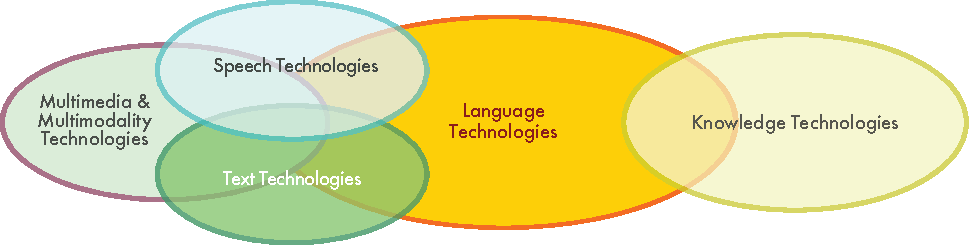
\includegraphics[width=\textwidth]{../_media/english/language_technologies}
  \caption{Language technologies}
  \label{fig:ltincontext_en}
  \colorrule{grey3}{\textwidth}{1.5pt}
\end{figure*}

When we communicate, we combine language with other modes of communication and information media -- for example speaking can involve gestures and facial expressions. Digital texts link to pictures and sounds. Movies may contain language in spoken and written form. In other words, speech and text technologies overlap and interact with other multimodal communication and multimedia technologies.

In this section, we will discuss the main application areas of language technology, i.\,e., language checking, web search, speech interaction, and machine translation. These applications and basic technologies include 

\begin{itemize}
\item spelling correction
\item authoring support
\item computer-assisted language learning
\item information retrieval 
\item information extraction
\item text summarisation
\item question answering
\item speech recognition 
\item speech synthesis 
\end{itemize}

\begin{figure*}[b]
  \colorrule{grey3}{\textwidth}{1.5pt}
  \center
  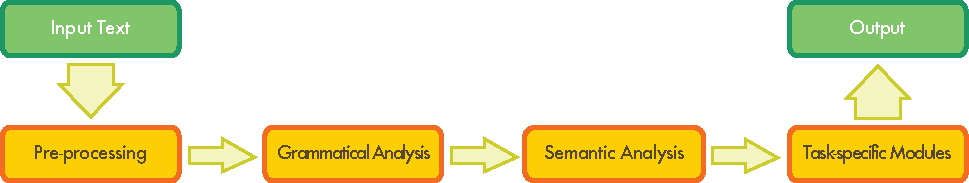
\includegraphics[width=\textwidth]{../_media/english/text_processing_app_architecture}
  \caption{A typical text processing architecture}
  \label{fig:textprocessingarch_en}
  \colorrule{grey3}{\textwidth}{1.5pt}
\end{figure*}

Language technology is an established area of research with an extensive set of introductory literature. The interested reader is referred to the following references: \cite{jurafsky-martin01,manning-schuetze1,lt-world1,lt-survey1}.

Before discussing the above application areas, we will briefly describe the architecture of a typical LT system.

\subsection{Application Architectures}

Software applications for language processing typically consist of several components that mirror different aspects of language. While such applications tend to be very complex, figure~\ref{fig:textprocessingarch_en} shows a highly simplified architecture of a typical text processing system. The first three modules handle the structure and meaning of the text input:

\begin{enumerate}
\item Pre-processing: cleans the data, analyses or removes formatting, detects the input languages, and so on.
\item Grammatical analysis: finds the verb, its objects, modifiers and other sentence elements; detects the sentence structure.
\item Semantic analysis: performs disambiguation (i.\,e., computes the appropriate meaning of words in a given context); resolves anaphora (i.\,e., which pronouns refer to which nouns in the sentence); represents the meaning of the sentence in a machine-readable way.
\end{enumerate}

After analysing the text, task-specific modules can perform other operations, such as automatic summarisation and database look-ups.

In the remainder of this section, we firstly introduce the core application areas for language technology, and follow this with a brief overview of the state of LT research and education today, and a description of past and present research programmes. Finally, we present an expert estimate of core LT tools and resources for spanish in terms of various dimensions such as availability, maturity and quality. The general situation of LT for the spanish language is is summarised in figure~\ref{fig:lrlttable_en} (p.~\pageref{fig:lrlttable_en}) at the end of this chapter. This table lists all tools and resources that are boldfaced in the text. LT support for spanish is also compared to other languages that are part of this series.

\subsection{Core Application Areas}

In this section, we focus on the most important LT tools and resources, and provide an overview of LT activities in Spain.

\subsubsection{Language Checking}

\begin{figure*}[t]
  \colorrule{grey3}{\textwidth}{1.5pt}
  \center
  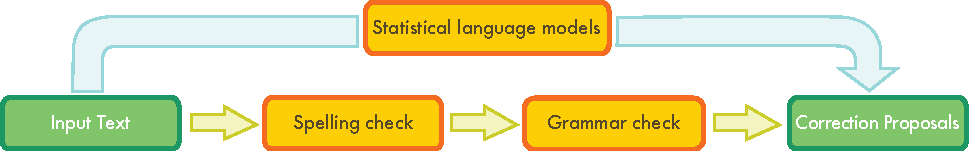
\includegraphics[width=\textwidth]{../_media/english/language_checking}
  \caption{Language checking (top: statistical; bottom: rule-based)}
  \label{fig:langcheckingaarch_en}
  \colorrule{grey3}{\textwidth}{1.5pt}
\end{figure*}

Anyone who has used a word processor such as Microsoft Word knows that it has a spelling checker that highlights spelling mistakes and proposes corrections. The first spelling correction programs compared a list of extracted words against a dictionary of correctly spelled words. Today these programs are far more sophisticated. Using language-dependent algorithms for \textbf{text analysis}, they detect errors related to morphology (e.g., plural formation) as well as syntax--related errors, such as a missing verb or a conflict of verb-subject agreement (e.g., she *write a letter). But most spell checkers will not find any errors in the following text:

\begin{quote}
  Eye have a spelling chequer,\\
  It came with my Pea Sea.\\
  It plane lee marks four my revue\\
  Miss Steaks I can knot sea.\cite{zar1}
\end{quote}

Handling these kinds of errors usually requires an analysis of the context. For Spanish, even spell checking requires analyzing the context in many cases. A typical case is when the orthographic error transforms one word into another, which also exits. In the following example, the first sentence contains a couple of frequent errors (problems with orthographic accents and omission of silent /h/). The second sentence is the corrected version of the first:

\begin{itemize}
  \item[] Mí calculo es que hoy a venido mas publico que ayer.
  \item[] [Me I-estimate that today to come but I-publish than yester-day]
  \item[] Mi cálculo es que hoy ha venido más público que ayer.
  \item[] [My estimation is that today has come more people (audience) than yesterday]
\end{itemize}

This type of analysis either needs to draw on language-specific \textbf{grammars} laboriously coded into the software by experts, or on a statistical language model. In this case, a model calculates the probability of a particular word as it occurs in a specific position (e.g., between the words that precede and follow it). For example, \textit{Mi cálculo or ha venido} are far much probable word sequences than \textit{Mí calculo or a venido} respectively. A statistical language model can be automatically created by using a large amount of (correct) language data (called a \textbf{text corpus}). Most of these two approaches have been developed around data from English. However, they do not necessarily transfer well to other languages, e.\,g.highly inflectional ones or languages with a flexible word order like Spanish. For these more complex languages, an advanced high-precision language checker may require the development of more sophisticated methods, involving a deeper linguistic analysis. 
\columnbreak

\boxtext{The use of language checking is not limited to word processors; it also applies to authoring support systems.}

Language checking is not limited to word processors; it is also used in “authoring support systems”, i.e., software environments in which manuals and other documentation are written to special standards for complex IT, healthcare, engineering and other products. Fearing customer complaints about incorrect use and damage claims resulting from poorly understood instructions, companies are increasingly focusing on the quality of technical documentation while targeting the international market (via translation or localization) at the same time. Advances in natural language processing have led to the development of authoring support software, which helps the writer of technical documentation use vocabulary and sentence structures that are consistent with industry rules and (corporate) terminology restrictions.

Only a few Spanish companies offer products in this area. For example Daedalus, born as a spin-off of two research groups from the Universidad Politécnica de Madrid (UPM) and the Universidad Autónoma de Madrid (UAM), has developed STILUS, a spelling, grammar and stylistic proof-reader for texts in Spanish. The technology is freely available through their web portal, but it can also be integrated in any content management tool. WinCorrect is a speller and grammar checker developed by Maxigramar (also with a free online version) and Signum is a Ecuador based SME that developed the spellchecker for Spanish licensed by Microsoft for their Office suite.

Besides spell checkers and authoring support, language checking is also important in the field of computer-assisted language learning. And language checking applications also automatically correct search engine queries, as found in Google's \textit{Did you mean\ldots} suggestions.

\subsubsection{Web Search}

\begin{figure*}[htb]
  \colorrule{grey3}{\textwidth}{1.5pt}
  \center
  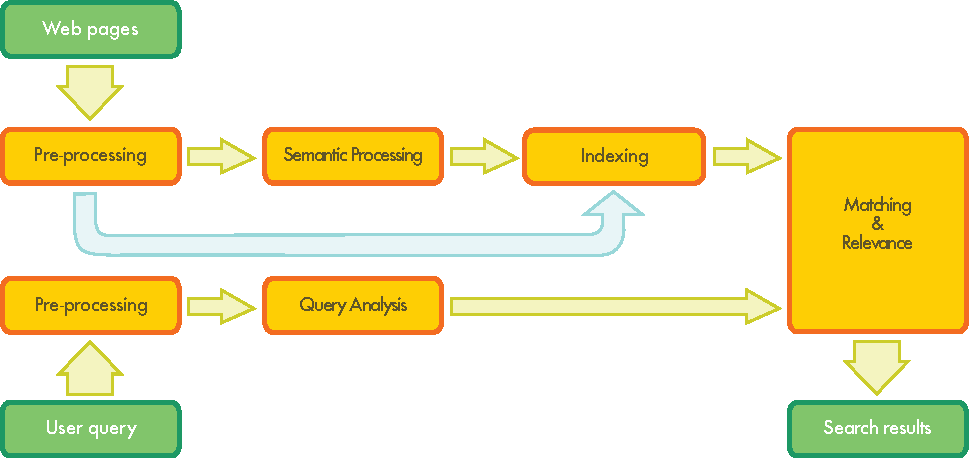
\includegraphics[width=\textwidth]{../_media/english/web_search_architecture}
  \caption{Web search}
  \label{fig:websearcharch_en}
  \colorrule{grey3}{\textwidth}{1.5pt}
 \end{figure*}

Searching the Web, intranets or digital libraries is probably the most widely used yet largely underdeveloped language technology application today. The Google search engine, which started in 1998, now handles about 80\% of all search queries. The Google search interface and results page display has not significantly changed since the first version. Yet in the current version, Google offers spelling correction for misspelled words and has recently incorporated basic semantic search capabilities that can improve search accuracy by analysing the meaning of terms in a search query context.  The Google success story shows that a large volume of available data and efficient indexing techniques can deliver satisfactory results for a statistically-based approach.

For more sophisticated information requests, it is essential to integrate deeper linguistic knowledge for \textbf{text interpretation}. Experiments using \textbf{lexical resources} such as machine-readable thesauri or ontological language resources (e.\,g.WordNet) have demonstrated improvements in finding pages using synonyms of the original search terms, such as e.\,g. „Energía atómica” and „Energía nuclear”, or even more loosely related terms. 

\boxtext{The next generation of search engines will have to include much more sophisticated language technology.}

The next generation of search engines will have to include much more sophisticated language technology, in particular in order to deal with search queries consisting of a question or other sentence type rather than a list of keywords. For the query, „Give me a list of all companies that were taken over by other companies in the last five years,” the LT system needs to analyse the sentence syntactically and semantically as well as provide an index to quickly re-trieve relevant documents. A satisfactory answer will require syntactic parsing to analyse the grammatical structure of the sentence and determine that the user wants companies that have been acquired, not companies that acquired other companies. For the expression last five years, the system needs to determine the relevant years. And, the query needs to be matched against a huge amount of unstructured data to find the piece or pieces of relevant information the user wants. This is called „information retrieval”, and involves searching and ranking relevant documents. To generate a list of companies, the system also needs to recognize a particular string of words in a document as a company name, a process called „named entity recognition”.

A more demanding challenge is matching a query in one language with documents in another language. Cross-lingual information retrieval involves automatically translating the query into all possible target languages and then translating the results back into the source language. 

Now that data is increasingly found in non-textual formats, there is a need for services that deliver multimedia information retrieval by searching images, audio files and video data. In the case of audio and video files, a speech recognition module must convert the speech content into text (or into a phonetic representation) that can then be matched against a user query.

In Spain, a few SMEs develop linguistic technology aimed at multilingual search and information retrieval, both from the Internet and from internal information systems. Among the main ones, we find the following: iSOCO, Daedalus, Inbenta, Bitext  and Thera, the latter also as spin-off, in this case from the Universitat de Barcelona. Their technology incorporates tools of automatic translation, as well as components of named entity recognition, fuzzy search and semantic tagging.

These companies focus their development on providing add-ons and advanced search engines for special interest portals by using topic-relevant semantics. Due to the constant high demand for processing power, such search engines are only cost-effective when handling relatively small text corpora. The processing time is several thousand times higher than that needed by a standard statistical search engine like Google. These search engines are in high demand for topic-specific domain modelling, but they cannot be used on the Web with its billions and billions of documents.

\subsubsection{Speech Interaction}

Speech interaction technology is used to create interfaces that enable users to interact in spoken language instead of a graphical display, keyboard and mouse. Today, voice user interfaces (VUI) are usually used for partially or fully automated telephone services provided by companies to customers, employees or partners. Business domains that rely heavily on VUIs include banking, supply chain, public transportation, and telecommunications. Other uses of speech technology include interfaces to car navigation systems and the use of spoken language as an alternative to the graphical or touch-screen interfaces in smartphones. 

\begin{figure*}[htb]
  \colorrule{grey3}{\textwidth}{1.5pt}
  \center
  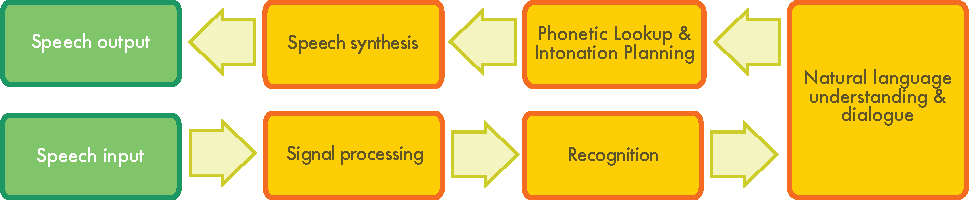
\includegraphics[width=\textwidth]{../_media/english/simple_speech-based_dialogue_architecture}
  \caption{Speech-based dialogue system}
  \label{fig:dialoguearch_en}
  \colorrule{grey3}{\textwidth}{1.5pt}
\end{figure*}

\boxtext{Speech interaction technology is the basis for creating interfaces that allow a user to interact with spoken language instead of a graphical display, keyboard and mouse.}

Speech interaction comprises four technologies:
\begin{enumerate}
  \item Automatic \textbf{speech recognition} (ASR) determines which words are actually spoken in a given sequence of sounds uttered by a user.  
  \columnbreak
  \item Natural language understanding analyses the syntactic structure of a user’s utterance and interprets it according to the system in question.
  \item Dialogue management determines which action to take given the user input and system functionality.   
  \item \textbf{Speech synthesis} (text-to-speech or TTS) transforms the system’s reply into sounds for the user.
\end{enumerate}

One of the major challenges of ASR systems is to accurately recognise the words a user utters. This means restricting the range of possible user utterances to a limited set of keywords, or manually creating language models that cover a large range of natural language utterances. Using machine learning techniques, language models can also be generated automatically from \textbf{speech corpora}, i.e., large collections of speech audio files and text transcriptions. Restricting utterances usually forces people to use the voice user interface in a rigid way and can damage user acceptance; but the creation, tuning and maintenance of rich language models will significantly increase costs. VUIs that employ language models and initially allow a user to express their intent more flexibly -- prompted by a \textit{How may I help you?} greeting -- tend to be automated and are better accepted by users. 

Companies tend to use pre-recorded utterances by professional speakers for generating the output of the voice user interface. For static utterances where the wording does not depend on particular contexts of use or personal user data, this can deliver a rich user experience. But more dynamic content in an utterance may suffer from unnatural intonation because bits of audio files have simply been strung together. Today’s TTS systems are getting better (though they can still be optimized) at producing natural-sounding dynamic utterances.  

Interfaces in the market for speech interaction technology have been considerably standardised during the last decade in terms of their various technology components. There has also been strong market consolidation in speech recognition and speech synthesis. The national markets in the G20 countries (economically resilient countries with high populations) have been dominated by just five global players, with Nuance (USA) and Loquendo (Italy) being the most prominent players in Europe , also for Spanish, although some smaller local companies are starting to compete, such as Verbio , which is a spin-off of Universitat Politècnica de Catalunya and has its own speech technology. 

Regarding dialogue management technology and know-how, markets are strongly dominated by national players, which are usually SMEs.

Most of the companies on the Spanish TTS market are essentially application developers. Key players in the Spanish market are: Indsys  (Intelligent Dialogue Systems), Fonetic , Ydilo  and NaturalVoz . Rather than relying on a software license-driven product business, these companies are mainly positioned as full-service providers that create voice user interfaces as part of a system integration service. In the area of speech interaction, there is as yet no real market for syntactic and semantic analysis-based core tech-nologies.

The demand for voice user interfaces in Spain has grown fast in the last five years, driven by increasing demand for customer self-service, cost optimisation for automated telephone services, and the increasing acceptance of spoken language as a media for human-machine interaction. 

Looking forward, there will be significant changes due to the spread of smartphones as a new platform for managing customer relationships in addition to fixed telephones, the Internet and e-mail. This will also affect how speech interaction technology is used. In the long run, there will be fewer telephone-based VUIs and spoken language will play a far more central role as a user-friendly input for smartphones. This will be largely driven by stepped im-provements in the accuracy of speaker-independent speech recognition via speech dictation services already offered as centralised services to smartphone users.

\subsubsection{Machine Translation}

The idea of using digital computers to translate natural languages can be traced back to 1946 and was followed by substantial funding for research during the 1950s and again in the 1980s. Yet \textbf{machine translation} (MT) still cannot deliver on its initial promise of providing across-the-board automated translation.

\boxtext{At its basic level, machine translation simply substitutes words in one natural language with words in another language.}

The most basic approach to machine translation is to automatically replace the words in a text in one natural language by words in another language. This can be useful in subject domains that have a very restricted, formulaic language such as weather reports. But to produce a good translation of less standardized texts, larger text units (phrases, sentences, or even whole passages) need to be matched to their closest counterparts in the target language. The major difficulty is that human language is ambiguous. Ambiguity creates challenges on multiple levels, such as word sense disambiguation on the lexical level (a \textit{jaguar} is a brand of car or an animal) or the assignment of case on the syntactic level, for example:

\begin{itemize}
  \item[] The woman saw the car and her husband, too.
  \item[] [La mujer vio el coche y su marido también.]
  \item[] [La mujer vio el coche y a su marido también..]
\end{itemize}

One way to build an MT system is to use linguistic rules. For translations between closely related languages, a direct substitution translation may be feasible in cases like the above example. But, rule-based (or linguistic knowledge-driven) systems often analyse the input text and create an intermediary symbolic representation from which the text can be generated into the target language. The success of these methods is highly dependent on the availability of extensive lexicons with morphological, syntactic, and semantic information, and large sets of grammar rules carefully designed by skilled linguists. This is a very long and therefore costly process.

\begin{figure*}[htb]
  \colorrule{grey3}{\textwidth}{1.5pt}
  \center
  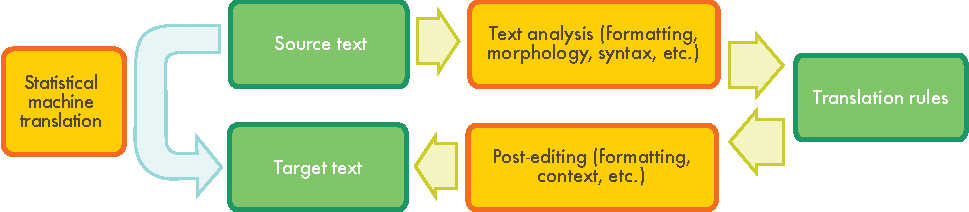
\includegraphics[width=\textwidth]{../_media/english/machine_translation}
  \caption{Machine translation (left: statistical; right: rule-based)}
  \label{fig:mtarch_en}
  \colorrule{grey3}{\textwidth}{1.5pt}
\end{figure*}
 
In the late 1980s when computational power increased and became cheaper, there was more interest in statistical models for machine translation. Statistical models are derived from analysing bilingual text corpora, such as the Europarl \textbf{parallel} corpus, which contains the proceedings of the European Parliament in 11 European languages. Given enough data, statistical MT works well enough to derive an approximate meaning of a foreign language text by pro-cessing parallel versions and finding plausible patterns of words. But unlike knowledge-driven systems, statistical (or data-driven) MT often generates ungrammatical output. Data-driven MT is advantageous because less human effort is required, and it can also cover special particularities of the language (e.g., idiomatic expressions) that can get ignored in knowledge-driven systems.

The strengths and weaknesses of knowledge-driven and data-driven machine translation tend to be complementary, so that nowadays researchers focus on hybrid approaches that combine both methodologies. One approach uses both knowledge-driven and data-driven systems together with a selection module that decides on the best output for each sentence. However, results for sentences longer than say 12 words will often be far from perfect. A better solution is to combine the best parts of each sentence from multiple outputs; this can be fairly complex, as corresponding parts of multiple alternatives are not always obvious and need to be aligned. 

Leading international MT developer Lucy Software has an important subsidiary in Spain, Lucy Iberica , former Translendium. Lucy Iberica is responsible for the development of language pairs that include Spanish and all language pairs involving any other Iberian language (Catalan, Portuguese, Galician and Basque). Word Magic is a popular Spanish-English (and viceversa) system developed by a US-based company. Both Lucy and Word Magic systems are grammar rule-based. While there is significant research in data-driven and hybrid systems in national and interna-tional contexts, this technology has been less successful in business than in research so far, with just a few companies offering statistical MT customization, such as Pangeanic. 

Apertium is a free open-source machine translation platform that provides a language-independent machine translation engine initially designed by the Transducens group at the Universitat d'Alacant and subsequently developed in the framework of  the nationally funded Opentrad project. Among current MT systems using Apertium technology, we find interNOSTRUM (Spanish-Catalan), Traductor Universia (Spanish-Portuguese) and Matxin (Basque-Spanish), the former developed by Transducens and the latter by the IXA group  at Euskal Herriko Unibertsitatea. It is possible to use Apertium to build machine translation systems for a variety of language pairs (there are over 20 to date); to that end, Apertium uses simple XML-based standard formats to encode the linguistic data needed (either by hand or by converting existing data), which are compiled using the provided tools into the high-speed formats used by the engine.

\boxtext{The use of machine translation can significantly increase productivity provided the system is adapted to user-specific terminology and inte-grated into a workflow. }

The use of machine translation can significantly increase productivity provided the system is intelligently adapted to user-specific terminology and integrated into a workflow. 

There is still a huge potential for improving the quality of MT systems. The challenges involve adapting language resources to a given subject domain or user area, and integrating the technology into workflows that already have term bases and translation memories.

Another problem is that most of the current systems are English-centred and only support a few languages from and into Spanish. This leads to friction in the translation workflow and forces MT users to learn different lexicon coding tools for different systems.

Evaluation campaigns help compare the quality of MT systems, the different approaches and the status of the systems for different language pairs. Figure~\ref{fig:euromatrix_es} (p.~\pageref{fig:euromatrix_es}), which was prepared during the EC Euromatrix+ project, shows the pair-wise performances obtained for 22 of the 23 official EU languages. (Irish Gaelic was not compared.) The results are ranked according to a BLEU score, which indicates higher scores for better translations.\cite{bleu1} (A human translator would achieve a score of around 80 points.) 

The best results (in green and blue) were achieved by languages that benefit from a considerable research effort in coordinated programs and from the existence of many parallel corpora (e.g., English, French, Dutch, Spanish and German). The languages with poorer results are shown in red. These languages either lack such development efforts or are structurally very different from other languages (e.g., Hungarian, Maltese and Finnish).

\subsection{Other Application Areas}

\boxtext{Language technology applications often provide significant service functionalities “under the hood” of larger software systems.}

Building language technology applications involves a range of subtasks that do not always surface at the level of interaction with the user, but they provide significant service functionalities “under the hood” of the system in question. They all form important research issues that have now evolved into individual sub-disciplines of computational linguistics. 

Question answering, for example, is an active area of research for which annotated corpora have been built and scientific competitions have been initiated. The concept of question answering goes beyond keyword-based searches (in which the search engine responds by delivering a collection of potentially relevant documents) and enables users to ask a concrete question to which the system provides a single answer. For example:

\begin{itemize}
\item[] \textit{Question: How old was Neil Armstrong when he stepped on the moon?}
\item[] \textit{Answer: 38.}
\end{itemize}

While question answering is obviously related to the core area of web search, it is nowadays an umbrella term for such research issues as what different types of questions there are, and how they should be handled; how a set of documents that potentially contain the answer can be analysed and compared (do they provide conflicting answers?); and how specific information (the answer) can be reliably extracted from a document without ignoring the context. 

This is in turn related to information extraction (IE), an area that was extremely popular and influential when computational linguistics took a statistical turn in the early 1990s. IE aims to identify specific pieces of information in specific classes of documents, such as detecting the key players in company takeovers as reported in newspaper stories. Another common scenario that has been studied is reports on terrorist incidents. The problem here is to map the text to a template that specifies the perpetrator, target, time, location and results of the incident. Domain-specific template-filling is the central characteristic of IE, which makes it another example of a “behind the scenes” technology that forms a well-demarcated research area that in practice needs to be embedded into a suitable application environment. 

Text summarization and \textbf{text generation} are two borderline areas that can act either as standalone applications or play a supporting role “under the hood”. Summarization attempts to give the essentials of a long text in a short form, and is one of the features available in Microsoft Word. It mostly uses a statistical approach to identify the “important” words in a text (i.e., words that occur very frequently in the text in question but less frequently in general language use) and determine which sentences contain the most of these “important” words. These sentences are then extracted and put together to create the summary. In this very common commercial scenario, summarization is simply a form of sentence extraction, and the text is reduced to a subset of its sentences. An alternative approach, for which some research has been carried out, is to generate brand new sentences that do not exist in the source text. This requires a deeper understanding of the text, which means that so far this approach is far less robust. On the whole, a text generator is rarely used as a stand-alone application but is embedded into a larger software environment, such as a clinical information system that collects, stores and processes patient data. Creating reports is just one of many applications for text summarization.

\boxtext{For the Spanish language, research in most text technologies is much less developed than for the English language.}

For the Spanish language, research in these text technologies is much less developed than for the English language. Question answering, information extraction, and summarization have been the focus of numerous open competitions in the USA since the 1990s, primarily organised by the government-sponsored organisations DARPA and NIST. These competitions have significantly improved the start-of-the-art, but their focus has mostly been on the English language. As a result, there are hardly any annotated corpora or other special resources needed to perform these tasks in Spanish. When summarization systems use purely statistical methods, they are largely language-independent and a number of research prototypes are available. For text generation, reusable components have traditionally been limited to surface realization modules (generation grammars) and most of the available software is for the English language.

Apart from the experimental systems being developed by the research groups, there are a few SMEs offering this kind of services. Among them Daedalus and Inbenta, and some international companies with a significant presence in the Spanish market, such as Q-go  and Artificial Solutions.

\subsection{Educational Programmes}

Language Technology is a highly interdisciplinary field, involving the expertise of linguists, computer scientists, mathematicians, philosophers, psycholinguists, and neuroscientists, among others. Consequently, the current basic training of a computational linguist may be performed in Spain within the framework of a degree in Philology or Linguistics, which includes Computational Linguistics as a core subject, or by Computational Science faculties. Among the Universities that offer the first option: Universitat de Barcelona, Universitat Pompeu Fabra, Universitat Oberta de Catalunya and Universidade de Vigo. On the other hand, main computational science faculties offering Computational Linguistic as subject are: Universidad Politécnica de Madrid, Universidad Carlos III, Universidad Autónoma de Madrid, Universitat d’Alacant, Universidad Nacional de Educación a Distancia, and Euskal Herriko Unibertsitatea. Other cases, such as the Universidad Complutense combine both.

Graduate courses offer a more targeted professional training. There are several doctoral programs which offer masters or subjects related to language and speech processing. Certain universities such as the Universitat Politècnica de Catalunya also participate in the European Masters in Language and Speech sponsored by ELSNET (European Network of Excellence in Human Language Technologies). Masters are often offered by a group of universities, either at state or at European level. For example, the Universitat Autònoma de Barcelona offers the International Master in Natural Language Processing and Human Language Technology, in collaboration with foreign universities. Modules in Language Technology are also offered to students of other master or PhD courses, particularly in Translation (e.\,g.Autònoma de Barcelona, Alacant, Castelló, Politècnica de València, Granada).

\boxtext{There are over 30 research groups in Spain spread across the universities, working on speech recognition, natural language processing, text-to-text translation and speech synthesis.}

There are over 30 research groups in Spain spread across the universities, working on speech recognition, natural language processing, text-to-text translation and speech synthesis. The Sociedad Española para el Procesamiento del Lenguaje Natural (SEPLN, Spanish Society for Natural Language Processing), is a non-profit organization with over 300 members, both from academia and industry, which was created in 1984 with the purpose to promote and spread activities related to teaching, research and development of NLP, on both national and international level. SEPLN organizes seminaries, symposiums and conferences and promotes collaboration with national and international institutions.

SEPLN organizes an annual conference, which is attended yearly by an increasing number of researchers working on NLP, both from Spain and abroad. The association also edits a periodical journal and maintains a web server with information about issues related to the natural language processing and an open forum for members. 

\subsection[National Projects and Initiatives]{National Projects\newline and Initiatives}

The Ministry of Education, through the Interministerial Commission of Science and Technology (CICYT), which is the body that coordinates and monitors national strategy plans for Science \& Technology in Spain, has supported research in the field of information technologies through national research programs. These programs have impelled numerous research projects and collaboration with international research centers and companies. The basis of technology development and commercial applications for automated processing of the Spanish language has been partly created as a result of these projects.

The Centre for the Development of Industrial Technology (CDTI) is a Spanish public organisation, under the Ministry of Science and Innovation, whose objective is to help Spanish companies to increase their technological profile. CDTI evaluates and finances R\&D projects through programmes such as CENIT, AVANZA and INNPACTO.

The CENIT (National Strategic Consortiums for Technological Re-search) programme seeks to stimulate cooperation in R\&D between the private sector, universities, public research organisations and centres, science and technology parks and technological centres, boosting public and private-sector cooperation in R\&D. CENIT projects last at least four years and have a minimum budget of €5 mill. a year during which they will receive minimum funding of 50\% from the private sector. At least 50\% of public funding will be allocated to public research centres or technological centres. Information Technology and Communication is one of the programme’s priority areas. Projects in this area sometimes include research in Language Technologies. 

The aim of the AVANZ@ and INNPACTO Plans are to bring the Information Society to ordinary citizens, and to private and public sectors. Promoting the use of ICT technologies will have a knock-on effect on the whole sector in Spain, therefore on its innovation status. The Plan’s objectives include increasing the percentage of businesses using e-commerce; promoting the use of electronic billing; extending the electronic public sector by implementing an electronic identity card and electronic registration; attaining a rate of one Internet-connected computer for every two students in schools; and doubling the number of homes with Internet access. Among their priorities is to facilitate the use of new technologies to old people and people with disabilities, as an ideal means to achieve social integration, avoid exclusion and improve their quality of life. User-friendly language technology tools offer the principal solution to satisfy this goal, for example by offering speech synthesis for the blind.

Previous projects and programmes have led to the development of a number of LT tools and resources for the Spanish language. In the following section, the current state of LT support for Spanish is summarized.  

\subsection{Availability of Tools and Resources}

The following table summarizes the current state of language technology support for the Spanish language. The rating for existing tools and resources is based on educated estimates of leading experts.

\begin{figure*}[htb]
\centering
%\begin{tabular}{>{\columncolor{orange1}}p{.33\linewidth}ccccccc} % ORIGINAL
\begin{tabular}{>{\columncolor{orange1}}p{.33\linewidth}@{\hspace*{6mm}}c@{\hspace*{6mm}}c@{\hspace*{6mm}}c@{\hspace*{6mm}}c@{\hspace*{6mm}}c@{\hspace*{6mm}}c@{\hspace*{6mm}}c}
\rowcolor{orange1}
 \cellcolor{white}&\begin{sideways}\makecell[l]{Quantity}\end{sideways}
&\begin{sideways}\makecell[l]{\makecell[l]{Availability} }\end{sideways} &\begin{sideways}\makecell[l]{Quality}\end{sideways}
&\begin{sideways}\makecell[l]{Coverage}\end{sideways} &\begin{sideways}\makecell[l]{Maturity}\end{sideways} &\begin{sideways}\makecell[l]{Sustainability~~~}\end{sideways} &\begin{sideways}\makecell[l]{Adaptability}\end{sideways} \\ \addlinespace
\multicolumn{8}{>{\columncolor{orange2}}l}{Language Technology: Tools, Technologies and Applications} \\ \addlinespace
Speech Recognition	&4&2&3.6&4.8&4&4&3 \\ \addlinespace
Speech Synthesis &4&2&4.8&4.8&4&4&3\\ \addlinespace
Grammatical analysis &3.5&3&5.4&4.5&3.5&3&3.5\\ \addlinespace
Semantic analysis &1.5&2&2.4&2.4&2&2&1\\ \addlinespace
Text generation &1&2&2.4&2.4&2&1&2\\ \addlinespace
Machine translation &5&4&6&4.8&5&3&3\\ \addlinespace
\multicolumn{8}{>{\columncolor{orange2}}l}{Language Resources: Resources, Data and Knowledge Bases} \\ \addlinespace
Text corpora &3&2.5&3.6&3.6&3&3.5&3.5\\ \addlinespace
Speech corpora &3&1&3.6&2.4&3&4&3\\ \addlinespace
Parallel corpora &4&3&4.8&3.6&3&2&2\\ \addlinespace
Lexical resources &3&3&3.6&3.6&3.5&3.5&2.5\\ \addlinespace
Grammars &2&3&3.6&3.6&4&2&3\\
\end{tabular}
\caption{State of language technology support for spanish}
\label{fig:lrlttable_en}
\end{figure*}

The key results for the Spanish language can be summed up as follows:

\begin{itemize}
\item	Speech processing currently seems to be slightly more mature than the processing of written text. In fact, speech technology has already been successfully integrated into many everyday applications, from spoken dialogue systems and voice-based interfaces to mobile phones and car navigation systems.
\item	Research has successfully led to the design of medium to high quality software for basic text analysis, such as tools for morphological analysis and syntactic parsing. But advanced technologies that require deep linguistic processing and semantic knowledge are still in their infancy.
\item	As to resources, there is a large reference text corpus with a balanced mix of genres for the Spanish language, but it is not easily available for research. There are a number of corpora annotated with syntactic, semantic and discourse structure mark-up, but again, there are not nearly enough language corpora containing the right sort of content to meet the growing need for more deep linguistic and semantic information.
\item	In particular, there is a lack of the sort of parallel corpora that form the basis for statistical and hybrid approaches to machine translation. Parallel corpora exist, between Spanish and English, and between Spanish and other languages from Spain. However, parallel corpora between Spanish and other languages are mostly missing.
\item	Many of these tools, resources and data formats do not meet industry standards and cannot be sustained effectively. A concerted programme is required to standardise data formats and APIs.
\item	An unclear legal situation restricts making use of digital texts, such as those published online by newspapers, for empirical linguistic and language technology research, for example, to train statistical language models. Together with politicians and policy makers, researchers should try to establish laws or regulations that enable them to use publicly available texts for language-related R\&D activities.
\item	The cooperation between the Language Technology community and those involved with the Semantic Web and the closely related Linked Open Data movement should be intensified with the goal of establishing a collaboratively maintained, machine-readable knowledge base that can be used both in web-based in-formation systems and as semantic knowledge bases in LT applications -- ideally, this endeavour should be addressed in a multilingual way on the European scale. 
\end{itemize}

To conclude, in a number of specific areas of Spanish language research, we have software with limited functionality available today. Obviously, further research efforts are required to meet the current deficit in processing texts on a deeper semantic level and to address the lack of resources such as parallel corpora for machine translation.

\subsection{Cross-language comparison}

The current state of LT support varies considerably from one language community to another. In order to compare the situation between languages, this section will present an evaluation based on two sample application areas (machine translation and speech processing) and one underlying technology (text analysis), as well as basic resources needed for building LT applications. The languages were categorised using the following five-point scale: 

\begin{enumerate}
\item Excellent support
\item Good support
\item Moderate support
\item Fragmentary support
\item Weak or no support
\end{enumerate}

LT support was measured according to the following criteria:

\textbf{Speech Processing:} Quality of existing speech recognition technologies, quality of existing speech synthesis technologies, coverage of domains, number and size of existing speech corpora, amount and variety of available speech-based applications.

\textbf{Machine Translation:} Quality of existing MT technologies, number of language pairs covered, coverage of linguistic phenomena and domains, quality and size of existing parallel corpora, amount and variety of available MT applications.

\textbf{Text Analysis:} Quality and coverage of existing text analysis technologies (morphology, syntax, semantics), coverage of linguistic phenomena and domains, amount and variety of available applications, quality and size of existing (annotated) corpora, quality and coverage of lexical resources (e.\,g., WordNet) and grammars.

\textbf{Resources:} Quality and size of existing text corpora, speech corpora and parallel corpora, quality and coverage of existing lexical resources and grammars.

The tables~\ref{fig:speech_cluster_en} to~\ref{fig:resources_cluster_en} show that, thanks to large-scale LT funding in recent decades, the Spanish language is better equipped than most other languages. It compares well with most large languages, such as French and German. But LT resources and tools for Spanish clearly do not yet reach the quality and coverage of comparable resources and tools for the English language, which is in the lead in almost all LT areas. And there are still plenty of gaps in English language resources with regard to high quality applications.

For speech processing, current technologies perform well enough to be successfully integrated into a number of industrial applications such as spoken dialogue and dictation systems. Today’s text analysis components and language resources already cover most surface linguistic phenomena of Spanish and form part of many applications involving mostly shallow natural language processing, e.\,g.spelling correction and authoring support.

However, for building more sophisticated applications, such as machine translation, there is a clear need for resources and technologies that cover a wider range of linguistic aspects and allow a deep semantic analysis of the input text. By improving the quality and coverage of these basic resources and technologies, we shall be able to open up new opportunities for tackling a vast range of advanced application areas, including high-quality machine translation.

\subsection{Conclusions}

\emph{In this series of white papers, we have made an important initial effort to assess language technology support for 30 European languages, and provide a high-level comparison across these languages. By identifying the gaps, needs and deficits, the European language technology commu-nity and related stakeholders are now in a position to design a large scale research and development programme aimed at building a truly multilingual, technology-enabled Europe.}

We have seen that there are huge differences between Europe’s languages. While there are good quality software and resources available for some languages and application areas, others (usually ‘smaller’ languages) have substantial gaps. Many languages lack basic technologies for text analysis and the essential resources for developing these technologies. Others have basic tools and resources but are as yet unable to invest in semantic processing. We therefore still need to make a large-scale effort to attain the ambitious goal of providing high-quality machine translation between all European languages.  

We can be cautiously optimistic about technology support for the Spanish language. There is an LT industry and research scene in Spain, which was previously supported by large research programs, many of them in large industrial corporations. A number of large-scale resources and state-of-the-art technologies have been produced and distributed for Spanish. However, the size of the resources and the number of tools is still very limited when compared to the resources and tools for the English language, and they are simply not extensive enough to develop the technologies that are required to support a truly multilingual knowledge society.

Unfortunately, there is only a relatively small language technology industry at work on the Spanish language. Most large companies have stopped or severely decreased their LT work, leaving the field to a small population of specialized SMEs that are unable to address an international market in which the language barrier is a key factor holding back cross-border e-commerce in the EU \cite{EUecommerce}.

It is clear that there must be a greater effort to create LT resources for Spanish, and drive research, innovation and development in general. The need for large amounts data and the extreme complexity of language technology systems makes it vital to develop a new infrastructure to spur greater sharing and cooperation.

There is also a lack of continuity in research and development funding. Short-term coordinated programmes tend to alternate with periods of low or sparse funding. In addition, there is an overall lack of coordination with programmes in other EU countries and at the European Commission level.

A large coordinated effort focused on language technologies would help the Spanish language, together with other languages, and establish a genuine multilingual agenda for Europe and the world as a whole \cite{HuLaTec}. 

META-NET’s long-term goal is to introduce high-quality language technology for all languages in order to achieve political and economic unity through cultural diversity. The technology will help tear down existing barriers and build bridges between Europe’s languages. This requires all stakeholders - in politics, research, business, and society - to unite their efforts for the future.

\end{multicols}

\clearpage

\begin{figure*}[t]
  \small
  \centering
  \begin{tabular}
  { % defines color for each column.
  >{\columncolor{corange5}}p{.13\linewidth}@{\hspace{.040\linewidth}}
  >{\columncolor{corange4}}p{.13\linewidth}@{\hspace{.040\linewidth}}
  >{\columncolor{corange3}}p{.13\linewidth}@{\hspace{.040\linewidth}}
  >{\columncolor{corange2}}p{.13\linewidth}@{\hspace{.040\linewidth}}
  >{\columncolor{corange1}}p{.13\linewidth} 
  }
  \multicolumn{1}{>{\columncolor{white}}c@{\hspace{.040\linewidth}}}{\textbf{Excellent}} & 
  \multicolumn{1}{@{}>{\columncolor{white}}c@{\hspace{.040\linewidth}}}{\textbf{Good}} &
  \multicolumn{1}{@{}>{\columncolor{white}}c@{\hspace{.040\linewidth}}}{\textbf{Moderate}} &
  \multicolumn{1}{@{}>{\columncolor{white}}c@{\hspace{.040\linewidth}}}{\textbf{Fragmentary}} &
  \multicolumn{1}{@{}>{\columncolor{white}}c}{\textbf{Weak/no}} \\ 
  \multicolumn{1}{>{\columncolor{white}}c@{\hspace{.040\linewidth}}}{\textbf{support}} & 
  \multicolumn{1}{@{}>{\columncolor{white}}c@{\hspace{.040\linewidth}}}{\textbf{support}} &
  \multicolumn{1}{@{}>{\columncolor{white}}c@{\hspace{.040\linewidth}}}{\textbf{support}} &
  \multicolumn{1}{@{}>{\columncolor{white}}c@{\hspace{.040\linewidth}}}{\textbf{support}} &
  \multicolumn{1}{@{}>{\columncolor{white}}c}{\textbf{support}} \\ \addlinespace
  
& \vspace*{0.5mm}English
& \vspace*{0.5mm}
Czech \newline 
Dutch \newline 
Finnish \newline 
French \newline 
German \newline   
Italian \newline  
Portuguese \newline 
\textbf{Spanish} \newline
& \vspace*{0.5mm}Basque \newline 
Bulgarian \newline 
Catalan \newline 
Danish \newline 
Estonian \newline 
Galician\newline 
Greek \newline  
Hungarian  \newline
Irish \newline  
Norwegian \newline 
Polish \newline 
Serbian \newline 
Slovak \newline 
Slovene \newline 
Swedish \newline
& \vspace*{0.5mm}
Croatian \newline 
Icelandic \newline  
Latvian \newline 
Lithuanian \newline 
Maltese \newline 
Romanian\\
\end{tabular}
\caption{Speech processing: State of language technology support for 30 European languages}
\label{fig:speech_cluster_en}
\end{figure*}

\begin{figure*}[b]
  \small
  \centering
  \begin{tabular}
  { % defines color for each column.
  >{\columncolor{corange5}}p{.13\linewidth}@{\hspace{.040\linewidth}}
  >{\columncolor{corange4}}p{.13\linewidth}@{\hspace{.040\linewidth}}
  >{\columncolor{corange3}}p{.13\linewidth}@{\hspace{.040\linewidth}}
  >{\columncolor{corange2}}p{.13\linewidth}@{\hspace{.040\linewidth}}
  >{\columncolor{corange1}}p{.13\linewidth} 
  }
  \multicolumn{1}{>{\columncolor{white}}c@{\hspace{.040\linewidth}}}{\textbf{Excellent}} & 
  \multicolumn{1}{@{}>{\columncolor{white}}c@{\hspace{.040\linewidth}}}{\textbf{Good}} &
  \multicolumn{1}{@{}>{\columncolor{white}}c@{\hspace{.040\linewidth}}}{\textbf{Moderate}} &
  \multicolumn{1}{@{}>{\columncolor{white}}c@{\hspace{.040\linewidth}}}{\textbf{Fragmentary}} &
  \multicolumn{1}{@{}>{\columncolor{white}}c}{\textbf{Weak/no}} \\ 
  \multicolumn{1}{>{\columncolor{white}}c@{\hspace{.040\linewidth}}}{\textbf{support}} & 
  \multicolumn{1}{@{}>{\columncolor{white}}c@{\hspace{.040\linewidth}}}{\textbf{support}} &
  \multicolumn{1}{@{}>{\columncolor{white}}c@{\hspace{.040\linewidth}}}{\textbf{support}} &
  \multicolumn{1}{@{}>{\columncolor{white}}c@{\hspace{.040\linewidth}}}{\textbf{support}} &
  \multicolumn{1}{@{}>{\columncolor{white}}c}{\textbf{support}} \\ \addlinespace
  
& \vspace*{0.5mm} English 
& \vspace*{0.5mm} 
French \newline 
\textbf{Spanish}
& \vspace*{0.5mm}
Catalan \newline 
Dutch \newline 
German \newline 
Hungarian \newline
Italian \newline 
Polish \newline 
Romanian \newline 
& \vspace*{0.5mm}Basque \newline 
Bulgarian \newline 
Croatian \newline 
Czech \newline
Danish \newline 
Estonian \newline 
Finnish \newline 
Galician \newline 
Greek \newline 
Icelandic \newline 
Irish \newline 
Latvian \newline 
Lithuanian \newline 
Maltese \newline 
Norwegian \newline 
Portuguese \newline 
Serbian \newline 
Slovak \newline 
Slovene \newline 
Swedish \newline 
\end{tabular}
\caption{Machine translation: State of language technology support for 30 European languages}
\label{fig:mt_cluster_en}
\end{figure*}

\begin{figure*}[t]
  \small
  \centering
  \begin{tabular}
  { % defines color for each column.
  >{\columncolor{corange5}}p{.13\linewidth}@{\hspace{.040\linewidth}}
  >{\columncolor{corange4}}p{.13\linewidth}@{\hspace{.040\linewidth}}
  >{\columncolor{corange3}}p{.13\linewidth}@{\hspace{.040\linewidth}}
  >{\columncolor{corange2}}p{.13\linewidth}@{\hspace{.040\linewidth}}
  >{\columncolor{corange1}}p{.13\linewidth} 
  }
  \multicolumn{1}{>{\columncolor{white}}c@{\hspace{.040\linewidth}}}{\textbf{Excellent}} & 
  \multicolumn{1}{@{}>{\columncolor{white}}c@{\hspace{.040\linewidth}}}{\textbf{Good}} &
  \multicolumn{1}{@{}>{\columncolor{white}}c@{\hspace{.040\linewidth}}}{\textbf{Moderate}} &
  \multicolumn{1}{@{}>{\columncolor{white}}c@{\hspace{.040\linewidth}}}{\textbf{Fragmentary}} &
  \multicolumn{1}{@{}>{\columncolor{white}}c}{\textbf{Weak/no}} \\ 
  \multicolumn{1}{>{\columncolor{white}}c@{\hspace{.040\linewidth}}}{\textbf{support}} & 
  \multicolumn{1}{@{}>{\columncolor{white}}c@{\hspace{.040\linewidth}}}{\textbf{support}} &
  \multicolumn{1}{@{}>{\columncolor{white}}c@{\hspace{.040\linewidth}}}{\textbf{support}} &
  \multicolumn{1}{@{}>{\columncolor{white}}c@{\hspace{.040\linewidth}}}{\textbf{support}} &
  \multicolumn{1}{@{}>{\columncolor{white}}c}{\textbf{support}} \\ \addlinespace

& \vspace*{0.5mm}English
& \vspace*{0.5mm}
  Dutch \newline 
  French \newline 
  German \newline 
  Italian \newline 
  \textbf{Spanish}
& \vspace*{0.5mm}Basque \newline 
  Bulgarian \newline 
  Catalan \newline 
  Czech \newline 
  Danish \newline 
  Finnish \newline 
  Galician \newline 
  Greek \newline 
  Hungarian \newline 
  Norwegian \newline 
  Polish \newline 
  Portuguese \newline 
  Romanian \newline 
  Slovak \newline 
  Slovene \newline 
  Swedish \newline 
& \vspace*{0.5mm}
  Croatian \newline 
  Estonian \newline 
  Icelandic \newline 
  Irish \newline 
  Latvian \newline 
  Lithuanian \newline 
  Maltese \newline 
  Serbian \\
  \end{tabular}
\caption{Text analysis: State of language technology support for 30 European languages}
\label{fig:text_cluster_en}
\end{figure*}

\begin{figure*}[b]
  \small
  \centering
  \begin{tabular}
  { % defines color for each column.
  >{\columncolor{corange5}}p{.13\linewidth}@{\hspace{.040\linewidth}}
  >{\columncolor{corange4}}p{.13\linewidth}@{\hspace{.040\linewidth}}
  >{\columncolor{corange3}}p{.13\linewidth}@{\hspace{.040\linewidth}}
  >{\columncolor{corange2}}p{.13\linewidth}@{\hspace{.040\linewidth}}
  >{\columncolor{corange1}}p{.13\linewidth} 
  }
  \multicolumn{1}{>{\columncolor{white}}c@{\hspace{.040\linewidth}}}{\textbf{Excellent}} & 
  \multicolumn{1}{@{}>{\columncolor{white}}c@{\hspace{.040\linewidth}}}{\textbf{Good}} &
  \multicolumn{1}{@{}>{\columncolor{white}}c@{\hspace{.040\linewidth}}}{\textbf{Moderate}} &
  \multicolumn{1}{@{}>{\columncolor{white}}c@{\hspace{.040\linewidth}}}{\textbf{Fragmentary}} &
  \multicolumn{1}{@{}>{\columncolor{white}}c}{\textbf{Weak/no}} \\ 
  \multicolumn{1}{>{\columncolor{white}}c@{\hspace{.040\linewidth}}}{\textbf{support}} & 
  \multicolumn{1}{@{}>{\columncolor{white}}c@{\hspace{.040\linewidth}}}{\textbf{support}} &
  \multicolumn{1}{@{}>{\columncolor{white}}c@{\hspace{.040\linewidth}}}{\textbf{support}} &
  \multicolumn{1}{@{}>{\columncolor{white}}c@{\hspace{.040\linewidth}}}{\textbf{support}} &
  \multicolumn{1}{@{}>{\columncolor{white}}c}{\textbf{support}} \\ \addlinespace
    
& \vspace*{0.5mm}English
& \vspace*{0.5mm} 
    Czech \newline 
    Dutch \newline 
    French \newline 
    German \newline 
    Hungarian \newline
    Italian \newline
    Polish \newline
    \textbf{Spanish} \newline
    Swedish \newline 
& \vspace*{0.5mm} Basque\newline 
    Bulgarian\newline 
    Catalan \newline 
    Croatian \newline 
    Danish \newline 
    Estonian \newline 
    Finnish \newline 
    Galician \newline 
    Greek \newline 
    Norwegian \newline 
    Portuguese \newline 
    Romanian \newline 
    Serbian \newline 
    Slovak \newline 
    Slovene \newline
&  \vspace*{0.5mm}
    Icelandic \newline 
    Irish \newline 
    Latvian \newline 
    Lithuanian \newline 
    Maltese  \\
  \end{tabular}
  \caption{Speech and text resources: State of support for 30 European languages}  
  \label{fig:resources_cluster_en}
\end{figure*}

\clearpage

% --------------------------------------------------------------------------
\ssection[About META-NET]{About META-NET}

\begin{multicols}{2}
META-NET is a Network of Excellence funded by the European Commission. The network currently consists of 54 members from 33 European countries \cite{rehm2011}. META-NET fosters the Multilingual Europe Technology Alliance (META), a growing community of language technology professionals and organisations in Europe. META-NET fosters the technological foundations for a truly multilingual European information society that:

\begin{itemize}
\item makes communication and cooperation possible across languages;
\item provides equal access to information and knowledge in any language;
\item offers advanced and affordable networked information technology to European citizens.
\end{itemize}

The network supports a Europe that unites as a single digital market and information space. It stimulates and promotes multilingual technologies for all European languages. These technologies support automatic translation, content production, information processing and knowledge management for a wide variety of applications and subject domains. They also enable intuitive language-based interfaces to technology ranging from household electronics, machinery and vehicles to computers and robots.

Launched on 1 February 2010, META-NET has already conducted various activities in its three lines of action META-VISION, META-SHARE and META-RESEARCH.

\textbf{META-VISION} fosters a dynamic and influential stakeholder community that unites around a shared vision and a common strategic research agenda (SRA). The main focus of this activity is to build a coherent and cohesive LT community in Europe by bringing together representatives from highly fragmented and diverse groups of stakeholders. The present White Paper was prepared together with volumes for 29 other languages. The shared technology vision was developed in three sectorial Vision Groups. The META Technology Council was established in order to discuss and to prepare the SRA based on the vision in close interaction with the entire LT community. 

\textbf{META-SHARE} creates an open, distributed facility for exchanging and sharing resources. The peer-to-peer network of repositories will contain language data, tools and web services that are documented with high-quality metadata and organised in standardised categories. The resources can be readily accessed and uniformly searched. The available resources include free, open source materials as well as restricted, commercially available, fee-based items.

\textbf{META-RESEARCH} builds bridges to related technology fields. This activity seeks to leverage advances in other fields and to capitalise on innovative research that can benefit language technology. In particular, the action line focuses on conducting leading-edge research in machine translation, collecting data, preparing data sets and organising language resources for evaluation purposes; compiling inventories of tools and methods; and organising workshops and training events for members of the community.

\textbf{\centerline{office@meta-net.eu -- http://www.meta-net.eu}}
\end{multicols}

\cleardoublepage

\appendix
\addtocontents{toc}{\protect\bigskip}

\phantomsection\bsection[Referencias -- References]{Referencias --- References}

\bibliographystyle{unsrt}
\bibliography{spanish_references}
  
\cleardoublepage

\phantomsection\bsection[META-NET Miembros -- META-NET Members]{META-NET Miembros --- META-NET Members}
\label{metanetmembers}

\small
\begin{longtable}{@{}llp{113mm}@{}}
  Alemania & \textcolor{grey1}{Germany} & Language Technology Lab, DFKI: Hans Uszkoreit, Georg Rehm \\ \addlinespace
  & & Human Language Technology and Pattern Recognition, RWTH Aachen University: Hermann Ney \\ \addlinespace
  & & Dept.~of Computational Linguistics, Saarland University: Manfred Pinkal \\ \addlinespace 
  Austria & \textcolor{grey1}{Austria} & Zentrum für Translationswissenschaft, Univ. Wien: Gerhard Budin \\ \addlinespace 
  Bélgica & \textcolor{grey1}{Belgium} & Computational Linguistics and Psycholinguistics Research Centre, Univ. of Antwerp: Walter Daelemans \\ \addlinespace
  & & Centre for Proc.~Speech and Images, Univ. of Leuven: Dirk van Compernolle \\ \addlinespace
  Bulgaria & \textcolor{grey1}{Bulgaria} & Institute for Bulgarian Language, Bulgarian Academy of Sciences: Svetla Koeva \\ \addlinespace
  Chipre & \textcolor{grey1}{Cyprus} & Language Centre, School of Humanities: Jack Burston \\ \addlinespace
  Croacia & \textcolor{grey1}{Croatia} & Institute of Linguistics, Faculty of Humanities and Social Science, Univ. of Zagreb: Marko Tadić \\ \addlinespace
  Dinamarca &  \textcolor{grey1}{Denmark} & Centre for Language Technology, Univ. of Copenhagen: Bolette Sandford Pedersen, Bente Maegaard \\ \addlinespace
  Eslovaquia & \textcolor{grey1}{Slovakia} & Ludovit Stur Institute of Linguistics, Slovak Academy of Sciences: Radovan Garabik \\ \addlinespace 
  Eslovenia & \textcolor{grey1}{Slovenia} & Jozef Stefan Institute: Marko Grobelnik \\ \addlinespace 
  España & \textcolor{grey1}{Spain} & Barcelona Media: Toni Badia \\ \addlinespace 
  & & Institut Universitari de Lingüistica Aplicada, Univ. Pompeu Fabra: Núria Bel \\ \addlinespace 
  & & Aholab Signal Processing Laboratory, Univ. of the Basque Country: Inma Hernaez Rioja \\ \addlinespace 
  & & Center for Language and Speech Technologies and Applications, Technical Univ. of Catalonia: Asunción Moreno \\ \addlinespace 
  & & Dept. of Signal Processing and Communications, Univ. of Vigo: Carmen García Mateo \\ \addlinespace 
  Estonia & \textcolor{grey1}{Estonia} & Institute of Computer Science, Univ. of Tartu: Tiit Roosmaa \\ \addlinespace
  Finlandia & \textcolor{grey1}{Finland} & Computational Cognitive Systems Research Group, Aalto Univ.: Timo Honkela \\ \addlinespace
  & & Dept. of General Linguistics, Univ. of Helsinki: Kimmo Koskenniemi, Krister Linden \\ \addlinespace
  Francia & \textcolor{grey1}{France} & Centre National de la Recherche Scientifique, Laboratoire d'Informatique pour la Mécanique et les Sciences de l'Ingénieur: Joseph Mariani \\ \addlinespace
  & & Evaluations and Language Resources Distribution Agency: Khalid Choukri \\ \addlinespace 
  Grecia & \textcolor{grey1}{Greece} & Institute for Language and Speech Processing, R.C. “Athena”: Stelios Piperidis \\ \addlinespace
  Holanda & \textcolor{grey1}{Netherlands} & Utrecht Institute of Linguistics, Utrecht Univ.: Jan Odijk \\ \addlinespace 
  & & Computational Linguistics, Univ. of Groningen: Gertjan van Noord \\ \addlinespace
  Hungría & \textcolor{grey1}{Hungary} & Research Inst. for Linguistics, Hungarian Academy of Sciences: Tamás Váradi \\  \addlinespace
  & & Dept. of Telecommunications and Media Informatics, Budapest Univ. of Technology and Economics: Géza Németh and Gábor Olaszy \\ \addlinespace
  Irlanda & \textcolor{grey1}{Ireland} & School of Computing, Dublin City Univ.: Josef van Genabith \\ \addlinespace
  Islandia & \textcolor{grey1}{Iceland} & School of Humanities, Univ. of Iceland: Eirikur Rögnvaldsson \\ \addlinespace
  Italia & \textcolor{grey1}{Italy} & Consiglio Nazionale Ricerche, Istituto di Linguistica Computazionale “Antonio Zampolli”: Nicoletta Calzolari \\ \addlinespace
  & & Human Language Technology, Fondazione Bruno Kessler: Bernardo Magnini \\ \addlinespace 
  Letonia & \textcolor{grey1}{Latvia} & Tilde: Andrejs Vasiljevs \\ \addlinespace 
  & & Inst.~of Mathematics and Computer Science, Univ. of Latvia: Inguna Skadina\\ \addlinespace
  Lituania & \textcolor{grey1}{Lithuania} & Institute of the Lithuanian Language: Jolanta Zabarskaitė \\ \addlinespace
  Luxemburgo & \textcolor{grey1}{Luxembourg} & Arax Ltd.: Vartkes Goetcherian \\ \addlinespace
  Malta & \textcolor{grey1}{Malta} & Dept.~Intelligent Computer Systems, Univ. of Malta: Mike Rosner \\ \addlinespace Reino Unido & \textcolor{grey1}{UK} & Institute for Language, Cognition and Computation, Center for Speech Technology Research, Univ. of Edinburgh: Steve Renals \\ \addlinespace 
  & & Research Institute of Informatics and Language Processing, Univ. of Wolverhampton: Ruslan Mitkov \\ \addlinespace 
  & & School of Computer Science, Univ. of Manchester: Sophia Ananiandou \\ \addlinespace 
  Noruega & \textcolor{grey1}{Norway} & Dept.~of Linguistic, Literary and Aesthetic Studies, Univ. of Bergen: Koenraad De Smedt \\ \addlinespace 
  & & Dept.~of Informatics, LT Group, Univ.~of Oslo: Stephan Oepen \\ \addlinespace
  Polonia & \textcolor{grey1}{Poland} & Institute of Computer Science, Polish Academy of Sciences: Adam Przepiórkowski, Maciej Ogrodniczuk \\ \addlinespace
  & & Univ. of Łódź: Barbara Lewandowska-Tomaszczyk, Piotr Pęzik \\ \addlinespace
  & & Dept.~of Computer Linguistics and Artificial Intelligence, Adam Mickiewicz Univ.: Zygmunt Vetulani \\ \addlinespace
  Portugal & \textcolor{grey1}{Portugal} & Univ. of Lisbon: António Branco, Amália Mendes \\ \addlinespace
  & & Spoken Language Systems Laboratory, Institute for Systems Engineering and Computers: Isabel Trancoso \\ \addlinespace
  Rep.~Checa & \textcolor{grey1}{Czech Republic} & Institute of Formal and Applied Linguistics, Charles Univ. in Prague: Jan Hajic \\ \addlinespace
  Rumanía & \textcolor{grey1}{Romania} & Research Institute for Artificial Intelligence, Romanian Academy of Sciences: Dan Tufis \\ \addlinespace
  & & Faculty of Computer Science, Univ. Alexandru Ioan Cuza: Dan Cristea \\ \addlinespace
  Serbia & \textcolor{grey1}{Serbia} & Faculty of Math., Belgrade Univ.: Dusko Vitas, Cvetana Krstev, Ivan Obradovic \\ \addlinespace
  & & Pupin Institute: Sanja Vranes \\ \addlinespace  
  Suecia & \textcolor{grey1}{Sweden} & Dept. of Swedish Language, Univ. of Gothenburg: Lars Borin \\ \addlinespace 
  Suiza & \textcolor{grey1}{Switzerland} & Idiap Research Institute: Hervé Bourlard \\ \addlinespace 
\end{longtable}
\normalsize

\renewcommand*{\figureformat}{}
\renewcommand*{\captionformat}{}

\begin{figure*}[htbp]
  \colorrule{grey3}{\textwidth}{1.5pt}
  \center
  \fbox{-- META-NET group picture omitted to keep the size of the PDF file small. --}
  %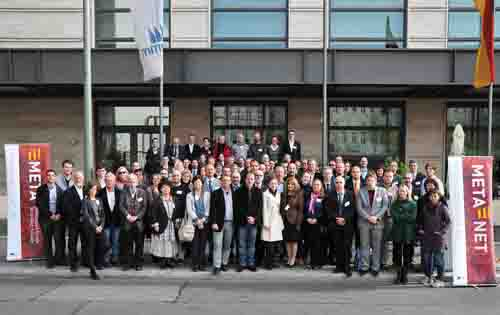
\includegraphics[width=\textwidth]{../_media/meta-net_team.jpg}
  \caption{Alrededor de 100 expertos en tecnología lingüística -representantes de los países y las lenguas incluídos en META-NET- discutieron y finalizaron los principales resultados y mensajes de la Serie de Libros Blancos de META-NET en una reunión en Berlín, Alemania, los días 21 y 22 de octubre de 2011. --- \textcolor{grey1}{About 100 language technology experts -- representatives of the countries and languages represented in META-NET -- discussed and finalised the key results and messages of the White Paper Series at a META-NET meeting in Berlin, Germany, on October 21/22, 2011.}}
  \medskip
  \colorrule{grey3}{\textwidth}{1.5pt}
\end{figure*}

\cleardoublepage

\phantomsection\bsection[La serie de Libros Blancos de META-NET -- The META-NET White Paper Series]{La serie de Libros \mbox{Blancos de META-NET} --- The META-NET\ \ \ \ \ \ \ White Paper Series}
\label{whitepaperseries}

\selectlanguage{english}

\vspace*{-5mm}
\centering
  \setlength{\tabcolsep}{2.2em}
  \begin{tabularx}{\textwidth}{lllll} \toprule\addlinespace
  &Alemán & German & Deutsch& \\
  &Búlgaro & Bulgarian & български& \\
  &Catalán & Catalan & català& \\
  &Checo & Czech & čeština& \\
  &Croata & Croatian & hrvatski& \\
  &Danés & Danish & dansk& \\
  &Eslovaco & Slovak & slovenčina& \\
  &Esloveno & Slovene & slovenščina& \\
  &Español & Spanish & español& \\
  &Estonia & Estonian & eesti& \\
  &Finlandés & Finnish & suomi& \\
  &Francés & French & français& \\
  &Gallego & Galician & galego& \\
  &Griego & Greek & ελληνικά& \\
  &Holandés & Dutch & Nederlands& \\
  &Húngaro & Hungarian & magyar& \\
  &Inglés & English & English& \\
  &Irlandés & Irish & Gaeilge& \\
  &Islandés & Icelandic & íslenska& \\
  &Italiano & Italian & italiano& \\
  &Letón & Latvian & latviešu valoda& \\
  &Lituano & Lithuanian & lietuvių kalba& \\
  &Maltés & Maltese & Malti& \\
  &Noruego Bokmål & Norwegian Bokmål & bokmål& \\
  &Noruego Nynorsk & Norwegian Nynorsk & nynorsk& \\
  &Polaco & Polish & polski& \\
  &Portugués & Portuguese & português& \\
  &Rumano & Romanian & română& \\
  &Serbio & Serbian & српски& \\
  &Sueco & Swedish & svenska& \\
  &Vasco & Basque & euskara& \\ \addlinespace \bottomrule
\end{tabularx}
